\section{Introduction}
The ability of robots to acquire, refine, and adapt their body models is crucial for enhancing their locomotion, manipulation, and interaction capabilities. Despite its significance, existing learning frameworks in robotics often neglect the robot's physical structure. Cognitive robotics underscores the importance of the body schema. However, some approaches interpret a robot's body schema as learning kinematic structural properties, while others focus on sensorimotor associations between proprioceptive, tactile, and visual modalities. Constructing a robot body schema is inherently linked to model-based robotics, offering methods for identifying physical attributes grounded in known kinematic structures.

Nevertheless, challenges persist, particularly for floating-base robots, and existing methods need more integration into incremental learning frameworks. This chapter delves into concepts and methods from different disciplines relevant to defining the robot body schema in this work. Additionally, the chapter outlines the connections between these different methods, establishing their importance as a fundamental tool for building the robotic body schema.

This chapter will introduce notions about the various definitions of the body and its physical attributes, encompassing the physical self and concepts like embodiment, body morphology, and the body schema. With these concepts established, the chapter will survey the fundamental bodily features referred to by these definitions. Shifting the discussion to the realm of robotics, these features will be contrasted against those resulting from conventional calibration and identification methods in model-based robotics. Complementary methods supporting the construction of a robot body schema will be presented to complete the picture.

% Self-modeling in robotics is of great importance as it enables robots to anticipate the outcomes of various actions without physically performing them. This capability allows robots to plan and control their actions more effectively, detect and compensate for damage or wear-and-tear, and make better decisions. By creating internal computational models of their physical bodies, robots can become more self-reliant and function better in the world. This self-awareness, achieved through self-modeling, is a fundamental step towards enhancing the autonomy and performance of robotic systems. The ability to simulate their physical selves enables robots to be more adaptive, efficient, and capable of handling real-world challenges.

%As an anchoring point the concept of physical self will be briefly introduced and the relevant features that are pertinent for the discussion will be highlighted. 
% ===========================================================================================
%                                           |                                               |
% -------------------------------------- SECTION -------------------------------------------|
%                                           |                                               |
% ===========================================================================================
%\part{General body concepts}
\section{Different views on the body and its features}

% SUBSECTION ================================================================================
\subsection{The physical self}
%The concept of the physical self is rooted in human psychology and consciousness \cite{Tsakiris2016multisensorybasisself,Overgaard2023selfitsbody}. It generally refers to an individual's perception and evaluation of the physical body, encompassing appearance, abilities, and overall physicality. It involves the subjective experience of one's body and its relation to the environment, supported by sensory modalities like proprioception, touch, and interoception (sense of internal bodily sensations). This concept is explored in psychology, cognitive science, and related fields to understand how individuals perceive and interact with their bodies.
%
%In the context of robotics, although robots lack subjective experiences, self-awareness, and consciousness, the physical self remains a critical concept. Robots must perceive their bodies and positions in space to operate effectively, particularly in unstructured or dynamic environments. Aspects related to the physical self, such as body morphology, embodiment, and the body schema, are crucial considerations in robotics, see Fig.~\ref{fig:overlapping_concepts}. Body morphology, the physical structure of a robot, significantly influences its design based on intended tasks. For example, a robot designed for exploration might feature legs or wheels, while a robot for assembly line tasks may have a robotic arm \cite{Miller2018EmbodimentSituatednessMorphology}. Embodiment in robotics emphasizes how a robot's physical form and sensory-motor capabilities influence its interaction with the environment, shaping its perception and actions within its surroundings \cite{Wainer2006rolephysicalembodiment}. The concept of the physical self in robotics aligns closely with the body schema, representing an awareness of the robot's body, including the location, orientation, and relative motion of its parts.
%
%In robotics, achieving a sense of the physical self is vital, especially for tasks in dynamic environments. Sensors provide information about the robot's orientation, speed, and acceleration, while actuators enable the robot's body to move, allowing it to learn about its physical capabilities through observed effects on the environment. This information contributes to the creation of a model of the robot's body within its internal representation of the world.
The concept of the physical self is rooted in human psychology and consciousness \cite{Tsakiris2016multisensorybasisself,Overgaard2023selfitsbody}. It typically refers to an individual's perception and evaluation of their own physical body, encompassing appearance, abilities, and overall physicality. It involves the subjective experience through diverse sensory modalities (like proprioception and touch) of the body and its relation to the environment. Aspects related to the physical self, such as body morphology, embodiment, and the body schema, are intertwined concepts, see Fig.~\ref{fig:overlapping_concepts}.

In the context of robotics, although robots lack subjective experiences, self-awareness, and consciousness, the physical self remains a critical concept. Robots must perceive their bodies in space to operate effectively in diverse environments. The physical structure of a robot, its body morphology, significantly influences its design based on intended tasks. For example, a robot designed for exploration might feature legs or wheels, while a robot for assembly line tasks may have a robotic arm \cite{Miller2018EmbodimentSituatednessMorphology}. Embodiment in robotics emphasizes how a robot's physical form and sensory-motor capabilities influence its interaction with the environment, shaping its perception and actions within its surroundings \cite{Wainer2006rolephysicalembodiment}. The notion of the physical self in robotics corresponds extensively with the body schema, representing an awareness of the robot's body, including the location, orientation, and relative motion of its parts.

In robotics, achieving a sense of the physical self is vital, especially for tasks in dynamic environments. The sensor suite of a robot provides feedback on the position, orientation, velocity, and acceleration of its body parts. The actuation mechanisms drive the complex motions of the structure, giving the robot the opportunity to acquire knowledge about its physical capabilities through the perceived consequences of its actions on the environment. This information contributes to the creation of a model of the robot's body within its internal representation of the world.
% ---
\begin{figure}
	\begin{center}
		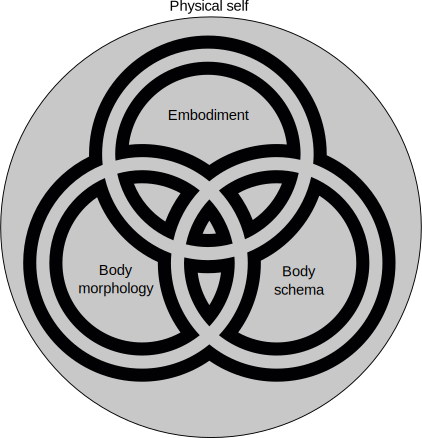
\includegraphics[width=0.5\textwidth]{overlapping_concepts}
		\caption{\textbf{Overlapping concepts.} Embodiment, body morphology, and body schema are three intersection concepts all involved in the definition of the physical self.}
		\label{fig:overlapping_concepts}
	\end{center}
\end{figure}
% ---

% SUBSECTION ================================================================================
\subsection{The body morphology}
The robot body morphology encompasses its physical structure, including the configuration of joints, limbs, sensors, and actuators \cite{Pfeifer2007SelfOrganizationEmbodiment}, playing a pivotal role in determining its capabilities and performance. The joints, serving as points of articulation, allow varied motion, with types like revolute, prismatic, and universal joints offering different degrees of flexibility. Limbs, the appendages extending from the body, consist of links and joints, defining the robot's range of motion and dexterity. Sensors provide information about the environment and internal state, influencing perception and decision-making. Actuators converting energy into mechanical motion and drive joint and limb movement, determining strength and endurance.

Design considerations for robot morphology involve stability, ensuring the robot withstands external forces and maintains balance. Dexterity is crucial for precise movements, achieved through joint, limb, and gripper design. Efficiency minimizes energy consumption for optimal performance, which is vital for autonomous or remote operation. Adaptability allows the robot to meet diverse task requirements or environmental conditions through modular designs or reconfigurable structures. Safety considerations prioritize minimizing risks to the robot and humans around it, incorporating protective tactile elements and elastic joints. Overall, a well-designed robot morphology integrates these key aspects and considerations to enhance its functionality and applicability.

The body morphology of a robot significantly influences its functionality and adaptability. Research in the field of robotics has emphasized the importance of the robot's body in achieving stable locomotion, efficient control, and adaptation to environmental challenges. For instance, the design and control of soft robots have focused on exploiting dynamics and morphology, such as the shape and length of the body and feet, to achieve stable walking \cite{Pfeifer2007SelfOrganizationEmbodiment}. Additionally, studies have shown that morphological variations can be a powerful technique for achieving resilient robots \cite{Pagliuca2020dynamicbodybrain}. Furthermore, it has been hypothesized that the morphological complexity of a robot should scale in relation to the complexity of its task environment \cite{Auerbach2012RelationshipEnvironmentalMechanical}.

In summary, the body morphology of a robot plays a crucial role in its locomotion, adaptability, and task-specific functionality. The research in this field underscores the importance of considering the dynamic interaction between a robot's body and its environment and the potential for co-optimizing morphology and control to enhance the robot's overall performance.

% SUBSECTION ================================================================================
\subsection{The body schema}

\subsubsection{General intuition}
The human body relies on a sophisticated neural representation known as the \textit{body schema} to navigate and interact with the surrounding environment, playing a foundational role in shaping the human experience of the physical self and the external world. This dynamic internal map within the brain encodes a multitude of attributes, ensuring the ability to perceive, move, and coordinate the body effectively.

The concept of the body schema has been defined in various ways in the scientific literature. One common definition is that it consists of sensorimotor representations guiding actions \cite{Maravita2003MultisensoryIntegrationBody}. Alternatively, it is seen as an internal representations of the body's current posture and spatial extension \cite{Vignemont2010Bodyschemabody}. Fundamental to the body schema is the representation of the size and shape of different body parts, allowing for precise and coordinated movements. The brain's ability to accurately map the dimensions of the body contributes to the fluidity of human motion. Additionally, the body schema has been described as a means of obtaining information regarding body position in space from tactile, proprioceptive, visual, and other sensory modalities \cite{Medina2010mapsformspace}. These definitions illustrate the multifaceted nature of the body schema, encompassing sensorimotor guidance, spatial representation, and the integration of multisensory information.

The body schema, a complex and dynamic representation, plays a fundamental role in facilitating our effective interaction with the world. This intricate construct incorporates various properties crucial for our sensory and motor experiences. Spatial properties, encompassing the position, posture, overall shape, and size of individual body parts, as well as the body's relationship to gravity and the environment, form the foundation of the body schema. Kinesthetic properties involve the sensations of movement, touch, generated muscle force, and the resistance encountered during interactions. Vestibular properties contribute to our sense of balance, orientation in space, and awareness of the body's movement through space. Somatosensory properties, including the perception of temperature, pain, and pressure, as well as awareness of the body's surface and internal organs, further enrich the body schema. \redtext{Additionally, the representation of mass, inertia, muscle forces, object properties, environmental properties, body ownership, and body boundaries collectively shape this intricate representation REF}. Adaptability and plasticity enable adjustments through experience and learning. By integrating these diverse elements, the body schema enables humans to navigate their surroundings, interact with objects, and maintain a coherent sense of self in dynamic environments \cite{Vignemont20213C1Whatisbody,Morasso2015Revisitingbodyschema,Asada2018168Proprioceptionbodyschema}.


\subsubsection{The robot body schema}
Generally, the notion of body schema comprises sensorimotor representations of the body used to guide movement and action \cite{Asada2018168Proprioceptionbodyschema}. For robotics this is, however, a far too general definition and incites the question: \textit{what concretely is the body schema in robotics?} From the various takes on this topic, efforts to consolidate an answer to this baffling question were provided in the comprehensive work by Hoffmann et al. \cite{Hoffmann2010Bodyschemarobotics}. Relevant to this dissertation is the discussion that the authors provide on explicit, articulated, and implicit models of the body schema. The first two categories correspond to models where there is a direct correspondence between the body parts of
the robot and their representation in the model, given measured variables that can be associated to properties of the physical body. The main difference being that articulated models \cite{Grush2004emulationtheoryrepresentation} emphasize that the signals ought to come from embodied sensors. This latter property has been referred as subjective or situated body schema \cite{Hersch2008Onlinelearningbody}. The third category, implicit body schema, is more inline with traditional model learning methods in robotics and is aimed at constructing sensorimotor mappings.

%As accentuated by the rich literature in model-based robotics, models of robots are required to achieve fine control and perform complex tasks. These models should include as much information as possible, explicit or implicit, of their body morphology (its embodiment). Most of the efforts associated with learning the body schema agree on the argument that an embodied robotic agent must autonomously learn and refine its body schema relying mainly proprioceptive information \cite{Morasso2015Revisitingbodyschema, Hoffmann2010Bodyschemarobotics}. Yet, in spite of the many bodily features encoded in the body schema, the majority of research focus on calibration of a known kinematic structure \redtext{REF} and only a few works address the discovery of the body topology \redtext{REF}. \redtext{It is worth mentioning that there is no solid consensus in the literature about whether the body schema includes the inertial description of the parts composing the body. Yet, given that the body schema is used for planning and executing movements and that the sensation of effort (force and torque) is part of proprioception, it seems reasonable to assume the body schema must incorporates such a representation.} ultimately, the question remains of what constitutes a body schema in robotics. 
%
%To continue the discussion in this work the following conceptual definition of the robot body schema will be used:
%
%\begin{definition}\label{def:robot_body_schema}
%	%	The robot body schema is a representation of its body morphology that is mainly built from proprioceptive information. This representation includes the arrangement, geometry, and inertial properties of its parts and grants the ability to perceive the relative positions of limbs, and plan and execute movements without relying on visual cues. Adaptive and self-acquired, the robot body schema is a fundamental part of forward and inverse models used to plan and predict sensorimotor interactions beyond proprioception.
%	The robot body schema is a representation of its body morphology primarily constructed from proprioceptive information. This representation encompasses the arrangement, geometry, and inertial properties of its parts, providing the capacity to perceive the relative positions of limbs and to plan and execute movements without relying on visual cues. Adaptive and self-acquired, the robot body schema plays a fundamental role in forward and inverse models, aiding in the planning and prediction of sensorimotor interactions beyond proprioception.
%\end{definition}
%% ---

% SUBSECTION ================================================================================
\subsection{Embodiment}
Embodiment, rooted in the notion that intelligence necessitates a body \cite{Pfeifer2006Howbodyshapes}, is a key concept in robotics. In this context, it refers to how a robot's physical form and sensory-motor capabilities shape its interactions within its environment, influencing perception and actions \cite{Duffy2000Intelligentrobotsquestion}. This involves considerations of the robot's physical structure, situatedness, and morphology, extending beyond functionality to impact interactions with the external world \cite{Miller2018EmbodimentSituatednessMorphology}.

At the core of embodiment is the physical form and morphology of a robot, including joints, limbs, sensors, and actuators. Beyond aesthetics, the design of a robot's physical form significantly influences movement, interaction capabilities, and overall functionality \cite{Pfeifer2006MorphologicalComputationConnecting}. Engineers delve into nuances of body morphology to tailor robots for specific tasks, whether exploration or assembly line operations.

Embodying robots goes beyond external structure, emphasizing that artificial agents have physical bodies interacting with the environment through seamless sensorimotor integration \cite{Lara2018EmbodiedCognitiveRobotics}. Sensors act as receptors conveying information, and actuators enable the robot to act upon sensory input, resulting in adaptive behavior \cite{Pfeifer2007SelfOrganizationEmbodiment,Der2014RoleEmbodimentSelf}. This sensorimotor integration distinguishes embodied robotics from abstract computational systems.

Embodiment also involves situatedness, where robots directly interact with their environment, enhancing autonomy and adaptability \cite{Brooks1991NewApproachesRobotics}. Incorporating action and sensory-motor experiences as sources of statistical regularities is crucial for cognitive robots \cite{Pezzulo2013ComputationalGroundedCognition}.

The concept of body schema, closely linked to embodiment, represents an internal model encompassing a robot's body arrangement, geometry, and movements. It serves as a dynamic tool for spatial awareness. Adaptability is a hallmark of embodied robots, stemming from the close coupling of their physical bodies and control systems, enabling dynamic responses to environmental changes.

In essence, embodiment in robotics transcends traditional boundaries, transforming robots into physically present, interactive agents. The intricate dance between physical form, sensorimotor integration, body schema, and adaptability enriches robotics, fostering the development of sophisticated, versatile, and context-aware systems.

% SUBSECTION ================================================================================
\subsection{Summary of the body concepts}
The physical self, embodiment, body schema, and body morphology are interconnected concepts crucial for understanding human self-awareness and interaction with the world. The physical self involves our awareness of our body and its movements, incorporating proprioception and interoception. Embodiment posits that our thoughts and experiences are shaped by our physical bodies, influencing our mental representations of the world. The body schema, a dynamic internal model, reflects our body's structure and spatial position based on sensory feedback. Body morphology, encompassing size and shape, affects movement and interactions. These concepts are interrelated, with the physical self serving as the foundation for embodiment, the body schema manifesting embodiment, body morphology influencing embodiment, and embodiment shaping the physical self. In the realm of robotics, these concepts are pertinent for robots to effectively interact with the world, requiring a sense of their physical selves and an understanding of embodiment to develop grounded behaviors. Table~\ref{tab:body_concepts} condenses the meaning and relationships of these body concepts.
% ---
\begin{table}
\begin{center}
	\begin{tabular}{ |m{0.3\textwidth}|m{0.34\textwidth}|m{0.34\textwidth}| } 
		\hline
		\textbf{Concept} & \textbf{Definition} & \textbf{Relationship} \\ 
		\hline
		Physical self & Our awareness of our own body and its interactions with the environment & Foundation of embodiment \\ 
		\hline
		Embodiment & The idea that our thoughts, feelings, and experiences are shaped by our physical bodies & Dynamic representation of body's physical structure and position in space \\ 
		\hline
		Body schema	 & Our internal model of our body's physical structure and its position in space & Manifestation of embodiment \\ 
		\hline		
		Body morphology & The physical structure of our body, including its size, shape, and proportions & Influences embodiment and the physical self\\
		\hline
	\end{tabular}
\end{center}
\caption{\textbf{Relationships between the body concepts}}
\label{tab:body_concepts}
\end{table}
% ---	



% ===========================================================================================
%                                           |                                               |
% -------------------------------------- SECTION -------------------------------------------|
%                                           |                                               |
% ===========================================================================================
\section{Robot body representation}
In the subsequent discussion, embodiment and robot morphology will be considered as almost equivalent concepts that relate to the actual physical attributes of the robot body. As accentuated by the rich literature in model-based robotics, models of robots that capture these attributes are required to achieve fine control and perform complex tasks. These models should include as much information as possible, explicit or implicit, of their body morphology (or embodiment). Most of the efforts associated with learning the body schema agree on the argument that an embodied robotic agent must autonomously learn and refine its body schema relying mainly proprioceptive information \cite{Morasso2015Revisitingbodyschema, Hoffmann2010Bodyschemarobotics}. Yet, in spite of the many bodily features encoded in the body schema, the majority of research focus on calibration of a known kinematic structure \redtext{REF} and only a few works address the discovery of the body topology \redtext{REF}. \redtext{It is worth mentioning that there is no solid consensus in the literature about whether the body schema includes the inertial description of the parts composing the body. Yet, given that the body schema is used for planning and executing movements and that the sensation of effort (force and torque) is part of proprioception, it seems reasonable to assume the body schema must incorporates such a representation.} ultimately, the question remains of what constitutes a body schema in robotics. 

To continue the discussion in this work the following conceptual definition of the robot body schema will be used:
% ---
\begin{shaded}
	\begin{definition}\label{def:robot_body_schema}
		%	The robot body schema is a representation of its body morphology that is mainly built from proprioceptive information. This representation includes the arrangement, geometry, and inertial properties of its parts and grants the ability to perceive the relative positions of limbs, and plan and execute movements without relying on visual cues. Adaptive and self-acquired, the robot body schema is a fundamental part of forward and inverse models used to plan and predict sensorimotor interactions beyond proprioception.
		The robot body schema is a representation of its body morphology primarily constructed from proprioceptive information. This representation encompasses the arrangement, geometry, and inertial properties of its body parts, providing the capacity to perceive their state of motion and to plan and execute movements independent from visual inputs. Adaptive and self-acquired, the robot body schema plays a fundamental role in forward and inverse models, aiding in the integration, planning and prediction of sensorimotor interactions beyond proprioception.
	\end{definition}
\end{shaded}
% ---

% SUBSECTION ================================================================================
\subsection{Proprioception}
Proprioception, crucial for executing coordinated movements, refers to the sense of the position and movement of the body or its segments \cite{Kenzie2017compositeroboticbased}. The signals emanate from mechanoreceptors (proprioceptors) like muscle spindles or Golgi tendon organs, embedded in joints, muscles, and tendons \cite{Proske2012proprioceptivesensestheir}. These receptors detect distinct features, such as joint position, movement, and effort. Proprioceptive signals are transmitted to the central nervous system, where they are integrated with information from other sensory systems, such as the visual and vestibular systems, to create an overall representation of the body's motion and orientation. This representation is essential for motor coordination and recovery. Proprioception is generally categorized into two submodalities: kinaesthesia, the sense of limb movement, and joint position sense, the sense of limb position \cite{DAntonio2021RoboticAssessmentWrist,Hillier2015AssessingProprioceptionSystematic}.

Proprioceptive signals inform an agent about the position and movement of limbs and trunk, enabling it to maneuver the body around obstacles even in poor visibility conditions. Similarly, proprioception---in combination with the body schema---allows the manipulation of objects outside the field of vision. Traditionally confined to conscious sensations, proprioceptors include receptors for kinesthetic sensations (position, movement, balance), and those related to effort (tension, force, heaviness). The latter being directly in association  with motor commands. Indeed, various proprioceptive sensations can be attributed to a centrally originated sense of effort \cite{Proske2012proprioceptivesensestheir}. Lastly, a fundamental role of proprioception is to ensure the plasticity of the body schema \cite{Cardinali2016Proprioceptionisnecessary}.

% SUBSECTION ================================================================================
\subsection{Robot proprioception}
%\begin{figure}
%	\begin{center}
%		\includegraphics[width=0.99\textwidth]{example-image-a}
%		\caption{\textbf{Examples of proprioceptive sensors.}}
%		\label{fig:example_proprioceptive_sensors}
%	\end{center}
%\end{figure}
Akin to biological agents, robot proprioception refers to a robot's ability to sense and perceive the position, movement, orientation, and effort of its own body parts. Similar to how humans rely on proprioception to be aware of their body's position and movement, robots leverage proprioceptive capabilities to understand their own kinematics and dynamics. This information is crucial for robots to execute precise and coordinated movements, adapt to changes in their environment, and interact effectively. Typically, robotic proprioception is provided by the following sensors\cite{Siegwart2011Introductionautonomousmobile}:
% ---
\begin{itemize}
	\item \textbf{Joint Encoders:} Sensors that measure the angular position of each joint in a robot. They provide feedback on the angular displacement of the joints, allowing the robot to determine its joint angles accurately. Conventionally, numerical differentiation of these signals are used to convey joint velocity.
	
	\item \textbf{Gyroscopes:} They measure the rate body angular velocity of a body. They help in determining the robot's orientation and changes in orientation over time. Gyroscopic sensors contribute to maintaining stability and control in dynamic motions.
	
	\item \textbf{Accelerometers:} Accelerometers measure the linear acceleration of a body in various directions. By integrating acceleration data over time, robots can derive information about velocity and its changes. Accelerometers are vital for tasks requiring dynamic motion analysis.
	
%	\item \textbf{Inertial Measurement Units (IMUs):} IMUs combine data from accelerometers and gyroscopes to provide comprehensive information about a robot's linear acceleration and angular velocity. IMUs are often used for estimating the robot's pose (position and orientation) in three-dimensional space.

	\item \textbf{Force/Torque Sensors:} Force and torque sensors measure the wrench applied to a robot's end-effector or joints. These sensors provide feedback on external forces acting on the robot, enabling it to respond and adapt to interactions with objects or the environment.
	
	\item \textbf{Vibration sensors:} Vibration sensors measure the vibration of a robot's body. They can be used to detect collisions with objects and to maintain stability in uneven terrain.
	
	\item \textbf{Strain Gauges:} Strain gauges are used to measure deformation or strain in robot components, providing information about the stress and load on specific parts. This is useful for monitoring structural integrity and preventing mechanical failures.
	
\end{itemize}
% ---

%Apart from the typical measurements of the robot's joint position $ q $, velocity $ \dot{q}$, and joint torque $ \tau $, the use of inertial measurement units (IMU) to measure the acceleration $ \dot{\bm{v}} $ and angular velocity $\bm{\omega}$ of the robot's bodies has had applications in state \cite{DeLuca2007accelerationbasedstate} and joint velocity and acceleration estimation \cite{Birjandi2019Jointvelocityacceleration, Rotella2016Inertialsensorbased}, the control of mobile robots \cite{Dutta2019StabilityAnalysisHumanoid}, and in safe human-robot interaction\cite{Hamad2023ModularizeConquerGeneralized}.

In addition to the standard measurements of joint position $q$, velocity $\dot{q}$, and joint torque $\tau$, using inertial measurement units (IMU) to measure the acceleration $\dot{\bm{v}}$
and angular velocity $\bm{\omega}$ of the robot bodies has been used in state estimation \cite{DeLuca2007accelerationbasedstate}, kinematic estimation from incomplete sensor readings \cite{Rollinson2013RobustStateEstimation}, joint velocity and acceleration estimation \cite{Birjandi2019Jointvelocityacceleration, Rotella2016Inertialsensorbased}, mobile robot control \cite{Dutta2019StabilityAnalysisHumanoid}, and safe human-robot interaction \cite{Hamad2023ModularizeConquerGeneralized}.

%\redtext{Vestibular properties are associated with the body schema, as evidenced by research indicating that vestibular signals play a role in modifying the body schema. Vestibular stimulation has been shown to influence the body schema, impacting the relative metric properties of body parts and contributing to more abstract cognitive representations of the body. Additionally, there is increasing evidence that vestibular signals and the vestibular cortex are involved in not only oculomotor and postural control, but also in the sense of body, self, and others. While vestibular signals may not serve to scale the internal representation of large parts of the body's metric properties, they do contribute to the body schema and its cognitive representations. Therefore, the vestibular system and its signals are integral to the body schema, impacting various aspects of bodily awareness and cognitive representations of the body.}
%
%Citations:
%[1] https://www.sciencedirect.com/science/article/abs/pii/S0028393212001595
%[2] https://www.sciencedirect.com/science/article/abs/pii/S0028393213001218
%[3] https://open-mind.net/papers/@@zipview?comment=b03b62165a8c49df995cc0ab1e54da66&reply=4476da22bba84972b9c236d737008214&target=e04f7dbea19a4d96a348f678bf07b8bc&type=pdf
%[4] https://www.allpsych.uni-giessen.de/rauisch10/readings/Angelaki&Cullen.AnnuRevNeuro.2008.pdf
%[5] https://www.researchgate.net/publication/224914418_Vestibular_stimulation_modifies_the_body_schema 

%Robot proprioception, enabled by these diverse sensors, allows robots to operate autonomously, adapt to dynamic environments, and execute tasks with precision and efficiency.

% SUBSECTION ================================================================================
\subsection{Body features in the body schema}
%The body schema serves as a link structure that outlines connections among components in the robot arm. This explicit model relies on predefined parameters, with joint angles, typically measured using encoders, tracking the trajectory based on proprioception. In contrast, implicit models are applied in uncalibrated systems, where interaction with the environment estimates desired parameters. This mechanistic approach differs from the biological case, where the inherently flexible link structure adapts to changes in the environment and the self-body. Unlike in robotics, where knowledge is externally provided at a high cost for parameter estimation, biological systems are inherently self-learning, aligning with implicit model principles. Additionally, robotics lacks cross-modal association, whereas the integration of multi-modal sensory information is fundamental in the biological case, emphasizing sophisticated adaptability and sensory integration \cite{Asada2018168Proprioceptionbodyschema}.


%The concept of body schema and its relevance to model learning in robotics is well-supported in the scientific literature. While there are no specific sources directly linking the concept of body schema to model learning in robotics, the following sources provide relevant information about the body schema and its implications:
%\hrule
%\subsubsection{Definition}
%Proprioception refers to the sense of the position and movement of the body or body segments, and it is vital for executing coordinated movements \cite{Kenzie2017compositeroboticbased}. Proprioceptive signals arise from mechanoreceptors (proprioceptors) embedded in the joints, muscles, and tendons, such as muscle spindles or Golgi tendon organs \cite{Proske2012proprioceptivesensestheir}. In general, two submodalities of proprioception are distinguished: kinaesthesia, which is the sense of limb movement, and joint position sense, which is the sense of limb position \cite{DAntonio2021RoboticAssessmentWrist}.
%
%\TODO Paraphrase the following text$\ldots$
%In robotics, the body schema functions as a link structure that delineates the connections among components in the robot arm, incorporating predetermined length and movable range data for each link. This explicit model relies on pre-defined parameters, and joint angles, typically measured using encoders, track the trajectory based on proprioception. In contrast, implicit models find application in uncalibrated systems, where interaction with the environment is employed to estimate desired parameters. This mechanistic approach contrasts sharply with the biological case, where the link structure is inherently flexible, adapting to changes in both the environment and the self-body. Unlike in robotics, where knowledge is externally provided at a high cost for parameter estimation, biological systems are inherently self-learning, aligning with the principles of implicit models. Furthermore, the absence of cross-modal association is a hallmark of robotics, whereas the integration of multi-modal sensory information stands as a fundamental aspect of the biological case, emphasizing the sophisticated adaptability and sensory integration inherent in biological systems \cite{Asada2018168Proprioceptionbodyschema}.
%
%
%The position and movement of limbs and the trunk are informed by sensations arising in proprioceptors, allowing maneuvering around obstacles in the dark and manipulation of objects out of view. Traditionally, the term proprioceptor has been confined to receptors concerned with conscious sensations, encompassing limb position, movement, tension, force, effort, and balance. The importance of robot proprioception is underscored by examining its role in living systems. The distinction between kinesthetic sensations and those related to effort, force, and heaviness is considered, emphasizing that the latter are invariably associated with motor commands. It is concluded that various proprioceptive sensations, including limb position and movement, can be contributed to by a centrally originated sense of effort \cite{Proske2012proprioceptivesensestheir}. Furthermore, studies have regarded proprioception as fundamental to ensure the plasticity of the body schema \cite{Cardinali2016Proprioceptionisnecessary}.


%\subsubsection{The role of proprioception}
%Much of this knowledge about position and movement of the limbs and trunk is provided by sensations arising in proprioceptors. The information they provide allows us to maneuver
%our way around obstacles in the dark and be able to manipulate objects out of view.
%
%Traditionally, however, the term proprioceptor has been restricted to receptors concerned with
%conscious sensations, and these include the senses of limb position and movement, the sense of tension or force, the sense of effort, and the sense of balance.
%
%To motivate the importance of robot proprioception, this section first discusses the role it plays in living systems. This section relies on the material presented in As proprioceptive sensations, the senses of effort, force, and heaviness are distinct in that they are always associated with motor commands, while kinesthetic sensations can arise in a passive limb. It implies that for the senses of force and heaviness the peripheral input is always reafferent in origin. Another issue to consider is the meanings of the terms. What do we mean by a sense of effort as distinct from a sense of tension?
%
%It is concluded that a sense of effort, arising centrally in association with motor commands, is able to contribute to a number of proprioceptive sensations including the sense of limb
%position and the sense of limb movement.

%\subsubsection{A sensor suite for robot proprioception}
%\TODO

%\subsection{Essential body features}
% ---
\begin{figure}
	\begin{center}
		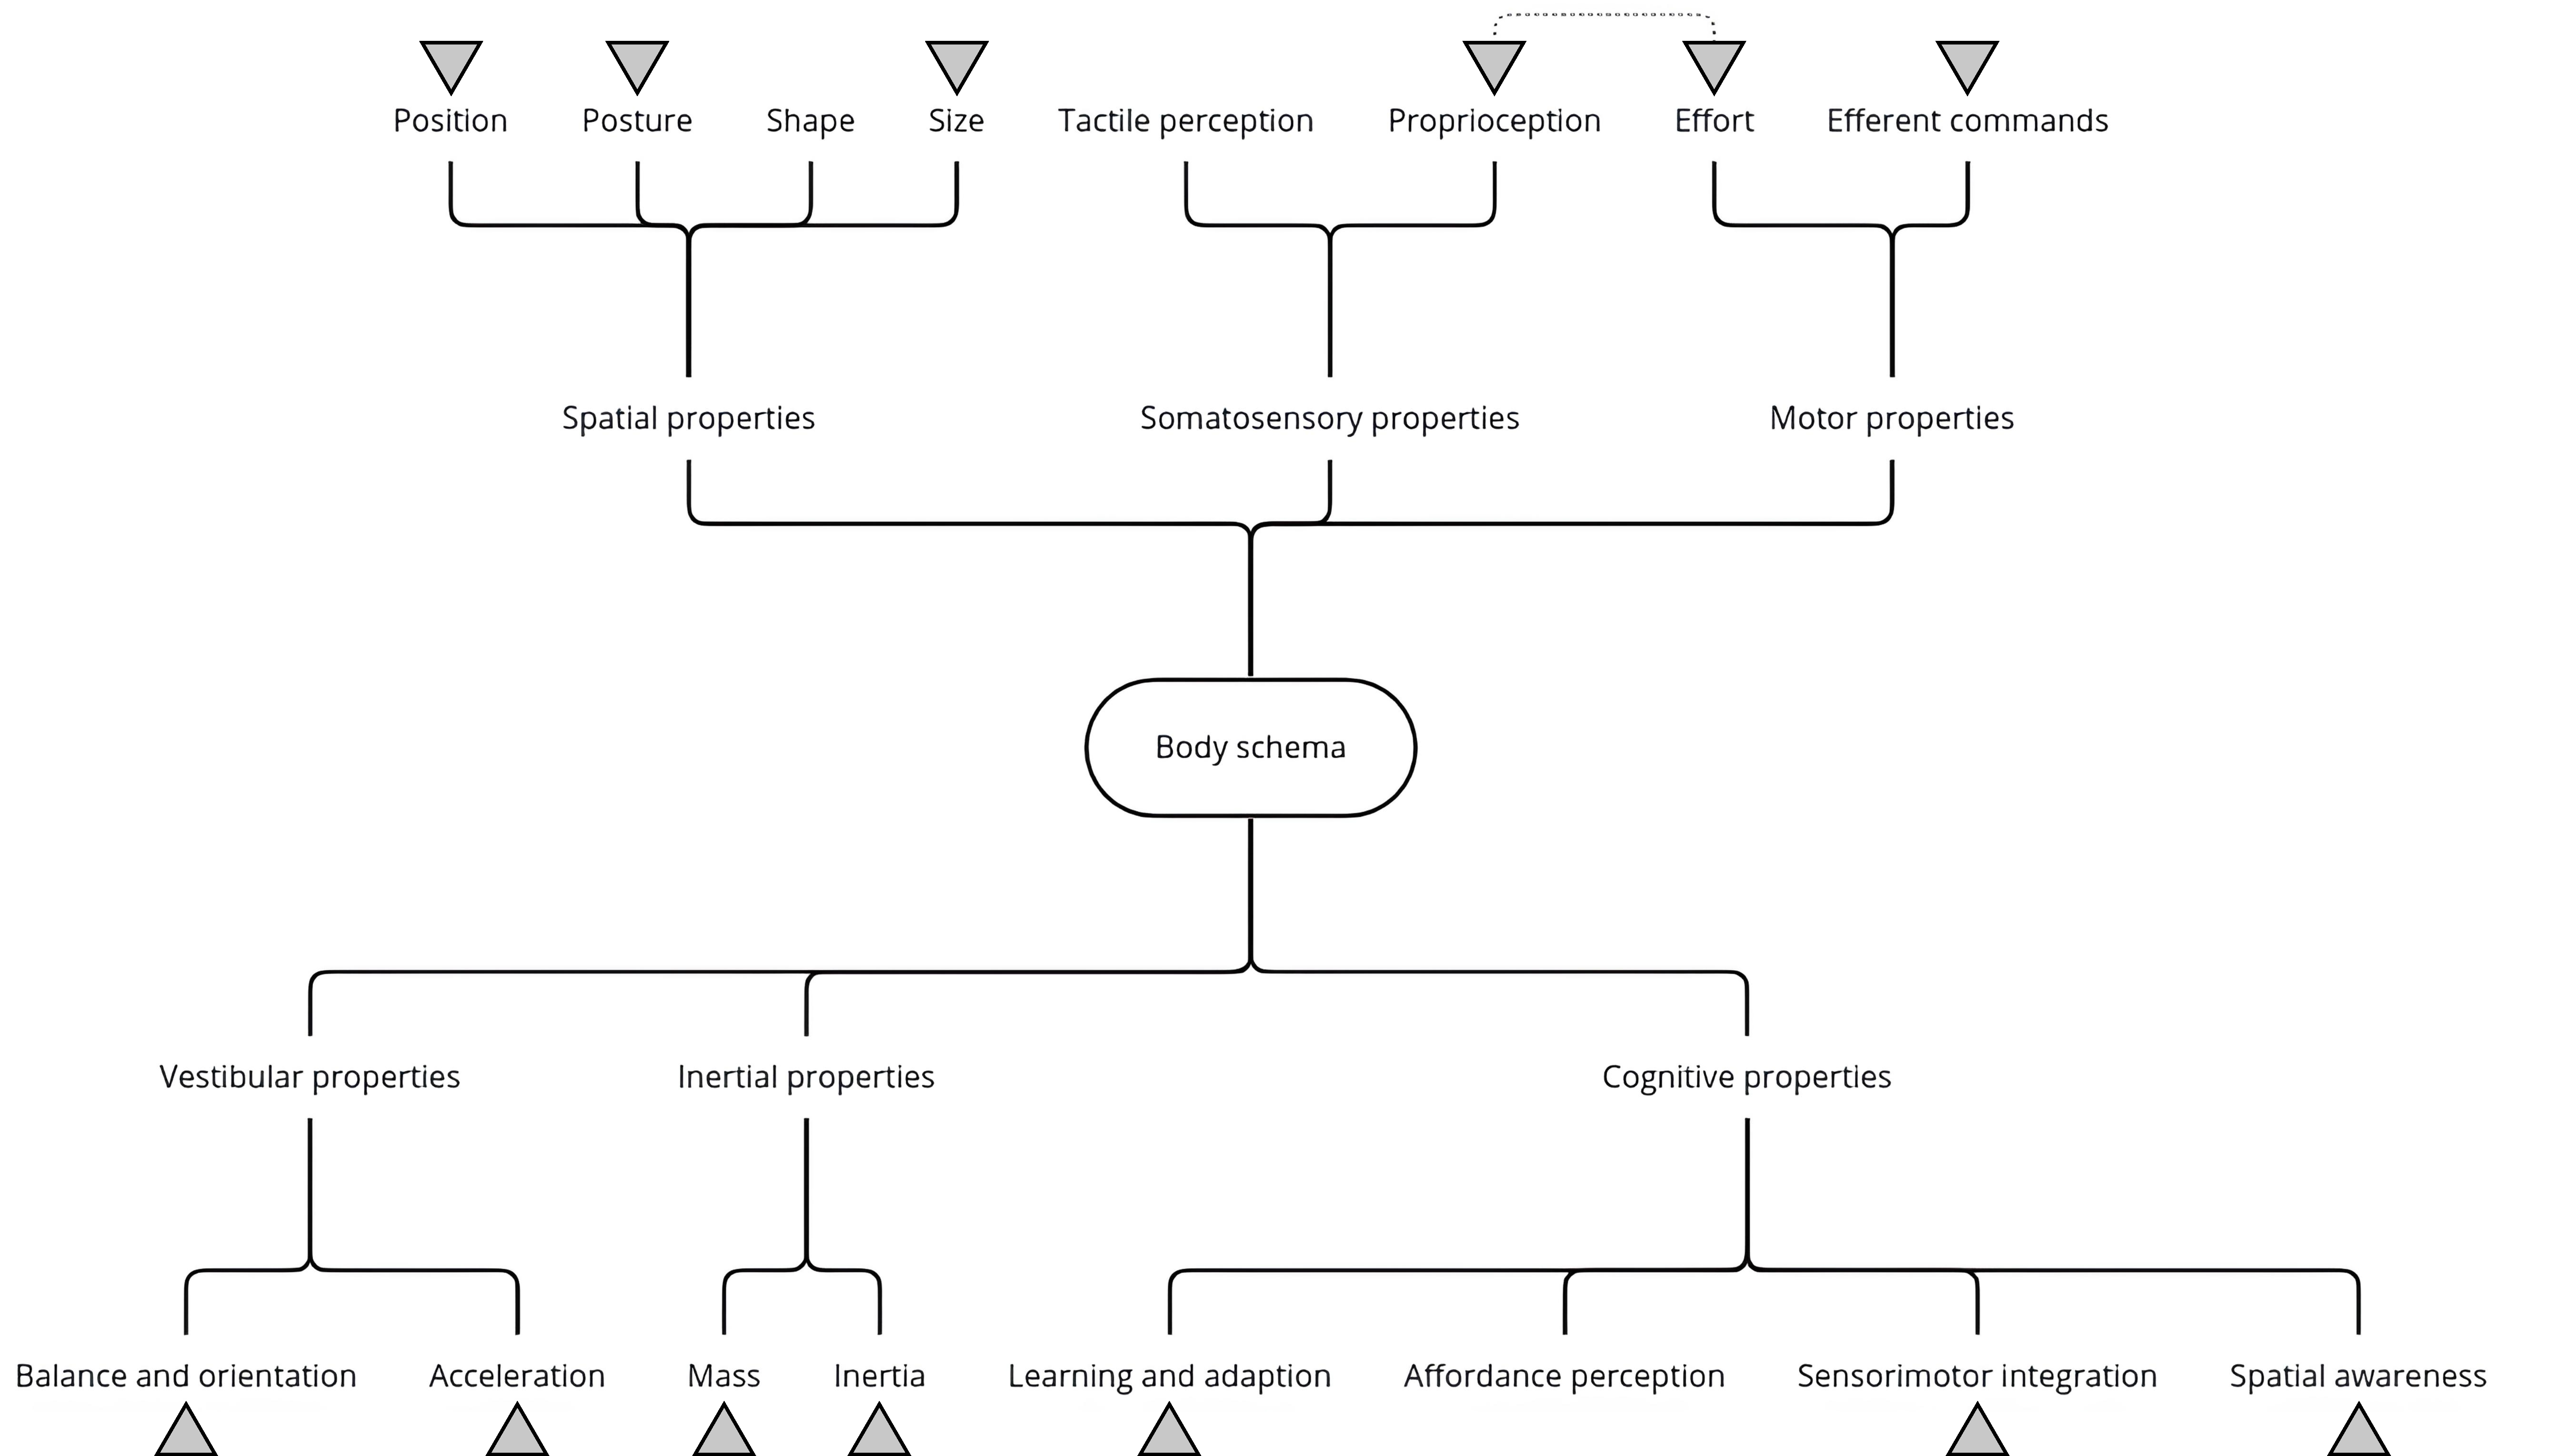
\includegraphics[width=0.99\textwidth]{body_schema_properties.pdf}
		\caption{\textbf{Properties of the body schema.} The body schema subsumes several properties of the body morphology and results in cognitive properties resulting from the robot embodiment.}
		\label{fig:body_schema_properties}
	\end{center}
\end{figure}
% ---

The body schema representation encodes various attributes of the body morphology (see Fig.~\ref{fig:body_schema_properties}). %These attributes include:

\paragraph*{Spatial properties} The brain has a representation of the size and shape of different body parts. This allows for accurate and coordinated movements and interactions. Additionally, the body schema includes information about the spatial orientation and position of body parts in relation to each other. This is essential for coordinating movements and maintaining balance.

\paragraph*{Somatosensory properties} Proprioception is the sense of the relative position of one's own body parts and the effort being employed in movement. Proprioceptive information helps in knowing the positions of limbs without having to visually observe them. The body schema encodes information about the angles and movements of joints, allowing for smooth and coordinated motor control. Sensations related to touch, pressure, temperature, and pain are integrated into the body schema. This information helps in perceiving and responding to stimuli from the external environment.

\paragraph*{Vestibular properties} Vestibular signals play a critical role in maintaining balance, spatial awareness, and facilitating coordinated movements. These signals offer vital information about the body's orientation in space, encompassing both linear and angular motion states. Whether engaged in locomotion, manipulation, or adjusting posture, vestibular signals seamlessly collaborate with proprioception. From everyday activities like walking to more intricate movements such as reaching, these signals intricately shape the body schema.

\paragraph*{Inertial properties} 
The inertial properties within the body schema encompass characteristics associated with the mass distribution and moments of inertia of the body. This knowledge holds crucial significance for both forward and inverse models in motor control. In the process of planning a movement, the inertial properties of the body schema come into play as they are utilized to estimate the forces and torques necessary for moving various body parts. Subsequently, this information is employed to generate motor commands. These properties, working in conjunction with vestibular information, play a pivotal role in maintaining balance.
%The inertial properties of the body schema refer to the characteristics related to the body's mass distribution and moments of inertia. This knowledge is essential for forward and inverse models for motor control. When planning a movement, inertial properties of the the body schema are used to estimate the forces and torques required to move different parts of the body. This information is then used to generate motor commands that accurately control the movements of our muscles. These properties play an important role together with vestibular information in maintaining balance.
%The body schema continuously updates its representation of the body's position, orientation, and mass distribution to maintain balance. 

\paragraph*{Cognitive properties} The body schema enables the representation of body parts' position and orientation in space, facilitating tasks like reaching, grasping, and navigating. It also helps perceive the affordances of objects, indicating how they can be used. Enables meaningful interaction with objects based on their properties. Learning and Adaptation: The body schema's plasticity allows constant updates, incorporating new movements, environmental interactions, and changes in the body for improved motor performance and adaptation. Lastly, the body schema integrates information from various sensory modalities—sight, touch, proprioception, and vestibular input.

\paragraph*{Motor Properties} The body schema is closely tied to motor control and the execution of movement. It helps in generating and executing motor programs for voluntary actions.

% SUBSECTION ================================================================================
\subsection{Learning the body schema}
Model-based robotics is inherently linked to the concept of the body schema, as defined in Def.~\ref{def:robot_body_schema}. It encompasses a theoretical foundation and methods that consider the physical properties of robots and integrate them into their representations. However, these methods often treat body properties as immutable, relying on a single identification or calibration procedure. Some studies have compared the conventional characteristics of model-based robotics, such as being amodal, fixed, explicit, centralized, and modular, with the properties of a biological body schema \cite{Hoffmann2021Bodymodelshumans}. Unlike robotic body models, the body schema is dynamic, capable of modification based on experiences, learning, and changes in the body itself. Additionally, biological systems are inherently self-learning and rely on the integration of multi-modal sensory information \cite{Asada2018168Proprioceptionbodyschema}.

The integration of learning techniques with model-based robotics allows conventional fixed descriptions to adapt. Frameworks that exploit and extend this combination bring traditional model-based body models closer to a body schema, enabling robots to construct, monitor, and adjust their understanding of their bodies by integrating information from multiple sensory modalities. Consequently, this integration aligns more closely with the concept of the robot body schema. This dissertation focuses on a subset of the body schema properties highlighted in Fig.~\ref{fig:body_schema_properties}, marked with triangles in the figure. The subsequent discussion will survey frameworks and methods that have been employed or could be utilized to infer quantities directly connected to the highlighted properties of the robot body schema.

%First, we define the self as a set
%S = {N, A, λ, θ},
%(1)
%whose elements are the number of degrees of freedom (i.e.
%links) N , the adjacency matrix A of the robot defining
%the connectivity of the kinematic tree, the morphological
%description of every link in the robot λ, and the inertial
%parameters of the links θ.
%Figure 1 shows how elements of S are found in three dif-
%ferent inverse dynamics identification/learning frameworks.
%Fig. 1a shows that classical system identification assumes
%a known calibrated kinematic model (i.e., N , A, λ) and
%mostly focuses on learning θ

%\redtext{The body schema outlines connections among components in the robot morphology. Explicit models rely on predefined parameters, typically identified measured using encoders, tracking the trajectory based on proprioception. In contrast, implicit models are applied in uncalibrated systems, where interaction with the environment estimates desired parameters. This mechanistic approach differs from the biological case, where the inherently flexible link structure adapts to changes in the environment and the self-body. Unlike in robotics, where knowledge is externally provided at a high cost for parameter estimation, biological systems are inherently self-learning, aligning with implicit model principles. Additionally, robotics lacks cross-modal association, whereas the integration of multi-modal sensory information is fundamental in the biological case, emphasizing sophisticated adaptability and sensory integration \cite{Asada2018168Proprioceptionbodyschema}.}


%Model-based robotics is naturally connected to the concept of body schema as per Def.~\ref{def:robot_body_schema}, it includes a theoretical groundwork and methods that take into account physical properties of robots and include them in their representations. Yet, the body properties within the scope of these methods are typically considered immutable and are inferred from a single identification or calibration procedure. Some works have contrasted the conventional amodal, fixed, explicit, centralized, and modular representations provided by model-based robotics against the properties of a biological body schema \cite{Hoffmann2021Bodymodelshumans}. Indeed, unlike body models in robotics, the body schema is not fixed but can be modified based on experiences, learning, and changes in the body itself. Moreover, biological systems are inherently self-learning and depend on the integration of multi-modal sensory information \cite{Asada2018168Proprioceptionbodyschema}.
%
%Combining model-based robotics with learning techniques makes conventional fixed descriptions capable of adaptation. Frameworks that leverage and expand this combination make conventional model-based body models closer to a body schema allowing robots to build, monitor, and adapt the understanding of their bodies integrating information from multiple sensory modalities. Therefore, from this combination it is possible to be more in line with the concept of the robot body schema. In this dissertation attention is given to a subset of the body schema properties in Fig.~\ref{fig:body_schema_properties}, identified with triangles in the figure. In the following discussion frameworks and methods that have been used or could be used to infer quantities that have a direct connection with the highlighted properties of the robot body schema will be surveyed.


%\say{The concept of body schema is related to model learning in robotics as it provides a framework for robots to understand and represent their own bodies and the surrounding environment. Research in this area aims to enable robots to improve their capabilities by automatically synthesizing, extending, or adapting a model of their body, similar to how the human body schema allows for adaptive and coordinated movement. This involves integrating information from multiple sensory modalities and controlling complex bodies, which are desirable capabilities for robots. By studying the body representations in biology from a functional or computational perspective, researchers seek to develop robotic systems that can effectively model their own bodies and interact with the environment in a more human-like manner. Therefore, the concept of body schema plays a crucial role in the development of robotic systems that can learn and adapt to their own physical characteristics and the surrounding world.}

% ===========================================================================================
%                                           |                                               |
% -------------------------------------- SECTION -------------------------------------------|
%                                           |                                               |
% ===========================================================================================
\section{Representing properties of the robot body schema}

% SUBSECTION ================================================================================
\subsection{Kinematics: Body size, position, and posture}
The focus in this work is on serial kinematic chains with either fixed or floating bases and revolute joints. This sections revisits the kinematic modeling essentials of such structures.

A serial kinematic chain is a sequence of rigid bodies called links connected by joints. In a serial kinematic chain the output of one joint becomes the input for the next and there are no loops. Robots, such as manipulators, legged robots, and humanoids, are instances of serial kinematic chains. The motion of the robot is achieved by the controlled rotation or translation of each joint.  A robot is said to be of fixed base if the first link in the chain (base link) is rigidly connected to the world. The best example being robot manipulators. On the contrary, in floating base robots, the base and all other links can freely rotate and translate in space. Humanoid robots are a good example of this type.

Robot joints can be classified into various types. One degree of freedom (DOF) joints include revolute joins (rotational motion about the joint axis), prismatic joints (translational motion along the direction of the joint axis), and  helical joints (simultaneous rotation and translation about a screw axis) \cite{Lynch2017Modernrobotics}. Joints can also have multiple degrees of freedom allowing independent translations and rotations about multiple axes. The configuration and number of joints in the chain determine the robot's total DOF. Typically a joint variable $q$ is used to express the translational or angular displacement between the links connected by a one-DOF joint \cite{Xie2003FundamentalsRoboticsLinking}. For a robot with $n$ joints, the configuration is described by the vector $\bm{q} = [q_1,\ldots,q_i,\ldots,q_n]^\intercal$.

Joint axes are modeled as lines in space, represented as a vector, that indicate the direction about which a joint rotates or translates. In general, the range of mobility $\left[a,b\right] $ of a joint is mechanically constrained by upper $a$ and lower $b$ limits. The Cartesian product of all joint ranges is the configuration space of the robot.
%% ---
%\begin{figure}
%	\begin{center}
%		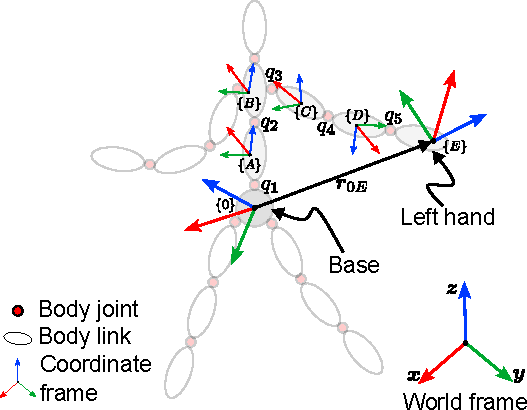
\includegraphics[width=0.5\textwidth]{example_serial_kinematic_chain.pdf}
%		\caption{\textbf{An example of a serial kinematic chain.} A humanoid is a serial kinematic chain with a floating base. Two coordinate frames are shown, one at the base and one at the left hand link.}
%		\label{fig:example_serial_kinematic_chain}
%	\end{center}
%\end{figure}
%% ---

% ---
\begin{figure*}[!t]
	\centering	
	\hspace*{\fill}
	\begin{subfigure}[t]{0.40\textwidth}
		\subcaption{}
		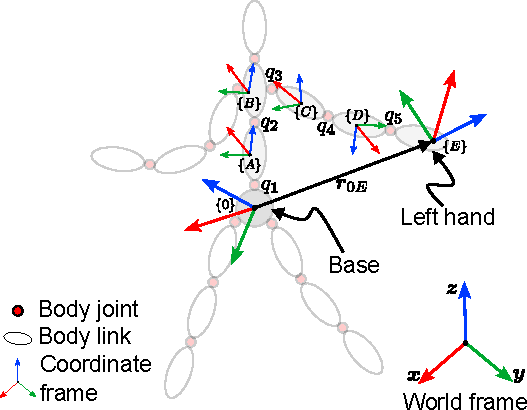
\includegraphics[width=\textwidth]{example_serial_kinematic_chain.pdf}
		\label{fig:example_serial_kinematic_chain}
	\end{subfigure}	
	\hfill
	\begin{subfigure}[t]{0.40\textwidth}
		\subcaption{}
		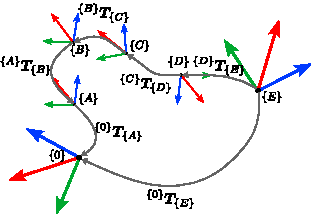
\includegraphics[width=\textwidth]{frame_transformation_sequence.pdf}
		\label{fig:transformation_sequence}
	\end{subfigure}	
	\hspace*{\fill}
	\caption{\label{fig:serial_kinematic_chain} \textbf{A serial kinematic chain and its transformations.} (\subref{fig:example_serial_kinematic_chain})  A humanoid is a serial kinematic chain with a floating base. Two coordinate frames are shown, one at the base and one at the left hand link. (\subref{fig:transformation_sequence}) The sequence of coordinate transformations from frame $\cframe{0}$ to $\cframe{E}$.}
\end{figure*}
% ---

The pose of a rigid body in the kinematic chain represents the position and orientation of a coordinate frame rigidly attached to it with respect to a reference frame \cite{Siciliano2008RoboticsModellingPlanning}. A minimum of six parameters is needed to completely instantiate pose of a rigid body in Euclidean space \cite{Lynch2017Modernrobotics}. The pose of a given body is dependent on all the joint variables from the base to the current joint as well as on the geometry of the links. Considering the simplified humanoid robot shown in Fig.~\ref{fig:example_serial_kinematic_chain} as an example, the link corresponding to the left hand has the frame $\cframe{E}$ rigidly attached to it. Its pose can be expressed relative to the coordinate frame $\left\lbrace 0 \right\rbrace$ located at the humanoid's base link via the homogeneous transformation matrix $^{\{0\}}\bm{T}_{\{E\}}  \in \mathbb{R}^{4\times 4}$ defined as
% ---
\begin{equation}
	^{\{0\}}\bm{T}_{\{E\}} = \begin{bmatrix}
		^{\{0\}}\bm{R}_{\{E\}}(\bm{q}) & ^{\{0\}}\bm{r}_{0E}(\bm{q}) \\
		\bm{0}_{1\times3} & 1
	\end{bmatrix}.
\end{equation}
% ---
The vector $^{\{0\}}\bm{r}_{0E}(\bm{q}) \in \mathbb{R}^3$ denotes the location of the origin of the coordinate frame $\cframe{E}$ relative to and expressed in frame $\cframe{0}$. Similarly, the rotation matrix $^{\{0\}}\bm{R}_{\{E\}}(\bm{q})  \in \mathbb{R}^{3\times 3}$ expresses the orientation of frame $\cframe{E}$ in frame $\cframe{0}$. Both terms are function of the robot configuration vector $\bm{q}$.

A rotation matrix is orthogonal, that is $ \bm{R}^{-1} = \bm{R}^\intercal$, and has unit determinant. Any rotation matrix belongs to the set of all rotation matrices, which is a group known as the rotation group or the special orthogonal group SO(3) \cite{Lynch2017Modernrobotics}. A composition of rotations is achieved by the matrix product of two or more rotation matrices. Similarly, the set of all transformation matrices defines the special Euclidean group SE(3), which represents the group of rigid body motions in 3D space. Just like rotation matrices, all the elements of SE(3) are orthogonal and have determinant equal to 1. Referring back to Fig.~\ref{fig:example_serial_kinematic_chain}, the composition of transformation matrices from the left hand of the humanoid to its base yields the following expression
\begin{equation}
	^\cframe{0}\bm{T}_\cframe{E} = 
	^\cframe{0}\bm{T}_\cframe{A}(q_1)~
	^\cframe{A}\bm{T}_\cframe{B}(q_2)~
	^\cframe{B}\bm{T}_\cframe{C}(q_3)~
	^\cframe{C}\bm{T}_\cframe{D}(q_4)~
	^\cframe{D}\bm{T}_\cframe{E}(q_5),
\end{equation}
a graphical depiction of this sequence of transformations is shown in Fig.~\ref{fig:transformation_sequence}.

In general, the kinematic structure of a robot consists in describing the location and orientation of the frames attached to the composing links. Thus, as homogeneous transformation matrix is associated to each of the $n+1$ rigid bodies in the kinematic chain.

\subsubsection{Representation of transformation matrices}
% ---
\begin{figure}
	\begin{center}
		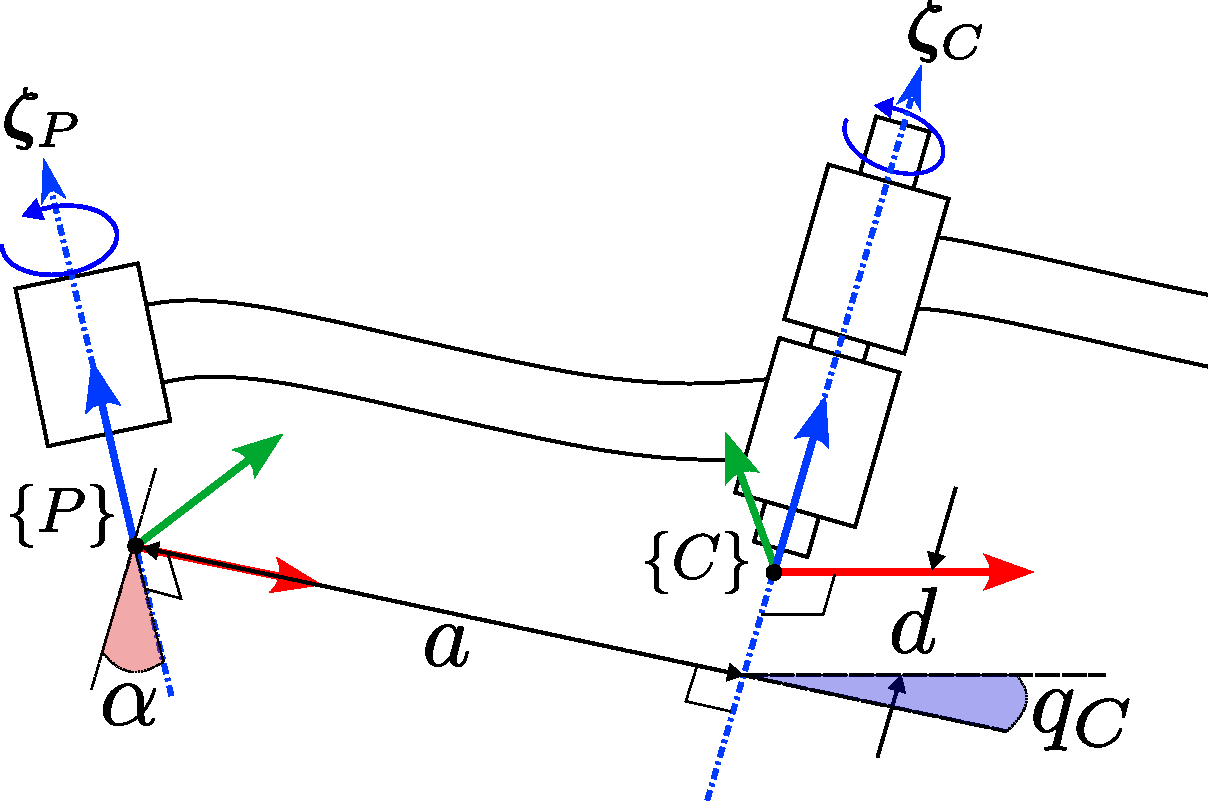
\includegraphics[width=0.5\textwidth]{mdh_frame_convention.pdf}
		\caption{\textbf{MDH frame convention.} The location and orientation of the joint frames in the MDH convention depends on three fixed parameters $(a,\alpha,d)$ and the joint angle $q_C$.}
		\label{fig:mdh_frame_convention}
	\end{center}
\end{figure}
% ---
\paragraph*{Modified Denavit-Hartenberg representation} The modified Denavit-Hartenberg (MDH) convention uses four unique parameters per link to describe the kinematics of robots. With reference to Fig.~\ref{fig:mdh_frame_convention}, the MDH parameters represent the
link length $a$ (the offset distance between the joint axes $\bm{\zeta}_P$ and $\bm{\zeta}_C$), the link twist $\alpha$, the link offset $d$, and the joint angle $q_C$. The set of MDH parameters $\left(a,\alpha,d,q_C\right)$ describe the location and orientation of the joint frames in a robot \cite{Craig1989Introductionroboticsmechanics}. The MDH parameters of a joint are used to define the parameter vector  $\bm{\lambda}^{DH} = \left[\lambda_1,\lambda_2,\lambda_3,\lambda_4\right]^\intercal$ and build with it the following transformation matrix:
% ---
\begin{equation}
 ^\cframe{P}\bm{T}_\cframe{C} =
 \begin{bmatrix}
   	\text{cos}(q_C)         &     -\text{sin}(q_C)    &      0    &      \lambda_1\\      
   	\text{sin}(q_C)\lambda_3& \text{cos}(q_C)\lambda_3& -\lambda_2& -\lambda_2\lambda_4\\
   	\text{sin}(q_C)\lambda_2& \text{cos}(q_C)\lambda_2&  \lambda_3&  \lambda_3\lambda_4\\
   	0                       &         0               &      0    &           1          
 \end{bmatrix},
\end{equation} 
% ---
with $\lambda_1 = a$, $\lambda_2 = \text{sin}(\alpha)$, $\lambda_3 = \text{cos}(\alpha)$, and $\lambda_1 = d$. 

\paragraph*{Euler angles representation} A vector $\bm{\lambda}^{EA} = \left[\lambda_1,\lambda_2,\lambda_3,\lambda_4,\lambda_5,\lambda_6\right]^\intercal$ is used to define a homogeneous transformation matrix based on a rotation matrix 
% ---
\begin{equation}
	      ^\cframe{C}\bm{R}_\cframe{P} = (\text{Rot}_z(\lambda_1)\text{Rot}_x(\lambda_2)\text{Rot}_z(\lambda_3)\text{Rot}_z(q_C))^\intercal
\end{equation}
% ---
depending on the Euler angles \cite{Siciliano2008RoboticsModellingPlanning} $\left(\lambda_1,\lambda_2,\lambda_3\right)$ and the translation vector $ ^\cframe{P}\bm{r}_\cframe{C} = \left[\lambda_4,\lambda_5,\lambda_6\right]^\intercal $. The expression $\text{Rot}_i(j)$ defines a pure rotation of $j$ radians around the axis $i$. 

\paragraph*{Axis-angle representation} A vector of parameters
% ---
\begin{equation}\label{eq:kinematic_parameters}
	\bm{\lambda}^{AA} = \begin{bmatrix}
		^\cframe{P}\bm{\xi}_{C}^\intercal & \phi & ^\cframe{C}\bm{\zeta}_{C}^\intercal & ^\cframe{P}\bm{r}^\intercal_C 
	\end{bmatrix}^\intercal \in \mathbb{R}^{10}
\end{equation}
% ---
is used to define the rotation matrix $^\cframe{P}\bm{R}^T_\cframe{C}$ in axis-angle form \cite{Lynch2017Modernrobotics} as
% ---
\begin{equation}\label{eq:rotation_matrix_axis_angle}
	^\cframe{P}\bm{R}_\cframe{C}\left(q_{C};\bm{\gamma}\right) = \left(\exp^{\left[{^{\left\lbrace P\right\rbrace}}\bm{\xi}_{C}\right]\phi}\right) \left(\exp^{\left[{^{\left\lbrace C\right\rbrace}}\bm{\zeta}_{C}\right] q_C}	\right).
\end{equation}
%---
%with $\bm{\gamma}$ defined as
%% ---
%\begin{equation}
%	\bm{\gamma}=\begin{bmatrix}
%		{^\cframe{P}}\bm{\xi}_{C}^\intercal & \phi & ^{\cframe{C}}\bm{\zeta}_{C}^\intercal
%	\end{bmatrix}^\intercal.
%\end{equation}
% ---
The terms $ \bm{\xi} \in \mathbb{R}^3$ and $ \bm{\zeta} \in \mathbb{R}^3$ being unitary rotation axes and  $ \left[~\cdot~\right] $ denoting a vector $\bm{u} = \left[u_x,u_y,u_z\right]^\intercal$ expressed as a skew-symmetric matrix; i.e.,
% ---
\begin{equation}
	[\bm{u}] = \begin{bmatrix}
		0                & -u_z             & u_y \\
		u_z              & 0                     & -u_x \\
		-u_y             & u_x              & 0
	\end{bmatrix}.
\end{equation}
% ---
The vector $ \bm{\zeta}$ expresses the rotation axis of the joint that connects two bodies, expressed in the coordinate system $\cframe{C}$ of the child body. The angle $\phi$ defines the constant rotation about the axis $\bm{\xi}$ defined by the geometry of the links alone when the joint angle $q_C$ is zero.
% ---
\begin{figure}[t!]
	\begin{center}
		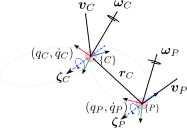
\includegraphics[width=0.5\textwidth]{body_twist_illustration}
		\caption{\textbf{Body twist.} A twist is composed of the linear and angular velocities at a point on a rigid body.}
		\label{fig:body_twist_illustration}
	\end{center}
\end{figure}
% ---


%Revolute joins allow rotational motion about the joint axis, prismatic joints allows translational motion along the direction of the joint axis, and  helical joints allow simultaneous rotation and translation about a screw axis \cite{Lynch2017Modernrobotics}. All these joints have one degree of freedom. Joints can also have multiple degrees of freedom allowing independent translations and rotations about multiple axes.




%For floating and mobile bases, the movement of the robot takes place not only via joint movement but also of the overall translation and rotation of the mechanism in space. As a result the number of degrees of freedom are increased. To represent this in a more straightforward manner, we treat floating base robots as fixed-base robots by means of attaching a virtual linkage that expresses the mobility of the root link.

%It may be improper to think of a "base link" because there is no link attached to the environment, but it is customary to speak of a root link from which calculations begin. For a 2D floating base, the  (𝑥,𝑦)
%translation and rotation  𝜃
%of the robot's root link with respect to its reference frame can be expressed as a virtual linkage of additional 2PR manipulator. A similar construction gives the virtual linkage for a robot with a mobile base.

% Such prismatic and revolute joints will be associated with joint limits, which define an interval of joint values  [𝑎,𝑏] that are valid irrespective of the configuration of the remaining links.

%Some revolute joints may have no stops, such as a motor driving a drill bit or wheel, and these are known as continuous rotation joints. The revolute joints associated with virtual linkages also have continuous rotation. In these cases, the joint's degree of freedom moves in $SO(2)$.



%As an example, consider a 2RPR mechanism where all the axes are aligned with the Z axis. The first two joints define position in the  (𝑥,𝑦)
%plane, and are limited to the range  [−𝜋/2,𝜋/2]
%. The third joint moves a drill up and down in the range  [𝑧𝑚𝑖𝑛,𝑧𝑚𝑎𝑥]
%, and the final joint drives the continuous rotation of the drill bit. Here, the configuration space is
%[−𝜋/2,𝜋/2]2×[𝑧𝑚𝑖𝑛,𝑧𝑚𝑎𝑥]×𝑆𝑂(2).(2)


\subsubsection{Forward differential kinematics}
The motion of a rigid body in a kinematic chain is a composition of pure translation and rotation. The twist vector $\bm{\nu}\in \mathbb{R}^6$ contains the Cartesian linear (translational) velocity $\bm{v}\in \mathbb{R}^3$ and the Cartesian angular velocity $\bm{\omega}\in \mathbb{R}^3$ of a point in the body; i.e., 
% ---
\begin{equation*}
	\bm{\nu} = \left[\bm{v}^\intercal, \bm{\omega}^\intercal\right]^\intercal.
\end{equation*}
% ---
The twist of a child body $C$ depends on the motion of its driving joint $(q_C,\dot{q}_C)$, the twist of the parent link $P$ $\left(\bm{v}_P,\bm{\omega}_P\right)$, and the geometry of the links. The corresponding expressions are
% ---
\begin{equation}\label{eq:cartesian_linear_velocity}
	^\cframe{C}\bm{v}_C = ^\cframe{C}\bm{R}_\cframe{P}\left(q_C\right)\left(^\cframe{P}\bm{v}_P + \left[^\cframe{P}\bm{\omega}_p\right] {}^\cframe{C}\bm{r}_C\right)
\end{equation}
% ---
for the linear velocity and 
% ---
\begin{equation}\label{eq:cartesian_angular_velocity}
	^\cframe{C}\bm{\omega}_C = ^\cframe{C}\bm{R}_\cframe{P}\left(q_C\right)\left(^\cframe{P}\bm{\omega}_P + \dot{q}_C{}^\cframe{C}\bm{\zeta}_C\right)
\end{equation}
% ---
for the angular velocity \cite{Featherstone2007RigidBodyDynamics}. The term $^\cframe{C}\bm{\zeta}_C \in \mathbb{R}^3$ in Eq.~\eqref{eq:cartesian_angular_velocity} is the unit vector that represents the joint rotation axis of the child joint. These quantities are depicted in Fig.~	\ref{fig:body_twist_illustration}. The time derivative of the twist vector gives the linear and angular acceleration of the rigid body \cite{Siciliano2008RoboticsModellingPlanning}; i.e.,
% --
\begin{equation}\label{eq:cartesian_linear_acceleration}
	^\cframe{C}\dot{\bm{v}}_C = {}^\cframe{C}\bm{R}_\cframe{P}\left(q_C\right)\left(^\cframe{P}\dot{\bm{v}}_P + \left(\left[^\cframe{P}\bm{\omega}_P\right]\left[^\cframe{P}\bm{\omega}_P\right] + \left[^\cframe{P}\dot{\bm{\omega}}_P\right]\right) {}^\cframe{P}\bm{r}_C\right) 
\end{equation}    
% ---
and
% ---
\begin{equation}\label{eq:cartesian_angular_acceleration}
	^\cframe{C}\dot{\bm{\omega}}_C = ^\cframe{C}\bm{R}_\cframe{P}\left(q_C\right)\left(^\cframe{P}\dot{\bm{\omega}}_P + \ddot{q}_C{}^\cframe{C}\bm{\zeta}_C + \dot{q}_C\left[^\cframe{P}\bm{\omega}_P\right]{}^\cframe{C}\bm{\zeta}_C\right).
\end{equation}
% ---

\subsubsection{Kinematic calibration}
Kinematic calibration is crucial for robotic systems, particularly for floating base multi limb kinematic structures. It involves enhancing the accuracy of a robot's positioning by adjusting its kinematics control model, all without making any alterations to its hardware \cite{ChenGang2014Reviewkinematicscalibration}. Accurate calibration ensures robots can perform tasks with precision and safety. Various online and offline methods have been developed, requiring a reference measurement system and involving modeling, measurement, and optimization of kinematic parameters \cite{Petrivc2023Kinematicmodelcalibration}.

Two primary approaches have been developed for kinematic calibration: model-based and non-parametric (model-less) calibration \cite{ChenGang2014Reviewkinematicscalibration}. Model-based calibration utilizes a mathematical model of the robot's kinematic structure, typically represented by the DH parameters. The calibration process involves measuring joint angles and end-effector poses for various configurations and then estimating the DH parameters that best fit the observed data. Model-based calibration offers high accuracy but is sensitive to errors in the robot's model. Model-less calibration, on the other hand, does not rely on a predefined kinematic model. Instead, it estimates the relationship between joint angles and end-effector pose using a set of external markers, fiducial markers, or visual features in the robot's environment. Model-less calibration is more robust to model inaccuracies but can be more computationally demanding and complex.

Calibrating floating base systems, like humanoid and legged robots, is challenging due to their complex kinematic structure, geometrical uncertainties, sensor noise, and dynamic environment. The hierarchical tree structure with multiple joints and links makes accurate calibration computationally challenging. Geometrical uncertainties from manufacturing tolerances, wear and environmental factors can introduce errors, affecting the accuracy of the estimated kinematic parameters. Sensor noise, from on-board and off-board measurement devices, adds uncertainty, impacting parameter accuracy, particularly in dynamic environments. The dynamic nature of these robots, with rapidly changing movements and environmental conditions, further complicates calibration, which requires continuous adaptation and monitoring.

\paragraph*{Calibration devices.} Several devices are typically used to perform this calibration, each with its own advantages and limitations. \TODO~\redtext{Add the variables that are measured/identified in the following processes.}
% ---
\begin{itemize}
	\item Marker-based calibration.  This method relies on external markers at a location $\bm{x}_i$ attached to the robot's body. A camera system tracks the movements of these markers, and the calibration process estimates the relationship between the measured joint angles $\bm{q}$ and marker positions. This makes use of the robot forward kinematics formulation
	\begin{equation}
		\bm{x}_i = f\left(\bm{q};\bm{\lambda}\right),
	\end{equation}
	relying on an initial (uncalibrated) estimate $\bm{\lambda}_0$. This method is relatively accurate and can handle complex kinematic structures. However, it requires careful marker placement and is sensitive to marker occlusion.
	\item Laser tracker-based calibration. Uses a laser tracker to measure the position and orientation of the robot's end-effector in space. The calibration process estimates the relationship between joint angles and end-effector pose based on these measurements. This method is highly accurate, especially for robots with large workspaces. However, it is more expensive and requires a dedicated laser tracker system.
	\item Vision-based calibration. It utilizes a camera system to observe the robot's movements and identify reference points or features in the environment. The calibration process estimates the relationship between joint angles and reference points based on these observations. This method is can be used in unstructured environments; however, it can be sensitive to lighting conditions, camera calibration errors, and the difficulty of identifying suitable reference points.
	\item IMU-based calibration. The process uses inertial measurement units (IMUs) to measure the robot's orientation and angular velocity and estimates the relationship between joint angles and IMU measurements based on the robot's known initial pose and orientation. This method can be used in real-time, but it is not as accurate as marker-based or laser tracker-based calibration, and it can be affected by sensor noise and drift.	
\end{itemize}
% ---
\redtext{It is worth noting that calibration of robots has been conventionally performed in controlled environments relying mostly on external metrology devices. Current research explores methods and techniques to address the challenges of kinematic calibration of floating base robots. The ultimate goal is to achieve self-calibration by relying on on-board sensors and algorithms, thus eliminating the need for external measurements and reference points. Adaptive calibration should also be a part of this process to monitor the structure, consider potential changes, and adjust kinematic parameters or descriptions in real-time. Online calibration enables robots to calibrate themselves during operation, eliminating the need to pause or move to specific locations.}


%The specific devices that are used for kinematic calibration will depend on the specific robot and the desired level of accuracy. In general, a combination of external and internal sensors is often used to provide the most accurate results.
%Robot kinematic calibration is a process used to enhance the accuracy of robots, particularly industrial robots, which are highly repeatable but not entirely accurate \cite{ChenGang2014Reviewkinematicscalibration}. It involves identifying and minimizing errors in the kinematic parameters of a robot, such as the relative position of its links and joints. This process can remarkably improve the absolute and relative positioning accuracy of a robot, particularly its end-effector, for industrial applications \cite{Gan2019calibrationmethodrobot}. Various methods, both online and offline, have been developed to minimize kinematic errors and enable more accurate robot positioning. These methods typically require a reference measurement system, and they involve procedures for modeling, measuring, and optimizing the robot's kinematic parameters \cite{Petrivc2023Kinematicmodelcalibration}. The calibration can be classified in different ways based on the type of errors modeled, and it can involve the direct compensation of mapped errors in the robot's workspace. Overall, robot kinematic calibration is a critical process for ensuring the precise and reliable operation of industrial robots in various applications \cite{Gan2011RobotKinematicCalibration}.

%Citations:
%[1] https://www.researchgate.net/publication/278649160_Review_on_Kinematics_Calibration_Technology_of_Serial_Robots
%[2] https://www.nature.com/articles/s41598-023-45156-6
%[3] https://en.wikipedia.org/wiki/Robot_calibration
%[4] https://journals.sagepub.com/doi/full/10.1177/1729881419883072
%[5] https://link.springer.com/chapter/10.1007/978-3-642-18287-7_6

% SUBSECTION ================================================================================
\subsection{The inertial properties of the body schema}
The dynamic parameters of the $i$-th rigid body in a kinematic chain include its mass $m_i$, the center of mass $\bm{C}_i= \left[X_i, Y_i, Z_i\right]^\intercal$, and inertia matrix $\bm{I}_i$. The latter is dependent on the reference frame in which it is expressed. The inertia matrix $\bm{I}_i \in \mathbb{R}^{3\times 3}$ of the $i$-th link defined in the coordinate frame of the $i$-th joint is given by:
% ---
\begin{equation}
	\bm{I}_i= \bm{I}^\intercal_i= \begin{bmatrix}
		XX_i & XY_i & XZ_i\\
		XY_i & YY_i & YZ_i\\
		XZ_i & YZ_i & ZZ_i
	\end{bmatrix},
\end{equation}
% ---
where the elements of the triplet $(XX_i,YY_i,ZZ_i)$ represent the moments of inertia and the terms $(XY_i,XZ_i,YZ_i)$ are the products of inertia. They can be summarized in the vector of inertial parameters
\begin{equation}
	\bm{\theta}_i = \begin{bmatrix}	m_i & \bm{mC}_i &XX_i&XY_i&XZ_i&YY_i&YZ_i&ZZ_i \end{bmatrix}^\intercal \in \mathbb{R}^{10}.
\end{equation}
% ---
The term $\bm{mC}$ is the first moment of mass vector defined as
\begin{equation}
	\bm{mC}_i= \begin{bmatrix}
		m_iX_i & m_iY_i & m_iZ_i
	\end{bmatrix}^\intercal,
\end{equation}
% ---
which is the product of the link mass and its center of mass vector.

The inertial parameters $\bm{\theta}_i$ are related to the motion of link $i$
by the Newton-Euler equations \cite{Atkeson1986Estimationinertialparameters}:
% ---
%\begin{equation}
%	\bm{f}_{ii} = m_i\left(\dot{\bm{v}} - \bm{g}\right) + \left(\left[\dot{\bm{\omega}}_i\right] + \left[{\bm{\omega}}_i\right]\left[{\bm{\omega}}_i\right]\right)m_i\bm{C }_i
%\end{equation}
%\begin{equation}
%	\bm{n}_{ii} = \left[\left(\bm{g}  - \dot{\bm{v}}\right)\right]m_i\bm{C}_i + \bm{I}_i\dot{\bm{\omega}}_i + \left[\bm{\omega}_i\right]\bm{I}\bm{\omega}_i
%\end{equation}
% ---
\begin{equation}
	\underbrace{
		\begin{bmatrix}
			^\cframe{i}\bm{f}_{ii} \\ ^\cframe{i}\bm{n}_{ii}
	\end{bmatrix}}_{\bm{w_{ii}}}= 
	\underbrace{
		\begin{bmatrix}
			\left(^\cframe{i}\dot{\bm{v}}_i - \bm{g}\right) & \left[^\cframe{i}\dot{\bm{\omega}}_i\right] + \left[^\cframe{i}{\bm{\omega}}_i\right]\left[^\cframe{i}{\bm{\omega}}_i\right] & \bm{0}_{3 \times 6} \\
			\bm{0}_{3\times 1} & \left[\left(\bm{g}  - ^\cframe{i}\dot{\bm{v}}_i\right)\right] & \left[\bullet {}^\cframe{i}\dot{\bm{\omega}}_i\right] + \left[^\cframe{i}{\bm{\omega}}_i\right]\left[\bullet {}^\cframe{i}{\bm{\omega}}_i\right]
	\end{bmatrix}}_{\bm{A}_i} \bm{\theta}_i,
\end{equation}
% ---
where the definitions for the Cartesian linear and angular accelerations in Eq.~\eqref{eq:cartesian_linear_acceleration} and Eq.~\eqref{eq:cartesian_angular_acceleration} were used and term $\left[\bullet{\bm{\omega}}_i\right]$ is defined as
% ---
\begin{equation}
	[\bullet \bm{\omega}] = \begin{bmatrix}
		\omega_x & \omega_y & \omega_x & 0        & 0        & 0       \\
		0        & \omega_x & 0        & \omega_y & \omega_z & 0       \\
		0        & 0        & \omega_x & 0        & \omega_y & \omega_z
	\end{bmatrix}.
\end{equation}
% ---
The wrench $\bm{w}_{ii} =\left[\bm{f}_{ii}^\intercal, \bm{n}_{ii}^\intercal\right]^\intercal$ corresponds to the force and moment at joint $i$ due to the inertial properties of link $i$ only.

As a result of joint $j$ exerting a wrench on its associated link $j$, there will be a reacting wrench onto to link $i$; as such, $^\cframe{i}\bm{w}_{ij} \in \mathbb{R}^6$ is the wrench at joint $i$ due to the movement of link $j$ alone. Given a transformation matrix $^\cframe{i}\bm{T}_\cframe{j}$ defined by a tuple $\left(^\cframe{i}\bm{R}_\cframe{j},^\cframe{i}\bm{p}_j\right)$, its adjoint representation \cite{Lynch2017Modernrobotics}
\begin{equation}
	\left[\text{Ad}_{\bm{T}_j}\right] =  
	\begin{bmatrix}
		^\cframe{i}\bm{R}_\cframe{j} & \bm{0}_{3\times 3} \\
		\left[^\cframe{i}\bm{p}_j\right]{}^\cframe{i}\bm{R}_\cframe{j} & ^\cframe{i}\bm{R}_\cframe{j}
	\end{bmatrix}
\end{equation}
% ----
is understood as a wrench transmission matrix. With it $^\cframe{i}\bm{w}_{ij}$ can be computed as
\begin{equation}
		^\cframe{i}\bm{w}_{i,j}= \left[\text{Ad}_{\bm{T}_j}\right]{}^\cframe{j}\bm{w}_{j,j}.
\end{equation}

% ---
\begin{figure}[t!]
	\begin{center}
		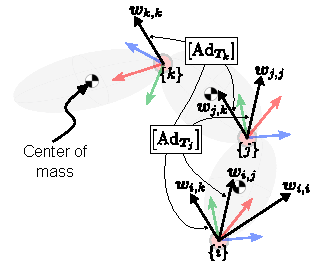
\includegraphics[width=0.5\textwidth]{wrench_propagation.pdf}
		\caption{\textbf{Wrench transmission.} Using the adjoint operator the wrenches at distal joints can be propagated backwards to proximal joints.}
		\label{fig:wrench_propagation}
	\end{center}
\end{figure}
% ---
The effect of all the distal wrenches to a joint $i$ can be aggregated via the matrix product of the corresponding adjoint operators. For example, the effect of wrench $\bm{w}_{k,k}$ in Fig.~\ref{fig:wrench_propagation} is propagated to joint $j$ as
%account for the effects of the wrenches in the distal links on the $i$-th link. The wrenches at joint $i$ resulting from the motion movements of the
%j’h link, these matrices can be
%cascaded as follows:
% ---
\begin{equation}
	\bm{w}_{i,k} = \underbrace{\left[\text{Ad}_{\bm{T}_{j}}\right]\left[\text{Ad}_{\bm{T}_{k}}\right]}_{\bm{U}_{i,k}}\bm{w}_{k,k} = \left[\text{Ad}_{\bm{T}_{j}}\right]\left[\text{Ad}_{\bm{T}_{k}}\right]\overbrace{\bm{A}_{k,k}}^{\bm{U}_{k,k}}\bm{\theta}_k.
	\label{eq:ext_wrench}
\end{equation}
% ---

Finally, the total wrench 

\begin{equation}
	\bm{w}_{j} = \bm{w}_{jj} + \sum_{k=j+1}^{N} \bm{w}_{jk} 
	\label{eq:wrench_link_i}
\end{equation}
% ---
at each of the joints can be expressed in matrix form
%For the simple 3 DOF manipulator in Fig.~\ref{fig:wrench_propagation}, this can be expressed in matrix form
%% ---
%\begin{equation}
%\begin{bmatrix}
%	\bm{w}_{i}\\
%	\bm{w}_{j}\\
%	\bm{w}_{k}
%\end{bmatrix} = 
%\begin{bmatrix}
%\bm{U}_{i,i} & \bm{U}_{i,j} & \bm{U}_{i,k}\\
%\bm{0} & \bm{U}_{j,j} & \bm{U}_{j,k}\\
%\bm{0} & \bm{0} & \bm{U}_{k,k}\\
%\end{bmatrix}¸
%\begin{bmatrix}
%	\bm{\theta}_{i}\\
%	\bm{\theta}_{j}\\
%	\bm{\theta}_{k}
%\end{bmatrix}
%\label{eq:wrench_inverse_dynamics}
%\end{equation}
%% ---
% ---
\begin{equation}
	\begin{bmatrix}
		\bm{w}_{i}\\
		\bm{w}_{j}\\
		\vdots \\
		\bm{w}_{n}
	\end{bmatrix} = 
	\begin{bmatrix}
		\bm{U}_{i,i} & \bm{U}_{i,j} & \cdots & \bm{U}_{i,k}\\
		\bm{0}       & \bm{U}_{j,j} & \cdots & \bm{U}_{j,n}\\
		\vdots       & \vdots       & \ddots & \vdots      \\
		\bm{0}       & \bm{0}       & \cdots & \bm{U}_{n,n}\\
	\end{bmatrix}
	\begin{bmatrix}
		\bm{\theta}_{i}\\
		\bm{\theta}_{j}\\
		\vdots \\
		\bm{\theta}_{n}
	\end{bmatrix}.
	\label{eq:wrench_inverse_dynamics}
\end{equation}
% ---
This expression corresponds to the inverse dynamics of the robot, that is, its output gives the $n$ wrenches necessary to produce the rigid body motions captured by the quantities ${}^\cframe{i}\bm{\omega}_i$ $,{}^\cframe{i}\dot{\bm{\omega}}_i$, and ${}^\cframe{i}\dot{\bm{v}}_i$ for each of the $n$ joints. Given that typically only joint torque $\tau$ is measured, Eq.~\eqref{eq:wrench_inverse_dynamics} is projected onto the rotation axes of the joints \cite{Siciliano2007SpringerHandbookRobotics} yielding
% ---
\begin{equation}\label{eq:lip_inverse_dnamics}
\bm{\tau} = \bm{Y}\left(
\bm{\omega},\dot{\bm{\omega}},\dot{\bm{v}}
;\bm{\lambda}\right)\bm{\theta} = \bm{Y}\left(\bm{q},\dot{\bm{q}},\ddot{\bm{q}};\bm{\lambda}\right)\bm{\theta}.
\end{equation}
%---
This expression for the inverse dynamics is linear in the parameters (LIP) $\bm{\theta}$ . The regressor matrix $\bm{Y}\left(\cdot\right)$ is dependent exclusively on the motion of the robot and its geometry $\bm{\lambda}$. The vector $\bm{\theta} \in \mathbb{R}^{10n}$ contains the stacked inertial parameters $\left\lbrace \bm{\theta}_i \right\rbrace^n_{i=1}$. The expression in Eq.~\eqref{eq:lip_inverse_dnamics} is equivalent to
%\begin{equation}
%	\bm{\tau} = \bm{M}\left(\bm{q};\bm{\theta}\right)\ddot{\bm{q}} + \bm{C}\left(\bm{q},\dot{\bm{q}};\bm{\theta}\right)\dot{\bm{q}} + \bm{g}\left(\bm{q};\bm{\theta}\right),
%\end{equation}
\begin{equation}
	\bm{\tau} = \bm{M}\left(\bm{q};\bm{\theta}\right)\ddot{\bm{q}} + \bm{c}\left(\bm{q},\dot{\bm{q}};\bm{\theta}\right) + \bm{g}\left(\bm{q};\bm{\theta}\right),
\end{equation}
% ---
where $\bm{M}(\cdot)$ is the configuration-dependent mass matrix of the robot, $\bm{c}(\cdot)$ is the vector of centrifugal and Coriolis torques, and $\bm{g}(\cdot)$ is the gravitational torque. 

\subsubsection{Estimation of the inertial parameters}

\paragraph*{Fixed base} The state of maturity of the research on inertial parameter identification for fixed base robots has lead to a rather standard procedure \cite{Swevers2007Dynamicmodelidentification}. Concretely, the process involves the generation of an excitation trajectory \cite{Gautier1992ExcitingTrajectoriesRobot,Park2006Fourierbasedoptimal} ---according to some observability index \redtext{REF}--- to collect $P$ measurement points $\left(\bm{\tau}{(k)},\bm{q}{(k)},\dot{\bm{q}}{(k)},\ddot{\bm{q}}{(k)}\right)$ representing instances of Eq.~\eqref{eq:lip_inverse_dnamics}. The estimation of the vector of inertial parameters $\bm{\theta}$ consists in using this set of points to solve the linear problem
% ---
\begin{equation}
	\bm{y} = \bm{F}\bm{\theta},
\end{equation}
% ---
where $\bm{y} = [\bm{\tau}^\intercal{(1)},\ldots,\bm{\tau}^\intercal(k),\ldots,\bm{\tau}^\intercal(P)]^\intercal \in \mathbb{R}^{nP}$ and $\bm{F} = [\bm{Y}_1^\intercal,\ldots,\bm{Y}_k^\intercal,\ldots,\bm{Y}_P^\intercal]^\intercal \in \mathbb{R}^{nP \times 10n}$. 
It is standard to follow a least-squares approach for the estimation of an optimal $\bm{\theta}$; i.e.
% ---
\begin{equation}
	\bm{\theta} = \left(\bm{F}^\intercal\bm{F}\right)^{-1}\bm{F}^\intercal\bm{y}.
\end{equation}
% ---
Methods to address the identifiability, numerical stability, and observability of the parameters have been discussed \cite{Siciliano2007SpringerHandbookRobotics}. For fixed base robots, specifically, it is known that some of the parameters of the links proximal to the base cannot be identified and methods to determine the base set of parameters have been developed \cite{Khalil2004Modelingidentificationcontrol}.


%More recently, the physical feasibility of the identified parameters has taken a prominent role \cite{Wensing2017Linearmatrixinequalities,Ayusawa2010Identificationstandardinertial,Traversaro2016Identificationfullyphysical,Sousa2014Physicalfeasibilityrobot}. This is vital due to its important in ensuring stable control methods. For instance, physically feasible inertial parameters lead to always invertible symmetric positive definite mass matrices. For the inertial parameters of a rigid body to be physically feasible, it is required that its mass is
%strictly positive and that its inertia matrix $ \bm{I}_i $ is symmetric positive definite (SPD)  with its eigenvalues ---$\lambda\left(\bm{I}_i\right) = [\lambda_1,\lambda_2,\lambda_3]^T$--- satisfying the triangle inequality, i.e.:\\
%%---
%\begin{equation}\label{eq:feasibility_constraints}
%	m_i>0, 
%	\quad
%		\bm{I}_i \succ 0,
%	\quad
%	\begin{aligned}
%		\begin{cases}
%				\lambda_1 + \lambda_2 \geq \lambda_3\\
%				\lambda_2 + \lambda_3 \geq \lambda_1\\
%				\lambda_1 + \lambda_3 \geq \lambda_2
%		\end{cases}
%	\end{aligned} 
%\end{equation}
%\begin{equation}\label{eq:feasibility_constraints}
%	m_i>0, 
%	\quad
%	\resizebox{0.4\hsize}{!}{$
%		\bm{I}_i=\begin{bmatrix}
%			XX_i & XY_i & XZ_i \\ XY_i & YY_i & YZ_i\\ XZ_i& YZ_i & ZZ_i
%		\end{bmatrix} \succ 0$},
%	\quad
%	\begin{aligned}
%		\resizebox{0.25\hsize}{!}{$\begin{cases}
%				\lambda_1 + \lambda_2 \geq \lambda_3\\
%				\lambda_2 + \lambda_3 \geq \lambda_1\\
%				\lambda_1 + \lambda_3 \geq \lambda_2
%			\end{cases}$}
%	\end{aligned} 
%\end{equation}
%---

%the mass must be strictly positive $m>0$ and its inertia matrix $\bm{I}$ ought to be symmetric positive definite. 




%Various methods have been proposed for estimating the inertial parameters of humanoid and legged robots. For example, methods that use the base-link dynamics, requiring only the generalized coordinates of the base-link, joint angles, and external forces have been developed \cite{Ayusawa2008Identificationhumanoidrobots,Ayusawa2008Identificationinertialparameters,Ayusawa2009MinimalsetInertial,Iwasaki2012Identificationinertialparameters}. The work in \cite{Jovic2016HumanoidHumanInertia} introduced a hierarchical optimization approach that accurately reconstructs ground reaction forces and force moments. A method was proposed in \cite{Mistry2009Inertialparameterestimation} for whole body inertial parameter estimation using a partial force sensor set that demonstrated the feasibility of inertial parameter estimation for floating-base humanoid systems. A state-estimation technique for legged robots that combines forward kinematic and preintegrated contact factors was introduced in \cite{Hartley2018LeggedRobotState}. A more recent study \cite{Ayusawa2014Identifiabilityidentificationinertial} addressed the dynamics of legged systems and proposed a method for identifying inertial parameters based on the underactuated base-link dynamics. Buchanan et al. \cite{RussellBuchanan2021LearningInertialOdometry} has introduced a proprioceptive state estimator for legged robots based on a learned displacement measurement from IMU data, which significantly reduces drift in challenging scenarios. Extensions for floating base robots with flexible joints and links have been presented elsewhere \cite{Khalil2017GeneralDynamicAlgorithm}}.


%Several methods have been proposed to estimate the inertial parameters of humanoid and legged robots. For instance, there are methods utilizing base-link dynamics, which require generalized coordinates of the base-link, joint angles, and external forces \cite{Ayusawa2008Identificationhumanoidrobots, Ayusawa2008Identificationinertialparameters, Ayusawa2009MinimalsetInertial, Iwasaki2012Identificationinertialparameters}. The work by Jovic et al. \cite{Jovic2016HumanoidHumanInertia} introduced a hierarchical optimization approach, accurately reconstructing ground reaction forces and force moments. Mistry et al. \cite{Mistry2009Inertialparameterestimation} proposed a method for whole-body inertial parameter estimation, demonstrating feasibility for floating-base humanoid systems using a partial force sensor set. Another state-estimation technique for legged robots, combining forward kinematics and preintegrated contact factors, was introduced by Hartley et al. \cite{Hartley2018LeggedRobotState}. Addressing the dynamics of legged systems, Ayusawa et al. \cite{Ayusawa2014Identifiabilityidentificationinertial} proposed a method based on underactuated base-link dynamics for identifying inertial parameters. Buchanan et al. \cite{RussellBuchanan2021LearningInertialOdometry} introduced a proprioceptive state estimator for legged robots based on learned displacement measurement from IMU data, significantly reducing drift in challenging scenarios. Extensions for floating-base robots with flexible joints and links have been presented elsewhere \cite{Khalil2017GeneralDynamicAlgorithm}. In general, unlike the methods for the inertial parameter estimation of fixed based robots, the methods for floating base robots are not as standardized.

\paragraph*{Floating base} Research in robotics is actively exploring methods for estimating the inertial parameters of floating base systems; in particular, humanoid and legged robots. For instance, there are methods utilizing base-link dynamics, which require generalized coordinates of the base-link, joint angles, and external forces \cite{Ayusawa2008Identificationhumanoidrobots, Ayusawa2008Identificationinertialparameters, Ayusawa2009MinimalsetInertial, Iwasaki2012Identificationinertialparameters}. The work by Jovic et al. \cite{Jovic2016HumanoidHumanInertia} introduced a hierarchical optimization approach, accurately reconstructing ground reaction forces and force moments. Mistry et al. \cite{Mistry2009Inertialparameterestimation} proposed a method for whole-body inertial parameter estimation, demonstrating feasibility for floating-base humanoid systems using a partial force sensor set. Another state-estimation technique for legged robots, combining forward kinematics and preintegrated contact factors, was introduced by Hartley et al. \cite{Hartley2018LeggedRobotState}. Addressing the dynamics of legged systems, Ayusawa et al. \cite{Ayusawa2014Identifiabilityidentificationinertial} proposed a method based on underactuated base-link dynamics for identifying inertial parameters. Buchanan et al. \cite{RussellBuchanan2021LearningInertialOdometry} introduced a proprioceptive state estimator for legged robots based on learned displacement measurement from IMU data, significantly reducing drift in challenging scenarios. Extensions for floating-base robots with flexible joints and links have been presented elsewhere \cite{Khalil2017GeneralDynamicAlgorithm}. In general, unlike the methods for the inertial parameter estimation of fixed based robots, the methods for floating base robots are not as standardized.

% SUBSECTION ========================================================================================
\subsection{Physical feasibility of the inertial parameters}\label{sec:spd_manifold}
%A \emph{differentiable manifold} $\mathcal{M}$ is a topological space that is locally similar to Euclidean space and has a globally defined differential structure \cite{Jayasumana2013KernelmethodsRiemannian}. $\mathcal{T}_{\bm{P}}\mathcal{M}$ is the \emph{tangent space} at a point $\bm{P}\in \mathcal{M}$ and represents the vector space of all the possible tangent vectors to the manifold that pass through $\bm{P}$. The pair $(\mathcal{M},\rho)$ defines a \emph{Riemannian manifold} if $ \mathcal{M} $ is differentiable and is equipped with a positive definite metric tensor $\rho$ at each point \cite{Pennec2006Riemannianframeworktensor}. 
More recently, the physical feasibility of the identified parameters has taken a prominent role \cite{Wensing2017Linearmatrixinequalities,Ayusawa2010Identificationstandardinertial,Traversaro2016Identificationfullyphysical,Sousa2014Physicalfeasibilityrobot}. This is vital due to its importance in ensuring stable control methods. For instance, physically feasible inertial parameters lead to always invertible symmetric positive definite mass matrices. For the inertial parameters of a rigid body to be physically feasible, it is required that its mass is
strictly positive and that its inertia matrix $ \bm{I}_i $ is symmetric positive definite (SPD)  with its eigenvalues ---$\bm{s}\left(\bm{I}_i\right) = [s_1,s_2,s_3]^T$--- satisfying the triangle inequality, i.e.:\\
%---
\begin{equation}\label{eq:feasibility_constraints}
	m_i>0, 
	\quad
	\bm{I}_i \succ 0,
	\quad
	\begin{aligned}
		\begin{cases}
			s_1 + s_2 \geq s_3\\
			s_2 + s_3 \geq s_1\\
			s_1 + s_3 \geq s_2
		\end{cases}
	\end{aligned} 
\end{equation}
% ---

The physical feasibility constraints can be expressed in the language of differential geometry. First, it is necessary to define a differentiable manifold $\mathcal{M}$. It is a topological space that exhibits local similarity to Euclidean space and possesses a globally defined differential structure \cite{Jayasumana2013KernelmethodsRiemannian}. At any point $\bm{P}$ on the manifold there is an associated tangent space, denoted as $\mathcal{T}_{\bm{P}}\mathcal{M}$, that encompasses the vector space containing all possible tangent vectors to $\mathcal{M}$ that pass through $\bm{P}$. A Riemannian manifold is defined by the pair $(\mathcal{M},\rho)$, where each point $\bm{P}$ in $\mathcal{M}$ is equipped with a positive definite metric tensor $\rho$ \cite{Pennec2006Riemannianframeworktensor}.

%A differentiable manifold, denoted as $\mathcal{M}$, is a topological space that exhibits local similarity to Euclidean space and possesses a globally defined differential structure \cite{Jayasumana2013KernelmethodsRiemannian}. The tangent space at a point $\bm{P}$ in $\mathcal{M}$, denoted as $\mathcal{T}_{\bm{P}}\mathcal{M}$, encompasses the vector space containing all possible tangent vectors to the manifold that pass through $\bm{P}$. A Riemannian manifold is defined by the pair $(\mathcal{M},\rho)$, where $\mathcal{M}$ is a differentiable manifold and each point in $\mathcal{M}$ is equipped with a positive definite metric tensor $\rho$ \cite{Pennec2006Riemannianframeworktensor}.

%Denoting $\mathcal{S}^n \triangleq\left\lbrace \bm{S} \in \mathbb{R}^{n \times n} : \bm{S} = \bm{S}^T\right\rbrace$ as the space of real square symmetric matrices of dimension $n \times n$. Then, the space of $n \times n$ SPD matrices $ \mathcal{S}^n_{++}\triangleq \left\lbrace \bm{P}\in \mathcal{S}^n : \bm{P} \succ 0 \right\rbrace $  defines a smooth submanifold $\mathcal{M}$ of $\mathcal{S}^n$. By definition, its tangent space $\mathcal{T}\mathcal{M} \in \mathcal{S}^n$ is equipped with an \emph{affine invariant Riemannian metric} $\rho$ \cite{Lee2018geometricalgorithmrobust}. Consequently, $ \mathcal{S}^n_{++} $ defines a Riemannian manifold. Finally, the product manifold $ \mathcal{M}^N $ of SPD manifolds is the Cartesian product $\mathcal{M}^N =\mathcal{M}_1\times \mathcal{M}_2\times \ldots \times \mathcal{M}_N$. It is the set of matrices  $\left\lbrace \left(\bm{P}_1,\ldots,\bm{P}_N\right):\bm{P}_i\in\mathcal{M}_i,\quad i=1,\ldots,N\right\rbrace$ and is also a Riemannian manifold with the metric $ \bm{\rho} =\text{diag}\left( \rho_{1},\ldots, \rho_{N} \right) $. %Similarly, the generalizations of the operators mentioned above to $\mathcal{M}^N$ are the concatenations of the individual operators for each $\mathcal{M}_i$.

The inertial parameters of rigid body, and by extension of a robot, are associated to the manifolds of SPD matrices. To make clear this relation, let $\mathcal{S}^n$ be the space of real square symmetric matrices with dimension $n \times n$, denoted as $\mathcal{S}^n \triangleq\left\lbrace \bm{S} \in \mathbb{R}^{n \times n} : \bm{S} = \bm{S}^T\right\rbrace$. The space of $n \times n$ SPD matrices, $\mathcal{S}^n_{++}\triangleq \left\lbrace \bm{P}\in \mathcal{S}^n : \bm{P} \succ 0 \right\rbrace$, defines a smooth submanifold $\mathcal{M}$ within $\mathcal{S}^n$. Its tangent space $\mathcal{T}\mathcal{M} \in \mathcal{S}^n$ is equipped with an \emph{affine invariant Riemannian metric} $\rho$ \cite{Lee2018geometricalgorithmrobust}, thereby making $ \mathcal{S}^n_{++} $ a Riemannian manifold. Finally, the Cartesian product $\mathcal{M}^N =\mathcal{M}_1\times \mathcal{M}_2\times \ldots \times \mathcal{M}_N$ defines the product manifold of SPD manifolds.  It represents the set of matrices $\left\lbrace \left(\bm{P}_1,\ldots,\bm{P}_N\right):\bm{P}_i\in\mathcal{M}_i,\quad i=1,\ldots,N\right\rbrace$ and is also a Riemannian manifold with the metric $ \bm{\rho} =\text{diag}\left( \rho{1},\ldots, \rho{N} \right) $. The physical feasibility constraints of the inertial parameters $\bm{\theta}_i$ of the $i$-th link, summarized in Eq.~\eqref{eq:feasibility_constraints}, are satisfied if the pseudo inertia matrix 
%---
%\begin{equation}\label{eq:pseudo_inertia_matrix}
%\bm{P}_i(\bm{\theta}_i)=f(\bm{\theta}_i)=\begin{bmatrix}
%	\bm{\Sigma}_i && \bm{h} \\ \bm{h}^T && m
%\end{bmatrix} \in \mathcal{S}^4,
%\end{equation}
\begin{equation}\label{eq:pseudo_inertia_matrix}
	\bm{P}_i(\bm{\theta}_i)=f(\bm{\theta}_i)=\begin{bmatrix}
		\frac{1}{2}\text{tr}(\bm{I}_i)\mathbb{1} - \bm{I}_i && \bm{h} \\ \bm{h}^T && m
	\end{bmatrix} \in \mathcal{S}^4,
\end{equation}
%---
defined for each rigid body is symmetric positive-definite \cite{Wensing2017Linearmatrixinequalities}; that is, $\bm{P}_i(\bm{\theta}_i)\in \mathcal{S}_{++}^4$. Note that $\mathbb{1}$ is used to denote the $3 \times 3$ identity matrix. %Here $ \bm{\Sigma}_i = \frac{1}{2}\text{tr}(\bm{I}_i)\mathbb{1} - \bm{I}_i\in \mathcal{S}^3 $ is called the \emph{density weighted covariance matrix}. Conversely,  $ \bm{I}_i = \text{tr}\left(\bm{\Sigma}_i\right)\mathbb{1} - \bm{\Sigma}_i \in \mathcal{S}^3_{++} $, where $\mathbb{1}$ is the $3 \times 3$ identity matrix. 
The requirement that $\bm{P}_i(\bm{\theta}_i) \succ 0$ implies the fully physically feasible inertial parameters are in the manifold $\mathcal{S}^4_{++}=\left\lbrace \bm{P}_i(\bm{\theta}_i) \in \mathcal{S}^{4}: \bm{P}_i(\bm{\theta}_i) \succ 0 \right\rbrace$. For every rigid body $i$ in the kinematic chain, there exist a pseudo inertia matrix  \cite{Lee2018geometricalgorithmrobust}. Consequently, this means that the inertial parameters of a robot define a point $\left\lbrace \bm{P}_i\right\rbrace_{i=1}^N$ in the Riemannian product manifold $\mathcal{M}^N$.


%\TODO
%\redtext{Research in robotics is actively exploring methods for estimating the inertial parameters of floating base robots. Various innovative approaches have been developed to accurately determine the inertial properties of these systems. Legged robots equipped with Inertial Measurement Units (IMUs) in their pelvis link can leverage gyroscopes and accelerometers to estimate the orientation of the floating base with respect to an external frame. Another approach \cite{Mistry2009Inertialparameterestimation} involves partial force sensing, demonstrating the feasibility of inertial parameter estimation for floating-base humanoid systems. A model-free approach has been introduced for precise control of humanoid robot joints, incorporating an input-output online identification procedure to estimate inertial parameters. Additionally, a proprioceptive base estimator for humanoid robots has been developed using extended Kalman filtering on matrix Lie groups, focusing on estimating IMU biases, floating base, and feet positions. These diverse methods showcase the ingenuity applied to address the unique challenges associated with estimating inertial parameters in floating-base legged robots, considering their complex dynamics and locomotion intricacies. Extension for floating base robots with flexible joints and links have been presented elsewhere \cite{Khalil2017GeneralDynamicAlgorithm}}
%Research in robotics is actively exploring methods for estimating the inertial parameters of floating base robots. Various innovative approaches have been developed to accurately determine the inertial properties of these systems. One notable method involves an iterative primitive shape division, presented in a research paper, for the inertia parameter identification of floating-base robots. Legged robots equipped with Inertial Measurement Units (IMUs) in their pelvis link can leverage gyroscopes and accelerometers to estimate the orientation of the floating base with respect to an external frame, employing techniques such as integration of angular velocities and the use of Kalman or complementary filters. Another approach involves partial force sensing, demonstrating the feasibility of inertial parameter estimation for floating-base humanoid systems. This method has been successfully applied to both simulated bipedal humanoid robots and real robot dogs navigating challenging terrains. A model-free approach has been introduced for precise control of humanoid robot joints, incorporating an input-output online identification procedure to estimate inertial parameters. Additionally, a proprioceptive base estimator for humanoid robots has been developed using extended Kalman filtering on matrix Lie groups, focusing on estimating IMU biases, floating base, and feet positions. These diverse methods showcase the ingenuity applied to address the unique challenges associated with estimating inertial parameters in floating-base legged robots, considering their complex dynamics and locomotion intricacies. \redtext{Extension for floating base robots with flexible joints and links have been presented elsewhere \cite{Khalil2017GeneralDynamicAlgorithm}}


%\hrule
%, Af is a 6 X 10 matrix,
%and Oi is the vector of the ten unknown inertial pa-
%rameters.
%according to Newton's third law. As a result, the dynamic parameters of link $i$ inside an open kineto-dynamic chain will include:
%\begin{itemize}
%	\item $m_i$: the mass of link $i$
%	\item $\bm{I}^{CoM}_i$: the inertia matrix of link $i$, calculated with respect to the center of mass of the link
%	\item $\bm{I}_i$: the inertia matrix of link $i$, calculated with respect to the joint frame
%	\item $\bm{g}$: the gravitational force vector
%\end{itemize}
%
%
%• fc the acting force exerted by joint i on link i;
%• —fi+i\ the reacting force exerted by joint i + 1 on link i;
%• Tii the acting torque exerted by joint i on link i;
%• — Tj+i: the reacting torque exerted by joint i + l o n link i.
%
%
%%By default, all dynamic parameters are expressed with respect to the
%%common reference frame (frame 0).  A well-known result, the parallel-axis theorem, is one way
%%of computing how the inertia tensor changes under translations of the reference
%%coordinate system. 
%
%
% 
%% 
%
%
%
%
%
%\subsubsection{Something}
%Let $\bm{\omega} = \begin{bmatrix}\omega_x & \omega_y & \omega_z \end{bmatrix}^\intercal$ represent any real vector in $\mathbb{R}^3$ and let $vec(\cdot)$ indicate the vectorization of a matrix; then, the terms in equations (\ref{eq:self_wrench}) and (\ref{eq:ext_wrench}) are defined as follows:
%%\begin{multicols}{2}
%\begin{equation*}
%	\bm{I}_{i,vec} = [XX_i, XY_i , XZ_i , YY_I , YZ_i , ZZ_i ]
%\end{equation*}
%\begin{equation*}
%	\bar{\bm{I}_i}= \begin{bmatrix}
%		\bm{I}_{i,vec}               & \bm{0}_{1\times6} & \bm{0}_{1\times6}\\
%		\bm{0}_{1\times6} & \bm{I}_{i,vec}               & \bm{0}_{1\times6}\\
%		\bm{0}_{1\times6} & \bm{0}_{1\times6} & \bm{I}_{i,vec}
%	\end{bmatrix}
%\end{equation*}
%\begin{equation*}
%	\bm{mC}_i = \begin{bmatrix}
%		mX_i & mY_i & mZ_i
%	\end{bmatrix}^\intercal
%\end{equation*}
%\begin{equation*}
%	\tilde{\bm{mC}_i}= \begin{bmatrix}
%		\bm{mC}_i^\intercal              & \bm{0}_{1\times3} & \bm{0}_{1\times3}\\
%		\bm{0}_{1\times3} & \bm{mC}_i^\intercal              & \bm{0}_{1\times3}\\
%		\bm{0}_{1\times3} & \bm{0}_{1\times3} & \bm{mC}_i^\intercal
%	\end{bmatrix}
%\end{equation*}
%
%\begin{equation*}
%	\tilde{\bm{\omega}}=vec([\bm{\omega} \times]^\intercal[\bm{\omega} \times]^\intercal)
%\end{equation*}
%\begin{equation*}
%	\bar{\bm{\omega}}=vec([\bullet \bm{\omega}]^\intercal[\bm{\omega} \times]^\intercal)
%\end{equation*}
%
%\subsubsection{Identification of the inertial parameters}



%\begin{equation}
%	\prescript{}{q}{\bm{n}}_i = \bm{n}_{i} + \left[\bm{f}_{ii}\right]\bm{c}_i =  
%\end{equation}

%bsection{Basics of robot system identification}
%bsubsection{Kinematic calibration}
%bsubsection{Inertial parameter identification}
% For fixed based robots
% For floating base robots



% ===========================================================================================
%                                           |                                               |
% -------------------------------------- SECTION -------------------------------------------|
%                                           |                                               |
% ===========================================================================================


%\subsection{Some context}
%\redtext{\say{The body schema is viewed as a set of fronto-parietal networks that integrate information originating from regions of the body and external space in a way that is functionally relevant to specific actions performed by different body parts$\ldots$ It represents the body's spatial properties, including the length of limbs and limb segments, their arrangement, the configuration of the segments in space, and the shape of the body surface$\ldots$ The body schema is characterized by short-term plasticity and reorganization, as shown by the quick integration of tools into the body schema}} \cite{Morasso2015Revisitingbodyschema}

% ===========================================================================================
%                                           |                                               |
% -------------------------------------- SECTION -------------------------------------------|
%                                           |                                               |
% ===========================================================================================
\section{Describing body shape: Connectivity and graph theory}

%As discussed in \cite{Featherstone2007RigidBodyDynamics}, the connectivity of a kinematic chain describes how its parts are connected to each other. This is known as the mechanical topology; i.e., the arrangement of joints and links. \redtext{The topology is a fundamental piece of knowledge to describe the body structure. Without it, the individual geometry of the parts lacks meaning. Similarly, knowledge of the inertial properties of each of the bodies in a kinematic chain is insufficient to understand the dynamics associated to their coupling. Thus, a robotic agent must be capable of inferring the topology of its body before it can instantiate its kinematic and dynamic properties.}
As outlined by Featherstone \cite{Featherstone2007RigidBodyDynamics}, the connectivity of a kinematic chain delineates the interconnection of its components, constituting what is known as the mechanical topology---essentially, the configuration of joints and links. Understanding this topology is crucial as it serves as a foundational element for describing the body structure. Without this information, the individual geometry of the components lacks significance. Similarly, knowledge of only the inertial properties of each body in a kinematic chain is insufficient for describing the dynamics associated with their coupling. Therefore, a robotic agent must possess the capability to deduce the topology of its body before instantiating its kinematic and dynamic properties.

Having the topology of the body such relevance, the fact is that a scarce number of works have pondered the problem of how to learn it (see, for example, \cite{Bongard2006Resilientmachinescontinuous}). It seems reasonable to assume that the this stems from the typical premise that this information is known a priori. Yet, a fully independent robotic agent that is to develop an understanding of its body through the development of a body schema needs to obtain this information exclusively by itself. This gains prominence as gradually robots become more adaptable and modular. Therefore, if there is access to the number and modalities of the robot's sensorimotor signals, an indication of the body topology must be extracted from them. But, how?

\subsection{Embodiment and information structure}\label{sec:embodiment_and_information}
%To find an answer to the question of how to learn the body topology, this dissertation shares the well-accepted hypothesis that the interaction of an agent with its environment and its body morphology induce statistical regularities in its sensorimotor signals \cite{Pfeifer2006InformationTheoreticImplications,Pfeifer2007SelfOrganizationEmbodiment,LungarellaEmbodimentInformationCausal,Pfeifer2006Howbodyshapes}, see Fig.~\ref{fig:implications_of_embodiment}. 
%% ---
%\begin{figure}[t!]
%	\begin{center}
%		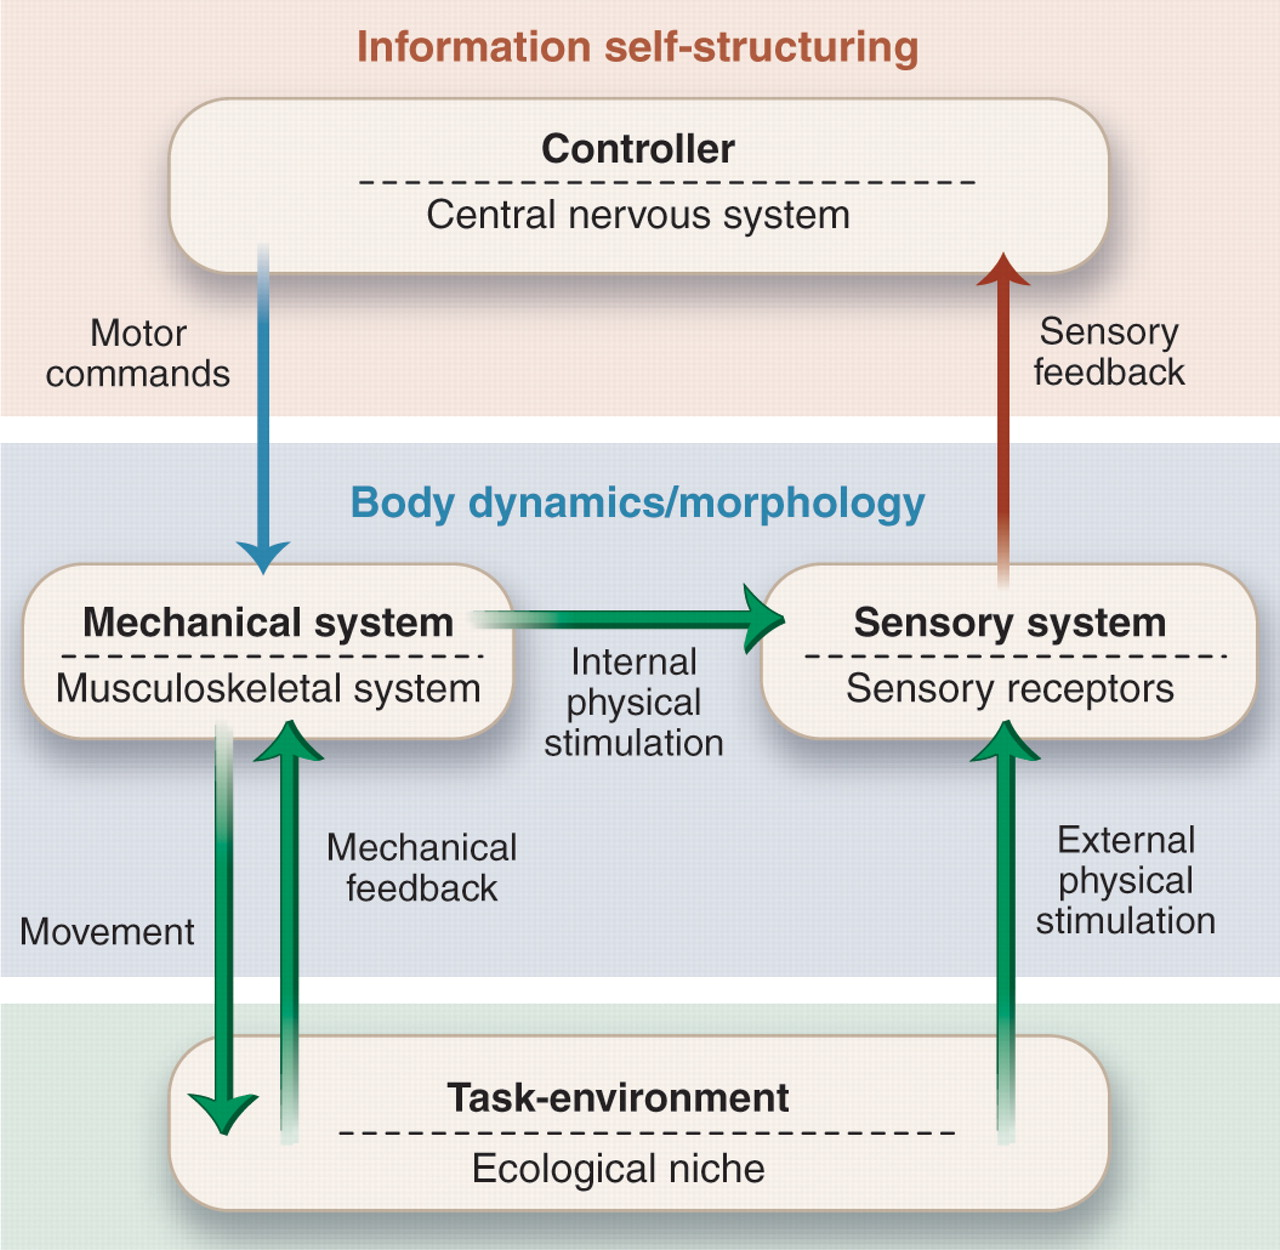
\includegraphics[width=0.7\textwidth]{implications_of_embodiment}
%		\caption{\textbf{Implications of embodiment.} From Pfeifer et al. \cite{Pfeifer2007SelfOrganizationEmbodiment}. Reprinted with permission from AAAS.}
%		\label{fig:implications_of_embodiment}
%	\end{center}
%\end{figure}
%% ---
%
%These statistical regularities, connected to the concept of sensorimotor contingencies \cite{Jacquey2019Sensorimotorcontingenciesas}, have been captured using information-theoretic quantities, which measure the information between the different modalities in the robot's sensorimotor system \cite{Schmidt2013Bootstrappingperceptionusing,Lungarella2006Mappinginformationflow,Polani2009Modelsinformationprocessing,Bossomaier2016introductiontransferentropy,Olsson2006unknownsensorsactuators}. Fig.~\ref{fig:emobodiment_and_info_structure} illustrates how information structure in the sensorimotor signals can result from embodiment. It shows a number of bodies equipped with a set of sensors (Fig.~\ref{fig:f1a_embodiment_and_information_structure}). These sensors can be considered information sources that have a relationship tied to information sharing with each other. The strength of these relationships is visually represented by the blue lines (edges) connecting the sensors. Due to the morphology of the robot, stronger connections exist between certain sensors---represented by dark blue edges. These strong connections indicate the body topology of the robot, depicted in Fig.~\ref{fig:f1b_embodiment_and_information_structure}, which is a tree-like structure where the strongest sharing of information  occurs between sensors in adjacent bodies. The main message of this example is that the structure of the robot's body becomes a hypothesis for the strength of information sharing.
%\hrule
% ---
\begin{figure}[t!]
	\begin{center}
		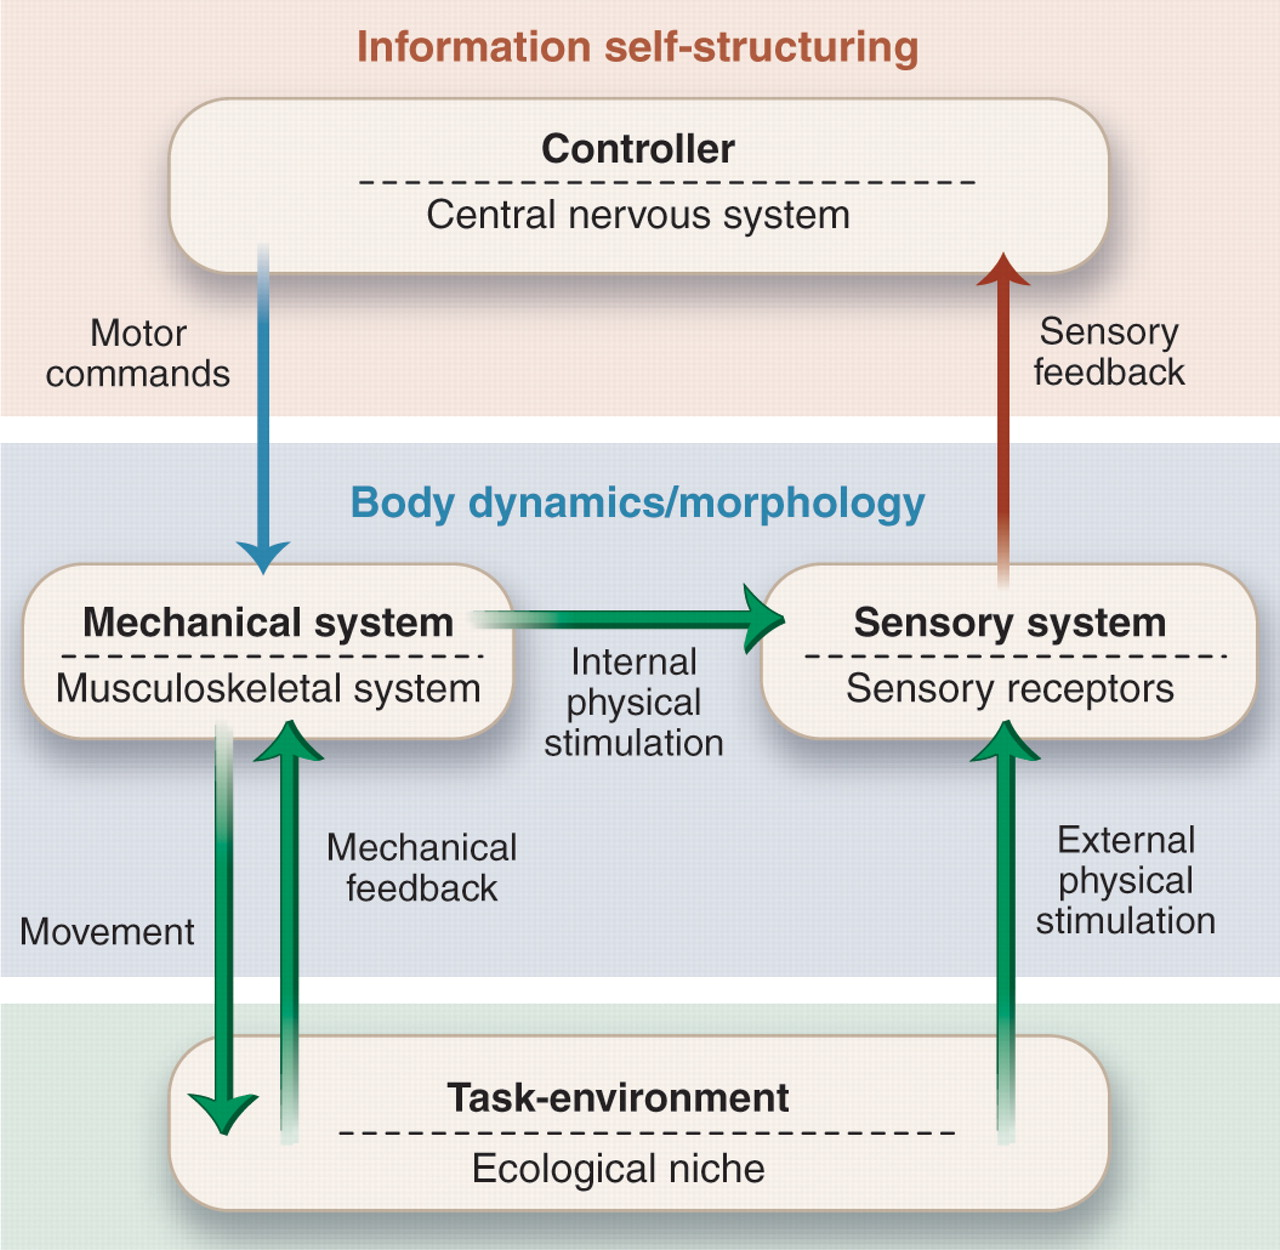
\includegraphics[width=0.5\textwidth]{implications_of_embodiment}
		\caption{\textbf{Implications of embodiment.} From Pfeifer et al. \cite{Pfeifer2007SelfOrganizationEmbodiment}. Reprinted with permission from AAAS.}
		\label{fig:implications_of_embodiment}
	\end{center}
\end{figure}
% ---
To address the question of how the body's topology can be learned, this dissertation relies on the widely accepted hypothesis that an agent's interaction with its environment and its body morphology gives rise to statistical regularities in its sensorimotor signals \cite{Pfeifer2006InformationTheoreticImplications,Pfeifer2007SelfOrganizationEmbodiment,LungarellaEmbodimentInformationCausal,Pfeifer2006Howbodyshapes} (see Fig.~\ref{fig:implications_of_embodiment}). These statistical regularities, intertwined with the concept of sensorimotor contingencies \cite{Jacquey2019Sensorimotorcontingenciesas}, have been quantified using information-theoretic measures, which assess the information sharing among different modalities in the robot's sensorimotor system \cite{Schmidt2013Bootstrappingperceptionusing,Lungarella2006Mappinginformationflow,Polani2009Modelsinformationprocessing,Bossomaier2016introductiontransferentropy,Olsson2006unknownsensorsactuators}. 
% ---
\begin{figure*}[!t]
	\centering	
	\hspace*{\fill}
	\begin{subfigure}[t]{0.40\textwidth}
		\subcaption{}
		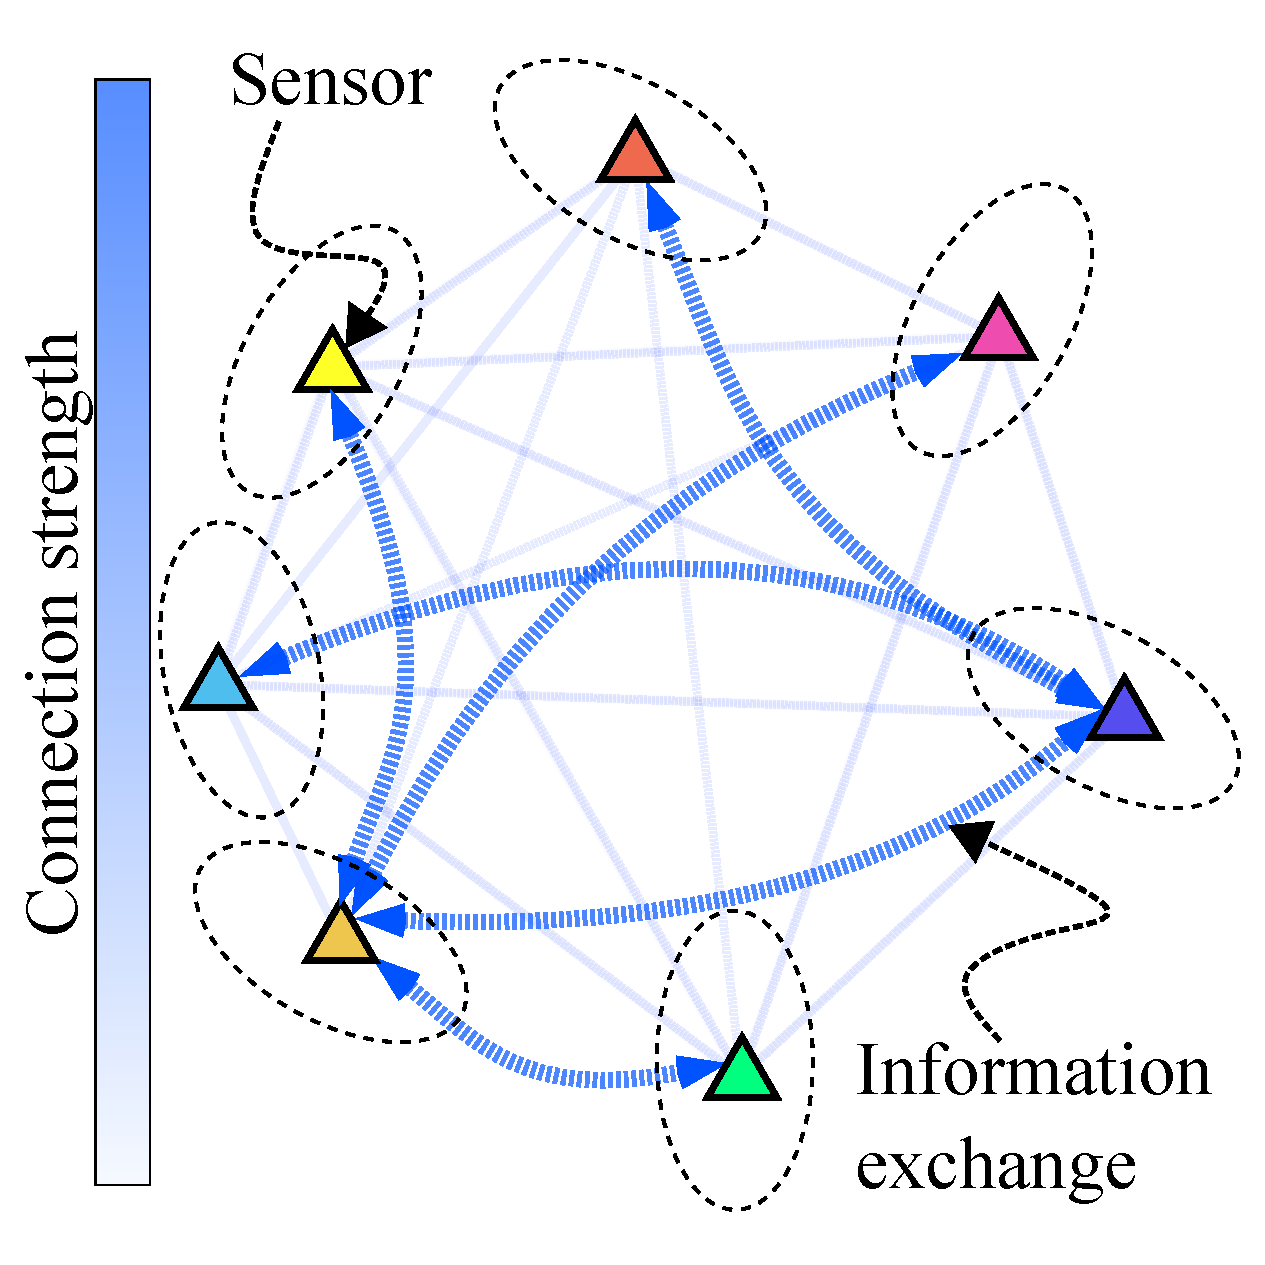
\includegraphics[width=\textwidth]{f1a_embodiment_and_information_structure.pdf}
		\label{fig:f1a_embodiment_and_information_structure}
	\end{subfigure}	
	\hfill
	\begin{subfigure}[t]{0.40\textwidth}
		\subcaption{}
		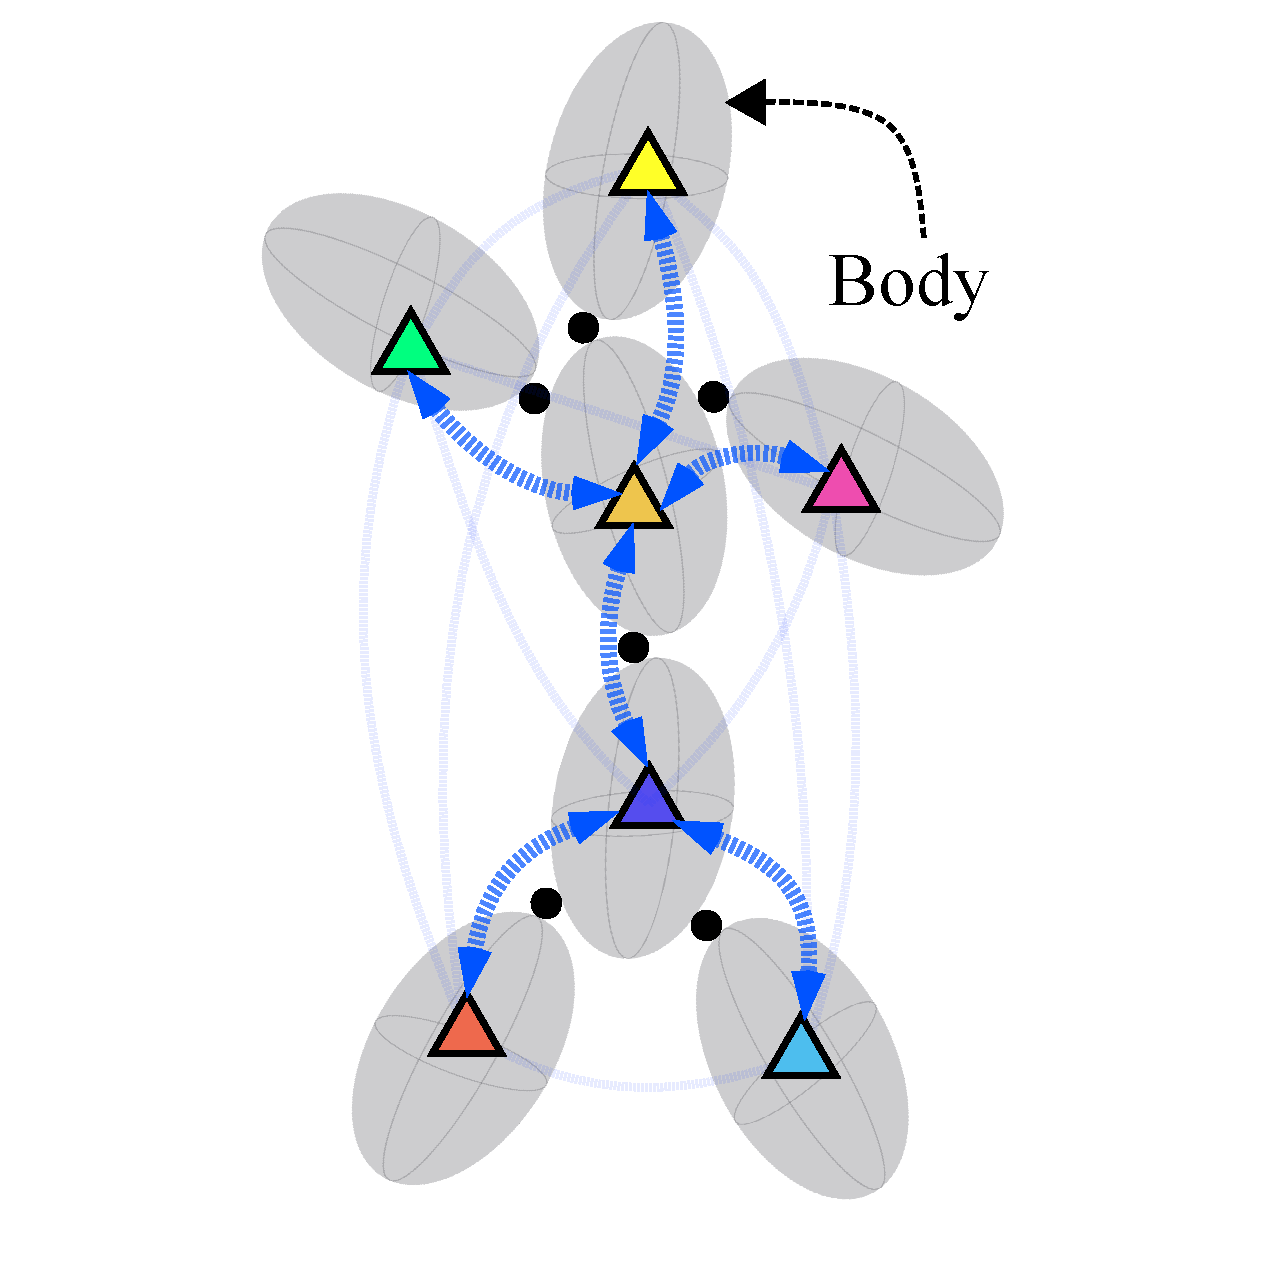
\includegraphics[width=\textwidth]{f1b_embodiment_and_information_structure.pdf}
		\label{fig:f1b_embodiment_and_information_structure}
	\end{subfigure}	
	\hspace*{\fill}
	\caption{\label{fig:emobodiment_and_info_structure} \textbf{Embodiment and information structure.} (\subref{fig:f1a_embodiment_and_information_structure}) Sensors on a robot exchange information at different strength levels. (\subref{fig:f1b_embodiment_and_information_structure}) This strength is associated with the embodiment of the robot, a kinematic tree in this case.}
\end{figure*}
% ---

Fig.~\ref{fig:emobodiment_and_info_structure} illustrates how information structure in sensorimotor signals can emerge from embodiment. It depicts various bodies equipped with sensors (Fig.~\ref{fig:f1a_embodiment_and_information_structure}), with these sensors acting as information sources having relationships that involve sharing information. The strength of these relationships is visually denoted by the blue lines (edges) connecting the sensors. Owing to the robot's morphology, stronger connections exist between specific sensors, as indicated by dark blue edges. These robust connections signify the body topology of the robot, illustrated in Fig.~\ref{fig:f1b_embodiment_and_information_structure}, portraying a tree-like structure where the most substantial information sharing occurs between sensors in adjacent bodies. The key takeaway from this example is that the structure of the robot's body serves as a hypothesis for the strength of information sharing.



%The embodiment of a robot determines its perceptual and behavioral capabilities and influences the emergence of sensorimotor regularities arising from body-environment interaction\cite{Pfeifer2006Howbodyshapes}. Information-theoretic quantities have been used to capture these regularities as information flows between the various modalities in the sensorimotor system\cite{Schmidt2013Bootstrappingperceptionusing,Lungarella2006Mappinginformationflow,Polani2009Modelsinformationprocessing,Bossomaier2016introductiontransferentropy,Olsson2006unknownsensorsactuators}. To illustrate how embodiment influences information structure, consider a hypothetical robot equipped with a set of sensors, depicted on Fig.~\ref{fig:f1a_embodiment_and_information_structure}. From an information-theoretic perspective, these sensors are information sources that share information with each other. The strength of these relations is represented graphically as edges connecting the sensors (light blue edges). As a result of the underlying embodiment of the robot, stronger connections between sensors exist (dark blue edges). These strong connections hint at the robot's body topology (Fig.~\ref{fig:f1b_embodiment_and_information_structure}), a tree-like serial kinematic structure where the stronger exchange of information occurs between sensors of adjacent bodies. Succinctly, body structure becomes the hypothesis behind the strength of information sharing. 


\subsection{Fundamentals of graph theory}
The sensorimotor relationships shown in Fig.~\ref{fig:emobodiment_and_info_structure} are an example of mathematical object known as a graph \cite{West2001Introductiongraphtheory}. The mechanical topology of a robot can also be represented as a graph, whose connectivity represents the topology \cite{Featherstone2007RigidBodyDynamics}. Therefore, it is important to introduce some fundamental concepts related to graph theory before proceeding with the discussion. 

\subsubsection{Definition of a graph}
A graph $\mathcal{G} = \left(\mathcal{V}, \mathcal{E}\right)$ is a mathematical construct the represents the interconnections between the elements of a system \cite{West2001Introductiongraphtheory}. These elements are represented as a set $ \mathcal{V}=\left\lbrace v_i\right\rbrace^n_{i=1}$ of $n$ \emph{nodes} (also called \emph{vertices}) and their connections are depicted as a set of \emph{edges} $ \mathcal{E}= \left\lbrace e_i\right\rbrace^m_{i=1} \subseteq \mathcal{V} \times \mathcal{V} $. Note that it is possible that an edge connects a node to itself, in which case the edge defines a self loop.
% ---
%\begin{figure}[th!]
%	\begin{center}
	%		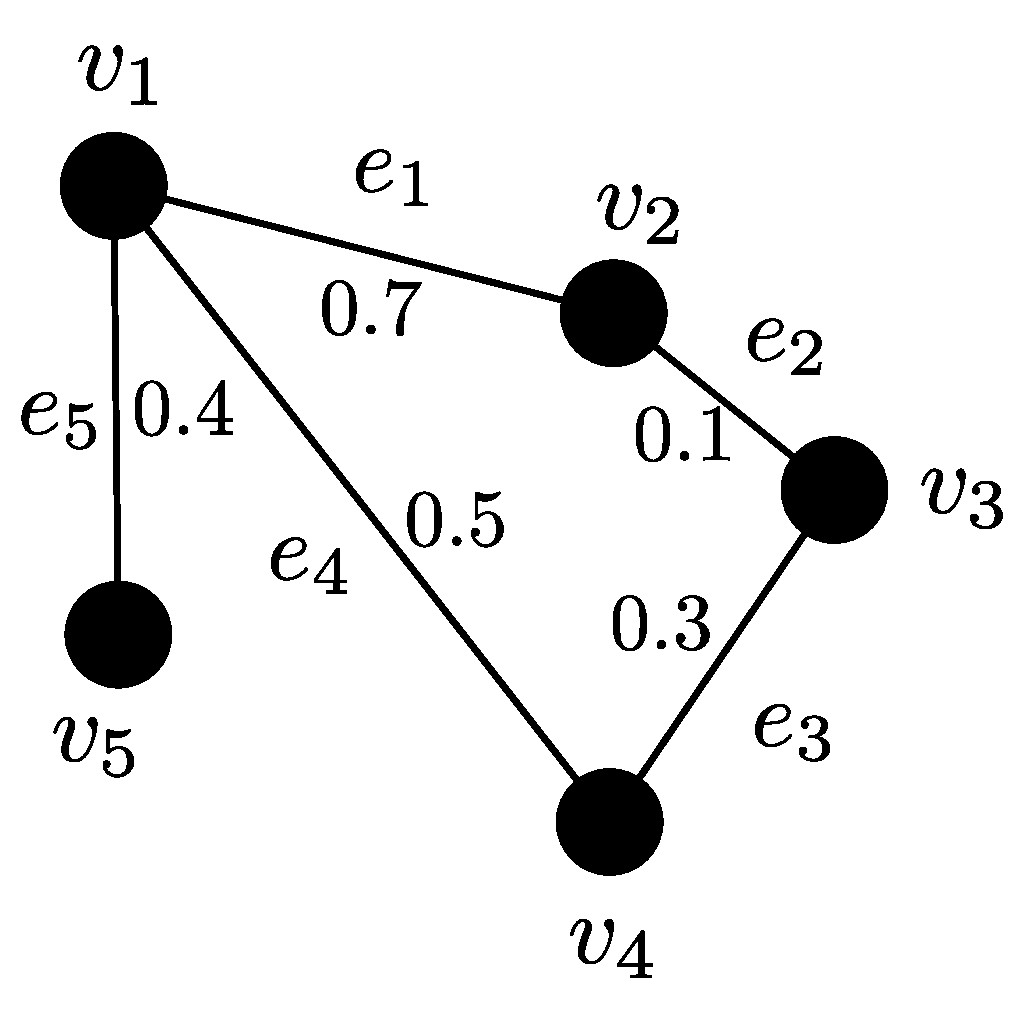
\includegraphics[width=0.5\textwidth]{example_graph.pdf}
	%		\caption{Example graph.}
	%		\label{fig:example_graph}
	%	\end{center}
%\end{figure}
% ---
\begin{figure*}[!h]
	\centering	
	\hspace*{\fill}
	\begin{subfigure}[t]{0.32\textwidth}
		\subcaption{}
		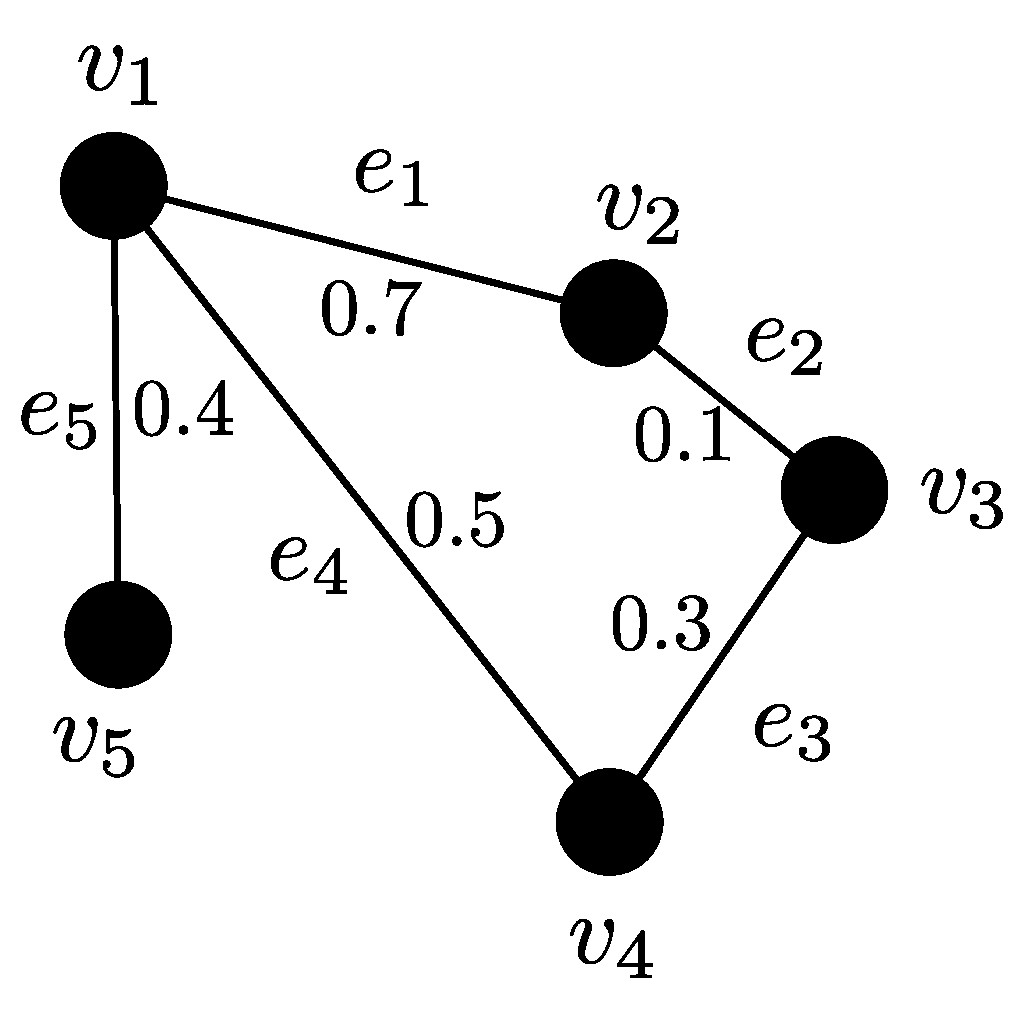
\includegraphics[width=\textwidth]{example_graph.pdf}
		\label{fig:example_graph}
	\end{subfigure}	
	\hfill
	\begin{subfigure}[t]{0.32\textwidth}
		\subcaption{}
		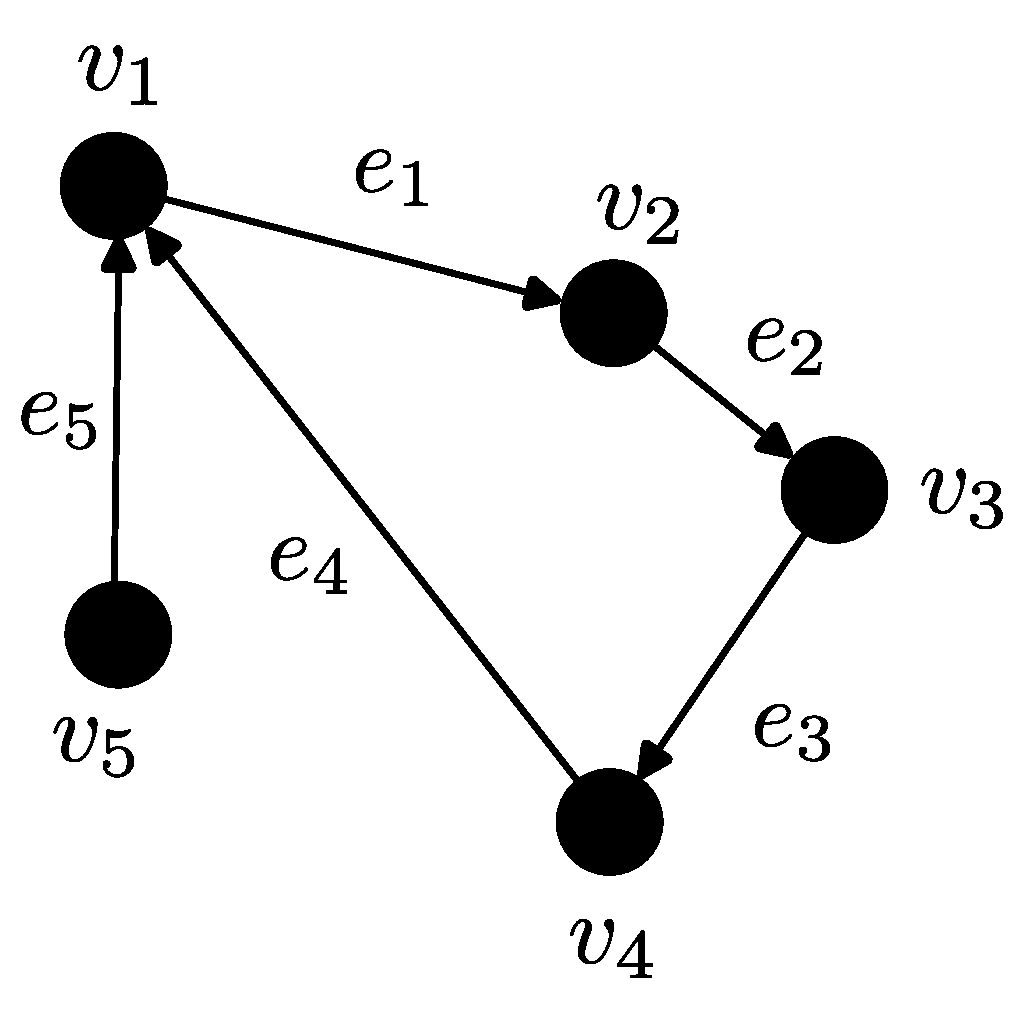
\includegraphics[width=\textwidth]{example_digraph.pdf}
		\label{fig:example_digraph}
	\end{subfigure}
	\hspace*{\fill}	
	\caption[] {\label{fig:graph_examples} \textbf{Two basic types of graphs}. (\subref{fig:example_graph}) An undirected and (\subref{fig:example_digraph}) a directed graph.}
\end{figure*}

%\begin{figure*}[!h]
%	\centering	
%	\hspace*{\fill}
%	\begin{subfigure}[t]{0.32\textwidth}
	%		\subcaption{}
	%		\includegraphics[width=\textwidth]{f6a_phantomx_hexapod.pdf}
	%		\label{fig:phantomx_robot}
	%	\end{subfigure}	
%	\hfill
%	\begin{subfigure}[t]{0.32\textwidth}
	%		\subcaption{}
	%		\includegraphics[width=\textwidth]{f6b_phantomx_pi_graph_kinematics.pdf}
	%		\label{fig:phantomx_pigraph_kin_clusters}
	%	\end{subfigure}
%	\hfill
%	\begin{subfigure}[t]{0.32\textwidth}
	%		\subcaption{}
	%		\includegraphics[width=\textwidth]{f6c_phantomx_morphology.pdf}
	%		\label{fig:phantomx_morphology}
	%	\end{subfigure}	
%	\hspace*{\fill}
%	\\
%	\hspace*{\fill}
%	\begin{subfigure}[t]{0.96\textwidth}
	%		\subcaption{}
	%		\includegraphics[width=\textwidth]{f6d_phantomx_morphology_errors_offline.pdf}
	%		\label{fig:phantomx_morphology_errors_offline}
	%	\end{subfigure}	
%	\hspace*{\fill}
%	\\
%	\hspace*{\fill}
%	\begin{subfigure}[t]{0.96\textwidth}
	%		\subcaption{}
	%		\includegraphics[width=\textwidth]{f6e_phantomx_morphology_errors_online.pdf} 		
	%		\label{fig:phantomx_morphology_errors_online}
	%	\end{subfigure}	
%	\hspace*{\fill}	
%	\caption[] {\label{fig:hexapod_simulated_results} \textbf{The hexapod robot}. (\subref{fig:phantomx_robot}) the PhantomX hexapod robot with its IMUs (red spheres), (\subref{fig:phantomx_pigraph_kin_clusters}) the kinematics graph $\mathcal{G}^{\mathcal{K}}_\pi$, (\subref{fig:phantomx_morphology}) the learned kinematic structure, errors in the estimated body structure via (\subref{fig:phantomx_morphology_errors_offline}) offline learning and (\subref{fig:phantomx_morphology_errors_online}) online learning (blue: difference rotation errors $\bar{\delta}~[\text{rad}]$, orange: sensor-to-sensor vector errors $\bar{\tilde{r}}~[\text{m}]$).}
%\end{figure*}
Two nodes $i$ and $j$ are said to be \emph{adjacent} if there is an edge $e$ connecting them. Similarly, the edge $e$ connecting the nodes is called \emph{incident} to $i$ and $j$. For example, the nodes $v_1$ and $v_4$ in Fig.~\ref{fig:example_graph} are adjacent to each other and the edge $e_4$ is incident to both nodes. The number of edges that are incident to a node is the \emph{degree} of the vertex. 

A \emph{path} represents a potential sequence of edges connecting any two given nodes. The number of edges determines the \emph{length} of the path. A graph is said to be \emph{connected} if there is at least one path between every pair of nodes; otherwise, it is labeled \emph{disconnected}. A \emph{cycle} constitutes a path comprising a minimum of three edges, where the initial and final vertices are identical, and no vertices are repeated in between. Lastly, a graph is \emph{complete} if there exists a path connecting every pair of nodes. Notice that the maximum number of edges in an undirected graph with $n$ nodes is $n(n-1)/2$

An \emph{undirected} graph lacks any specified direction assigned to its edges, meaning the connections between nodes are bidirectional. On the other hand, a \emph{directed} graph, commonly referred to as a \emph{digraph}, introduces directionality to its edges. In a directed graph, each edge has an explicit direction, indicating a one-way flow from one node to another. This directional information adds an extra layer of complexity to the relationships within the graph, as opposed to the bidirectional nature of edges in an undirected graph.

%A graph (or network) is a structure  that expresses the relationships between a set of vertices $ \mathcal{V}=\left\lbrace v_i\right\rbrace^m_{i=1}$ via a set of edges $ \mathcal{E}\subseteq \mathcal{V} \times \mathcal{V} $ with weights $ \bm{W}: \mathcal{V} \times \mathcal{V}\to \mathbb{R}_+$. Known as the weighted adjacency matrix, $ \bm{W} $ serves as the algebraic representation of $\mathcal{G}$.
A \emph{weighted} graph $ \mathcal{G}\big(\mathcal{V},\mathcal{E},\bm{W}\big) $ associates numerical value, a weight, to each edge. The weights with weights $ \bm{W}: \mathcal{V} \times \mathcal{V}\to \mathbb{R}_+$ express some quantitative measure such as distance, cost, time, or any other relevant metric depending on the context of the graph. Unlike an unweighted graph, where edges simply represent connections between nodes, a weighted graph provides additional information about the relationships between nodes. For a weighted graph, the \emph{strength} of a vertex corresponds to the sum of the edge weights associated with it.


\subsubsection{Algebraic representation of a graph}
A graph with $n$ vertices can be represented as a square $n\times n$ matrix $\bm{A}$. This algebraic representation is called the \emph{adjacency matrix} and depicts the graph's connectivity pattern; that is, the elements of the matrix indicate whether pairs of vertices $\left(i,j\right)$ are adjacent or not in the graph. Formally,
the elements of a \emph{binary} adjacency matrix $\bm{A}$ are determined as follows
% ---
\begin{equation}
	\left(\bm{A}\right)_{i,j} =
	\begin{cases}
		1 & \text{if and edge connects nodes $i$ and $j$}\\
		0 & \text{otherwise}.
	\end{cases}
\end{equation}
% --
By extension, a \emph{weighted} adjacency matrix $\bm{W}$ denotes a weighted connection for some of the $\left(i,j\right)$ entries, i.e $\left(\bm{W}\right)_{i,j} \in \mathbb{R}_+$. If the graph is undirected, the adjacency matrix is symmetric, which implies that $\bm{A}=\bm{A}^\intercal$ and $\bm{W}=\bm{W}^\intercal$respectively. Note, however, that for the case of digraphs, the adjacency matrix is not necessarily symmetric. To illustrate this, refer to the graph in Fig.~\ref{fig:example_graph}, the corresponding binary and weighted adjacency matrices are
% ---
\begin{equation*}
	\bm{A} = \begin{bmatrix}
		0 & 1 & 0 & 1 & 1\\
		1 & 0 & 1 & 0 & 0\\
		0 & 1 & 0 & 1 & 0\\
		1 & 0 & 1 & 0 & 0\\
		1 & 0 & 0 & 0 & 0\\
	\end{bmatrix}
\end{equation*} 
% ---
and
\begin{equation*}
	\bm{W} = \begin{bmatrix}
		0 & 0.7 & 0 & 0.5 & 0.4\\
		0.7 & 0 & 0.1 & 0 & 0\\
		0 & 0.1 & 0 & 0.3 & 0\\
		0.5 & 0 & 0.3 & 0 & 0\\
		0.4 & 0 & 0 & 0 & 0\\
	\end{bmatrix}.
\end{equation*} 
% ---
Similarly, for the digraph in Fig.~\ref{fig:example_digraph}, the adjacency matrix is
% ---
\begin{equation*}
	\bm{A}_D = \begin{bmatrix}
		0 & 1 & 0 & 0 & 0\\
		0 & 0 & 1 & 0 & 0\\
		0 & 0 & 0 & 1 & 0\\
		1 & 0 & 0 & 0 & 0\\
		1 & 0 & 0 & 0 & 0\\
	\end{bmatrix}.
\end{equation*} 
% ---
Notice that unless there are self loops in the graph, the main diagonal of an adjacency matrix contains only zero entries. Two other important matrices related to a graph $ \mathcal{G} $ are the degree matrix $ \bm{D}: (\bm{D}_{ii})=\sum_{j=1}^{m} w_{ij} $, a diagonal matrix whose entries are the sum of the rows of $ \bm{W} $, and the combinatorial graph Laplacian (CGL), defined as $ \bm{L}_\text{CGL} = \bm{D} - \bm{W} $ \cite{Mateos2019ConnectingdotsIdentifying}.

\paragraph*{The normalized adjacency matrix} 
The normalized adjacency matrix, defined as
% ---
\begin{equation}
	\mathbfcal{W} = \bm{D}^{-\frac{1}{2}} \bm{W} \bm{D}^{-\frac{1}{2}},
\end{equation}
% --- 
is particularly employed in spectral graph theory \cite{Spielman2012Spectralgraphtheory} and related analyses. Normalization helps account for variations in node degrees and provides a more balanced representation of the graph structure. One common application is in spectral clustering algorithms \cite{VonLuxburg2007tutorialspectralclusteringa}, where the normalized adjacency matrix is used to compute eigenvectors and eigenvalues, aiding in the identification of clusters or communities within a graph. %It also finds applications in various graph-based machine learning and data mining tasks.

\subsubsection{Subgraphs and spanning trees}
A \emph{subgraph} $\mathcal{G}_1$ is obtained by selecting a subset of the nodes of another graph $\mathcal{G}$ and a corresponding subset of the edges connecting those nodes. Formally, a graph $\mathcal{G}_1\left(\mathcal{V}_1, \mathcal{E}_1\right)$ is a subgraph of $\mathcal{G}$ if and only if $\mathcal{V}_1 \subseteq  \mathcal{V}$ and $\mathcal{E}_1 \subseteq \mathcal{E}$. This is written $\mathcal{G}_1 \subseteq \mathcal{G}$. One particular subgraph of interest in this work are spanning trees. First, a \emph{tree graph} is a graph that does not contain cycles. Such structure usually depicts a hierarchical arrangement. Consequently, a \emph{spanning tree} $\mathcal{G}_1$ of a graph $\mathcal{G}$ is a subgraph containing all the nodes in $\mathcal{G}$ and whose edges form a tree that defines paths that ensure that all the nodes remain connected. The edges of $\mathcal{G}_1$ are denoted as the branches of the tree. In general, a graph $\mathcal{G}_1$ is said to be a spanning subgraph of $\mathcal{G}$ if and only if $\mathcal{V}_1 = \mathcal{V}$ and $\mathcal{E}_1 \subseteq \mathcal{E}$. It is worth noting that every connected graph has a spanning tree and that there are $n^{n-2}$ distinct spanning trees with $n - 1$ edges on a connected graph with $n$ vertices \cite{West2001Introductiongraphtheory}. Examples of spanning trees are shown in Fig.~\ref{fig:tree_examples}.

\paragraph*{Minimum spanning tree and Kruskal's algorithm}
The minimum spanning tree of an undirected, connected, and weighted graph is the spanning tree whose edge weight sum is less than or equal to that of all other spanning trees \cite{Sefidgarminimumspanningtree}. Kruskal's algorithm \cite{Kershenbaum1972Computingminimumspanning} is the standard method to find th minimum spanning tree of a graph. In this work we use an equivalent concept, the \emph{maximum spanning tree} (MST), which corresponds to the spanning tree with maximum edge weight sum.
% ---
\begin{figure*}[!t]
	\centering	
	\hspace*{\fill}
	\begin{subfigure}[t]{0.32\textwidth}
		\subcaption{}
		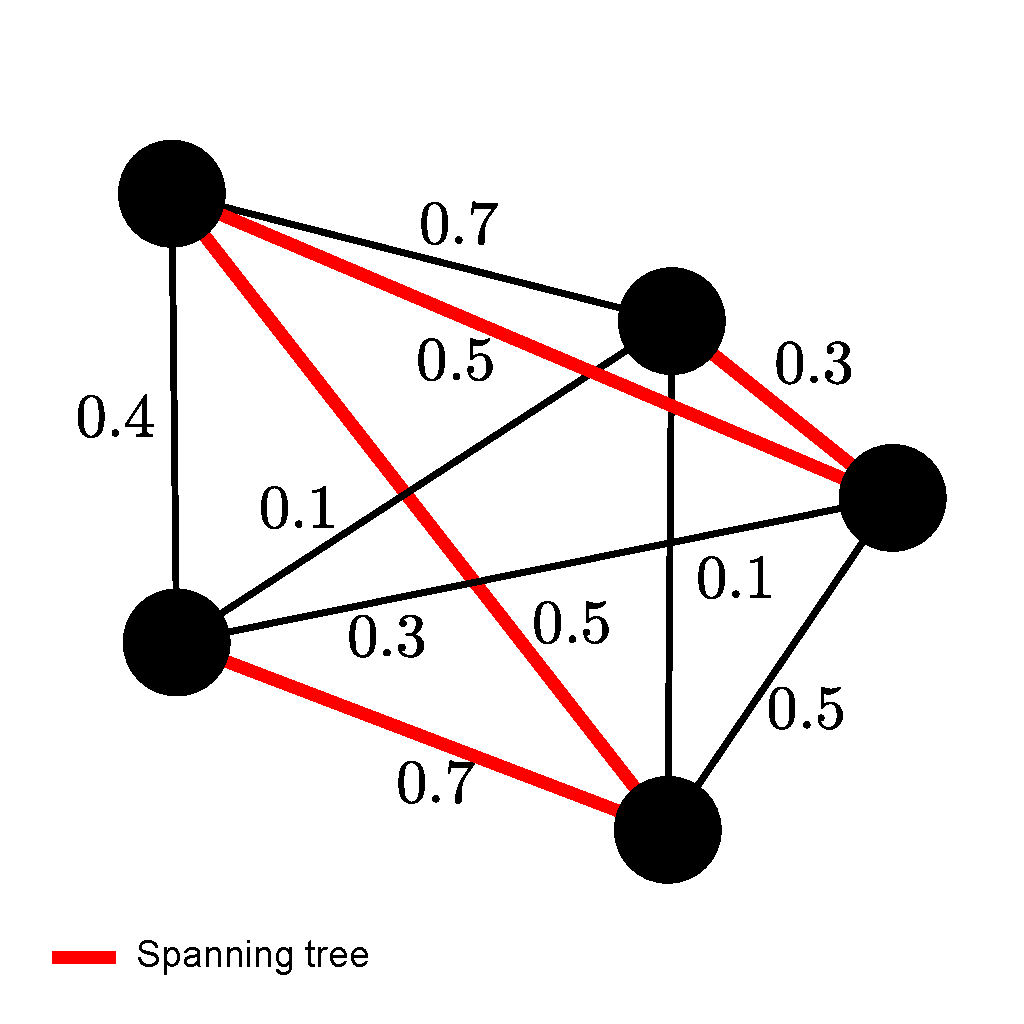
\includegraphics[width=\textwidth]{example_tree_1.pdf}
		\label{fig:example_tree_1}
	\end{subfigure}	
	\hfill
	\begin{subfigure}[t]{0.32\textwidth}
		\subcaption{}
		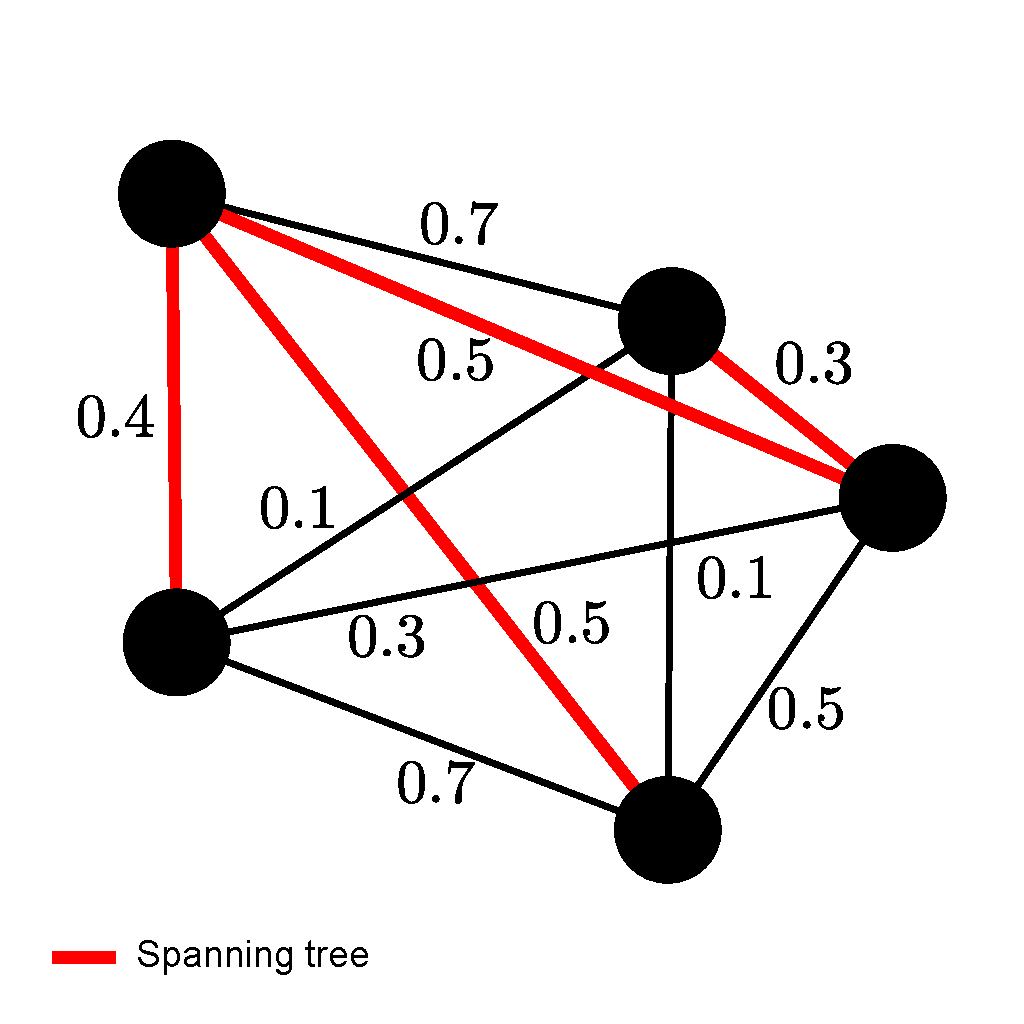
\includegraphics[width=\textwidth]{example_tree_2.pdf}
		\label{fig:example_tree_2}
	\end{subfigure}
	\hfill
	\begin{subfigure}[t]{0.32\textwidth}
		\subcaption{}
		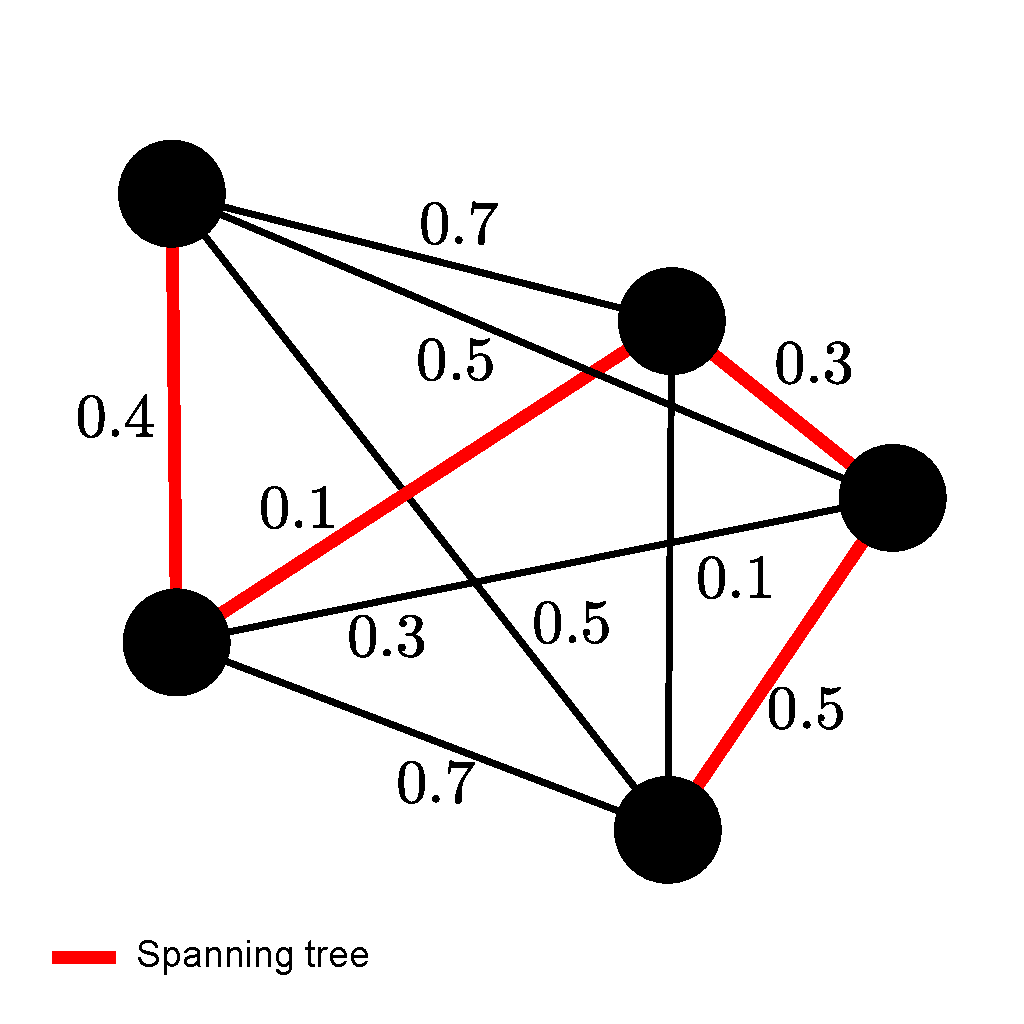
\includegraphics[width=\textwidth]{example_tree_3.pdf}
		\label{fig:example_tree_3}
	\end{subfigure}	
	\hspace*{\fill}	
	\caption[] {\label{fig:tree_examples} \textbf{Different spanning trees for the same graph}.}
\end{figure*}

% SUBSECTION ================================================================================
\subsubsection{Metrics for graph comparison}
Several works cover a number of metrics and measures to asses the similarity of any two given graphs. Commonly used metrics include eigenvalue distribution analysis \cite{Crawford2017GraphStructureSimilarity,Gera2018Identifyingnetworkstructure}, and the graph adjacency spectral and matrix distances \cite{Wills2020Metricsgraphcomparison}. This dissertation will use the latter two measures as they allow the local and global comparison of the graph structure.

\paragraph*{Spectral distance.} The spectrum of a graph $\mathcal{G}$ is the vector $ \bm{s}^{\bm{W}}$ containing the eigenvalues $s_k$ of its weighted adjacency matrix $\bm{W}$ sorted in descending order; that is
% ---
\begin{equation}
	\bm{s}^{\bm{W}} = [s_1,s_2,\ldots,s_k,\ldots,s_n]^\intercal.
\end{equation}
% ---
The spectral distance between two graphs $\bm{W}_1$ and $\bm{W}_2$ is simply the $L_2$ norm of the difference between their spectra
% ---
\begin{equation}
	d_{\bm{s}}\left(\mathcal{G}_1,\mathcal{G}_2\right) = \sqrt{\left(\bm{s}^{\bm{W}_1}-\bm{s}^{\bm{W}_2}\right)^\intercal\left(\bm{s}^{\bm{W}_1}-\bm{s}^{\bm{W}_2}\right)}.
\end{equation}
% ---

\paragraph*{Matrix distance.} This distance expresses the a direct comparison of the pairwise affinities between the graphs $\bm{W}_1$ and $\bm{W}_2$. From the many potential matrix distances, here the Frobenius distance is used; i.e,
% ---
\begin{equation}
	d_{\bm{W}}\left(\mathcal{G}_1,\mathcal{G}_2\right) =\lvert \lvert \bm{W}_1- \bm{W}_2\rvert \rvert_F.
\end{equation}
% ---

% ===========================================================================================
%                                           |                                               |
% -------------------------------------- SECTION -------------------------------------------|
%                                           |                                               |
% ===========================================================================================
\subsection{Network topology inference}\label{sec:network_topology_inference}
As mentioned before, the mechanical topology of a robot can be represented as a graph. The nodes in said graph correspond to the links and the edges indicate the joints connecting those bodies. how to obtain this graph remains unanswered. The relation between the robot morphology and information structure provides a starting point to search for the robot topology in the relationships among the sensorimotor signals. In general, the process of identifying and visually representing relationships among various elements within a system, based on the available measurements, is termed \emph{network topology inference} (NTI) \cite{Dong2019Learninggraphsdata}. Unveiling the structure of a network or graph through topology learning facilitates the analysis of interactions among entities. 

\subsubsection{Types of connectivity}
%Finding and graphically representing the relationships among the different constituent elements of a system given the available measurements is known as \emph{network topology inference} (NTI) \cite{Dong2019Learninggraphsdata}. By learning the topology of a network/graph, it is possible to reveal a structure that aids in the analysis of the interaction among the entities. As discussed in \cite{Friston2011Functionaleffectiveconnectivity}, one method to represent interaction is via \emph{functional connectivity} (FC), which is an information-theoretic
%measure that characterizes dependencies based on the probability distributions of the observed signals (examples include correlations and mutual information). FC can be further subdivided into non-directed and directed, with the latter being related to statistical causation from the data \cite{Bastos2016tutorialreviewfunctional}. In contrast, \emph{effective connectivity} refers explicitly to the dynamic (state-dependent) influence that one element on the network has on another under a particular network model of causal dynamics; i.e, it refers to coupling or directed causal influence \cite{Park2013Structuralfunctionalbrain}. Exemplary works that use the concepts above can be found in biology\cite{Zhang2017Networkbasedmachine} and neuroscience \cite{Karwowski2019Applicationgraphtheory,Sporns2018Graphtheorymethods}.

\begin{figure*}[!h]
	\centering	
	\hspace*{\fill}
	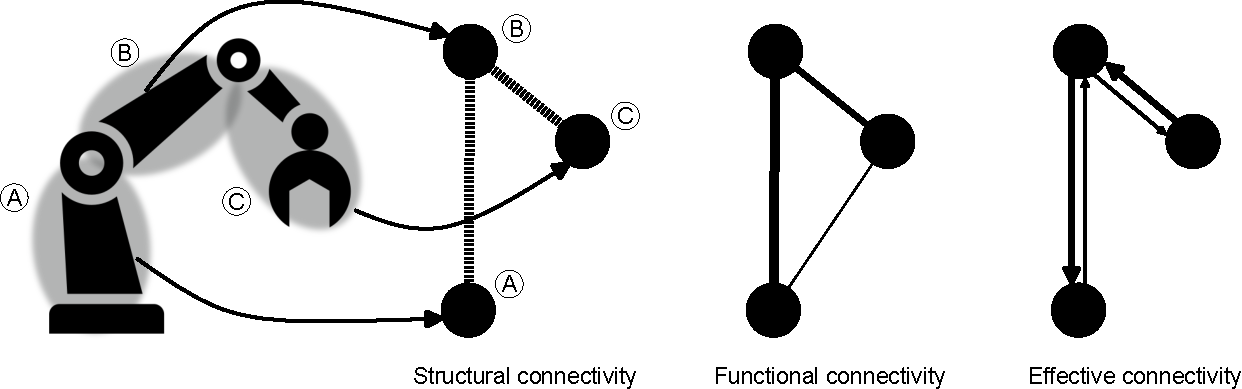
\includegraphics[width=0.9\textwidth]{types_of_connectivity.pdf}
	\hspace*{\fill}	
	\caption[] {\label{fig:types_of_connectivity}\textbf{Types of connectivity.} Every rigid body in the robot represents a node in the graphs.}
\end{figure*}

Often used in the field of neuroscience \cite{Karwowski2019Applicationgraphtheory}, three different types of connectivity are distinguished\cite{Park2013Structuralfunctionalbrain,FaskowitzEdgesbrainnetworks}:

\paragraph*{Structural Connectivity (SC)} Refers to the physical connections between different elements in a network. In the context of neuroscience, it typically involves the anatomical connections between brain regions. It is measured with techniques such as diffusion-weighted imaging (DWI) or diffusion tensor imaging (DTI) are commonly used to infer structural connectivity in the brain.

\paragraph*{Functional Connectivity (FC)} Refers to the statistical dependencies or temporal correlations between the activity of different elements in a network. As explained in \cite{Friston2011Functionaleffectiveconnectivity}, FC is an information-theoretic metric that characterizes dependencies using probability distributions of observed signals. It can be categorized into non-directed and directed forms, with the latter being associated with statistical causation derived from the data \cite{Bastos2016tutorialreviewfunctional}. %FC is often assessed through statistical methods applied to time-series data to identify patterns of correlated activity between different brain regions.

\paragraph*{Effective Connectivity (EC)} Specifically addresses the dynamic, state-dependent influence that one network element has on another within a particular causal dynamics model. Essentially, effective connectivity denotes coupling or directed causal influence \cite{Park2013Structuralfunctionalbrain}. Exemplary applications of these concepts can be observed in the fields of biology \cite{Zhang2017Networkbasedmachine} and neuroscience \cite{Karwowski2019Applicationgraphtheory,Sporns2018Graphtheorymethods}.

A representation of the intricate relationships among the three types of connectivity is given in Fig.~\ref{fig:types_of_connectivity}. It depicts a simple robot arm as an example. The nodes represent the three links that compose the robot. Regarding SC and FC, a nuanced connection exists, albeit not strictly one-to-one. For example, the SC reflect the actual physical composition of the body, three bodies connected by two joints (the edges in the SC graph). Sensory signals coming from these bodies might lead to potential functional interactions of varied degree (the edges in the FC graph) that have a foundation on the bodily structure of the robot; yet, it does not ensure their occurrence. Actually, functional relationships can appear even in the absence of direct structural connections, not the light edge between nodes $A$ and $C$ in the FC graph. Moving to EC and FC, the former extends the latter by seeking to model the direction and strength of influence between different elements. While FC identifies statistical associations, EC strives to unveil the underlying causal relationships, the directed edges in the EC graph. In summary, these three connectivity types are interrelated components in the complex landscape of NTI. Structural connections provide the anatomical substrate, functional connections depict statistical dependencies, and effective connections aspire to model causal relationships within the network.


%\redtext{The relationships between SC, FC, and EC in NTI are intricate and multifaceted. Regarding structural and functional connectivity, a nuanced connection exists, albeit not strictly one-to-one. Structural connectivity establishes the anatomical foundation for potential functional interactions, but it doesn't ensure their occurrence. Notably, functional correlations can manifest even in the absence of direct structural connections. Moving to effective connectivity and functional connectivity, the former extends the latter by seeking to model the direction and strength of influence between different elements. While functional connectivity identifies statistical associations, effective connectivity delves deeper, striving to unveil the underlying causal relationships. In summary, these connectivity types are interrelated components in the complex landscape of network topology inference. Structural connections provide the anatomical substrate, functional connections depict statistical dependencies, and effective connections aspire to model causal relationships within the network.} %While these concepts are often explored within the realm of neuroscience, their principles are versatile and applicable to understanding other intricate systems beyond the brain.
%**Relationships:**
%- **Structural and Functional Connectivity:** There is a relationship between structural and functional connectivity, but it's not one-to-one. Structural connectivity provides the anatomical substrate for potential functional interactions, but structural connections do not guarantee functional interactions, and functional correlations can occur in the absence of direct structural connections.
%
%- **Effective Connectivity and Functional Connectivity:** Effective connectivity builds upon functional connectivity by attempting to model the direction and strength of the influence between different elements. While functional connectivity identifies statistical associations, effective connectivity aims to infer the underlying causal relationships.
%
%In summary, structural, functional, and effective connectivity are interrelated aspects of network topology inference, with structural connections providing the anatomical substrate, functional connections representing statistical dependencies, and effective connections aiming to model causal relationships within the network. Techniques from neuroscience are often applied to study these aspects in the context of brain networks, but similar principles can be extended to other complex systems.

\subsubsection{Inferring the connectivity}
In NTI the elements $\mathcal{V}$ of a graph $\mathcal{G}$ are known but its connectivity (i.e. how these elements relate to each other) is unknown. %Then, the graph topology inference problem consists in finding the edges $\mathcal{E}$ that best explain the relationships among the nodes $\mathcal{V}$ given some prior knowledge, such as  data distribution, the location of the sensors, the physical relationships between the signals, or the data similarity \cite{Dong2019Learninggraphsdata,Stankovic2019Introductiongraphsignal}. 
The problem of learning the edges $\mathcal{E}$ that best explain the relationships among the $N_\mathcal{V}$ elements in $\mathcal{V}$ leads to define a graph a graph $\mathcal{G}\left(\mathcal{V},\mathcal{E},\bm{W}\right)$ with an strictly positive weighted adjacency matrix $\bm{W}$. To find this matrix, a number of sample points $m$ from the signals at the nodes $\bm{x} = [x1,x2,\ldots, x_{N_\mathcal{V}}]^\intercal \in \mathbb{R}^{N_\mathcal{V}}$ are collected into a data matrix $\bm{X} \in \mathbb{R}^{N_\mathcal{V} \times m}$. Using $\bm{X}$ together with some prior knowledge, such as  data distribution, the location of the sensors, the physical relationships between the signals, or the data similarity candidate graphs $\mathcal{G}$ can be defined \cite{Dong2019Learninggraphsdata,Stankovic2019Introductiongraphsignal}. Commonly, NTI methods are subdivided in statistical models, physically motivated models, and more recently, in methods from graph signal processing (GSP), see Fig.~. 
% ---
\begin{figure*}[!t]
	\centering	
	\hspace*{\fill}
	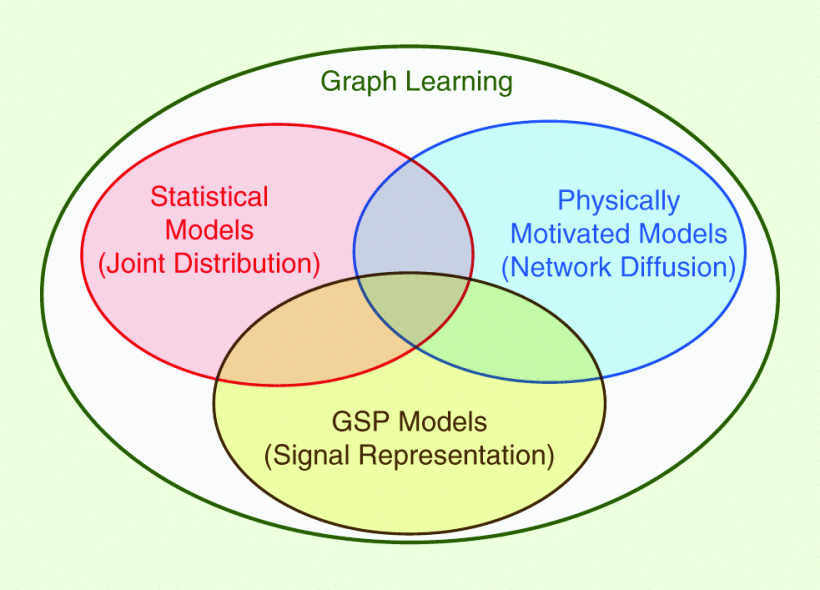
\includegraphics[width=0.5\textwidth]{graph_learning.png}
	\hspace*{\fill}	
	\caption[] {\label{fig:graph_learning}\textbf{Different methods for NTI.} Image taken from \cite{Dong2019Learninggraphsdata}.}
\end{figure*}
% ---
\paragraph*{Statistical models} These NTI methods aim to capture signal similarities, utilizing measures such as the Pearson correlation, Jaccard coefficient, Gaussian radial basis functions, and mutual information. The predominant approach involves expressing these similarities by computing the correlation of the data matrix $\bm{X}$ and assuming joint Gaussianity of the variables. The primary objective is usually to estimate the graph structure embedded in the precision matrix (defined as the inverse of the covariance matrix). However, as the precision matrix is not a proper adjacency matrix, methods have been developed to ensure Laplacian constraints (to find a valid graph) and structural constraints (to promote sparsity). Notable examples include the graphical LASSO \cite{Mazumder2011GraphicalLassoNew} and the work in \cite{Olsson2006unknownsensorsactuators,Egilmez2021GraphLaplacianLearning}. Information theory is pivotal in NTI, providing a robust framework for deducing network structures through fundamental concepts like mutual information. Numerous methodologies rooted in information theory have been proposed for network inference \cite{Lungarella2006Mappinginformationflow,Villaverde2014MIDERnetworkinference,Ursino2020TransferEntropyas,Novelli2020Inferringnetworkproperties}.%, with a particular emphasis on domains such as systems biology, bioinformatics, and various scientific disciplines.

%\paragraph*{Learning graphs from smooth signals}

\paragraph*{Psychically motivated models} Here the structure of $\mathcal{G}$ is assumed to be tied to an underlying physical phenomenon or process on the graph; for example, network diffusion processes or information propagation models.

\paragraph*{Graph signal processing} In GSP the the vector of node signals $\bm{x}$ af any given time is deemed a graph signal and is hypothesized to be a function of some process that depends on the graph; i.e., $\bm{X} = f(\mathcal{G})$. In GSP, each of the vectors $\bm{x}$ is considered a signal defined on the nodes of the weighted graph $\mathcal{G}$. Learning this graph implies determining an adjacency $\bm{W}$ such that $f(\mathcal{G})$ reflects some features in the data matrix $\bm{X}$. Examples involve learning graphs from observations of smooth signals and identifying the structure of network diffusion processes.

Of particular interest to this dissertation are the statistical methods based on information theoretic measures to determine the functional connectivity among the robot sensorimotor signals. The belief is that the FC found through these methods should be in agreement with the embodiment and information structure hypothesis and, thus, should lead to the discovery of the robot mechanical topology (which is analogous to the structural connectivity).


%With \textbf{GSP} \cite{Dong2019Learninggraphsdata}. We consider a method \cite{Kalofolias2016Howlearngraph} which learns a relational matrix $ \bm{W}_{GSP} $ without prior structural information considering the signals in $\bm{x}(t) $ as graph signals\cite{Dong2019Learninggraphsdata}. $ \bm{W}_{GSP} $ is derived under the assumption that the signals on the graph change smoothly between connected nodes. Likewise, the Graph Signal Processing Toolbox (GSPBOX) from \cite{Perraudin2014GSPBOXtoolboxsignal} was used to compute $ \bm{W}_{GSP} $ using $\alpha = 0.6$, $\beta  = 1$ (parameters that control the edge weight magnitude and the sparsity of $ \bm{W}_{GSP} $, respectively) and normalizing the required pairwise distance matrix $\bm{Z}$ between $[0,1]$.
%
%With \textbf{correlation}. The first technique \cite{Olsson2006unknownsensorsactuators} upgrades standard correlation-based NTI by searching for an inverse covariance matrix with Laplacian (to find valid adjacency matrices $ \bm{W}_{cor} $) and structural constraints (requiring a sparse matrix to reduce the graph edge density). We used the Graph Laplacian Learning (GLL) package \cite{Egilmez2021GraphLaplacianLearning} to calculate $ \bm{W}_{cor} $, with regularization parameter $\gamma = 0.07$ and using a matrix $\bm{W}_0$ as connectivity prior with zero diagonal elements and ones elsewhere (denoting lack of structural knowledge).





 % ===========================================================================================
%                                           |                                               |
% -------------------------------------- SECTION -------------------------------------------|
%                                           |                                               |
% ===========================================================================================
\subsection{Basics of information theory}
%To recapitulate, in building a body schema, an understanding of the body topology is necessary. According to the types of connectivity described in Sec.~\ref{sec:network_topology_inference}, a graph expressing the arrangement of the robot's joints and links would be equivalent to a description of its structural connectivity. But since only knowledge of the number and modalities of the sensorimotor signals is available, this SC must be extracted from the potential relationships between these signals.
%In Sec.~\ref{sec:embodiment_and_information} it was mentioned that the robot morphology influences the information structure of the sensorimotor signals. As such, expressing this structure as a graph corresponds to the inference of the functional connectivity among the robot signals. In particular, the FC among the sensorimotor signals can be captured by measures from information theory\cite{Cover1999Elementsinformationtheory}, as they are general, in the sense that they are not tied to a particular model, and expressive, as they can capture statistical relationships of linear and nonlinear nature. 
Recapitulating, the construction of a body schema necessitates an understanding of the body's topology. As discussed in Section~\ref{sec:network_topology_inference}, a graph that represents the organization of the robot's joints and links functions as a depiction of its structural connectivity. However, given the available information, restricted to the number and modalities of the sensorimotor signals, the deduction of this structural connectivity must occur from the potential relationships among these signals.

In Section~\ref{sec:embodiment_and_information}, the emphasis was on the fact that the robot's morphology shapes the information structure of sensorimotor signals. Consequently, representing this structure as a graph corresponds to the inference of the functional connectivity among the robot signals. Specifically, FC among sensorimotor signals can be captured using measures from information theory\cite{Cover1999Elementsinformationtheory}. These measures are general, as they are not tied to a specific model, and expressive, enabling the capture of statistical relationships of both linear and nonlinear nature.

\subsubsection{Entropy of random variables}

The entropy of a random variable is a function which attempts to characterize
the average uncertainty or unpredictability of a random variable. It is often used to quantify the amount of information in a random process. Formally, the entropy of a variable $X$ is a function of its probability distribution and is defined as 
% ---
\begin{equation}\label{eq:entropy}
	H(X) = -\sum_{i=1}^{n}p(x_i)\text{log}_2\left(p\left(x_i\right)\right).
\end{equation}
% ---
Similarly, the joint entropy between two random variables $ X $ and $ Y $ is dependent on the joint probability of the two variables; i.e,
% ---
\begin{equation}\label{eq:joint_entropy}
	H(X,Y) = -\sum_{i=1}^{n}\sum_{j=1}^{n} p(x_i,y_j)\text{log}_2\big(p\left(x_i,y_j\right)\big).
\end{equation}
% ---
In loose terms, entropy can be associated with the amount of information that a random variable coveys. This is exemplified in Fig.~\ref{fig:entropy_of_distributions}, where three probability distributions are displayed. Essentially. the less uniform the corresponding probability distribution, the less entropy it has, and hence the more information it provides; i.e. larger entropy value. 
% ---
\begin{figure*}[!t]
	\centering	
	\hspace*{\fill}
	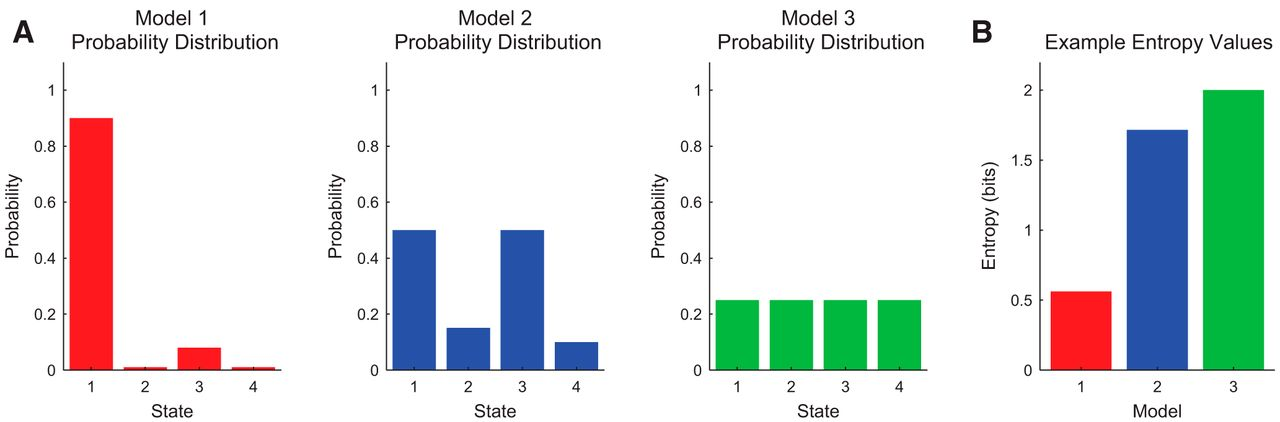
\includegraphics[width=0.9\textwidth]{entropy_of_distributions.jpg}
	\hspace*{\fill}	
	\caption[] {\label{fig:entropy_of_distributions}\textbf{Entropy of three example distributions.} The closer the distributions resemble a uniform distribution, the more information they contain. Image taken from \cite{Timme2018tutorialinformationtheory}.}
\end{figure*}
% ---

\subsubsection{Mutual Information}
The mutual information (MI) measures the amount of information that one random variable provides about another random variable. Conversely, it quantifies the reduction in uncertainty about one variable due to knowledge of the other. The MI between two random variables is a symmetric measure of information computed as the relative entropy (also known as Kullback-Leibler divergence) of the joint probability distribution $p\left(x,y\right)$ and the product of the marginal probability distributions $p\left(x\right)$ and $p\left(y\right)$; that is,
% ---
\begin{equation}\label{eq:mutual_information}
	I\left(X;Y\right) = \sum_{x \in \mathcal{X}}\sum_{y \in \mathcal{Y}}p\left(x,y\right) \text{log}_2\frac{p\left(x,y\right)}{p\left(x\right)p\left(y\right)}.
\end{equation}
% ---
Basically, this expression is comparing how similar is the joint distribution to the product of the marginals. If they are the same, $X$ and $Y$ are independent and there is no information that one can tell about the other; in other words, the MI between them is zero. Alternatively, the MI can be expressed in terms of the entropy and joint entropy as follows
% ---
\begin{equation}\label{eq:mutual_information}
	I\left(X;Y\right) =I\left(Y;X\right) = H(X) + H(Y) - H(X,Y),
\end{equation}
% ---
where it is clear why the MI is symmetric; it represents the information shared by the two random variables, see Fig.~\ref{fig:entropy_and_mutual_information}.
% ---
\begin{figure*}[!t]
	\centering	
	\hspace*{\fill}
	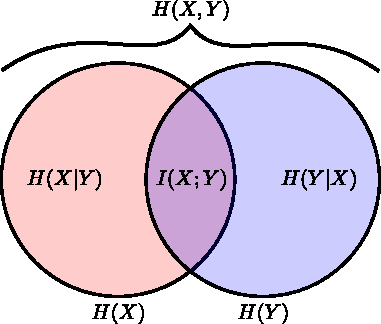
\includegraphics[width=0.5\textwidth]{entropy_and_mutual_information.pdf}
	\hspace*{\fill}	
	\caption[] {\label{fig:entropy_and_mutual_information}\textbf{Relation between entropy and mutual information.} The mutual information between two variables expresses the amount of information that one variable contains about the to other.}
\end{figure*}
% ---
\paragraph*{Connection to correlation} It is worth dedicating some time to discuss using mutual information against the well-known correlation. Both have the common objective of evaluating the interdependence between random variables. Correlation measures the intensity and directionality of a linear association between two variables, whereas MI can identify any statistical dependency---including non-linear associations. Therefore, MI represents a more comprehensive measure of the connection between variables compared to correlation, rendering it a valuable instrument to express the relations between sensorimotor variables.

\subsection{Summary}
The mechanical arrangement of the robot's joints and links referred to as topology, constitutes a crucial element of the robot body schema, playing a fundamental role in fully characterizing its kinematic and dynamic properties. As illustrated in Fig.~\ref{fig:topology_inference_process}, a robotic agent's autonomous acquisition of body topology necessitates reliance on the information structure embedded in its sensorimotor signals. The unveiling of this structure entails thoroughly examining the relationships among the sensorimotor signals using information theory measures. Once these measures are established, they can be utilized to infer the functional connectivity among the signals. In the subsequent chapter, we delve into the final step, wherein graph theory tools and first-order kinematic principles are employed to ascertain the mechanical structural connectivity based on sensorimotor functional connectivity.


% ---
\begin{figure*}[!t]
	\centering	
	\hspace*{\fill}
	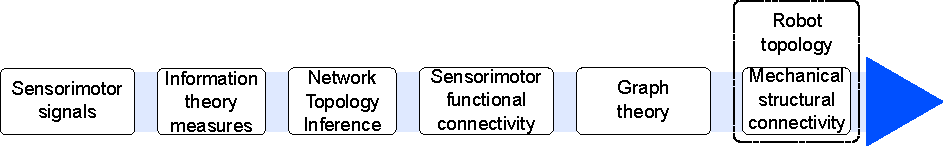
\includegraphics[width=0.9\textwidth]{topology_inference_process.pdf}
	\hspace*{\fill}	
	\caption[] {\label{fig:topology_inference_process}\textbf{Topology inference process.} Extracting the robot's mechanical topology from the relationships among the sensorimotor signals involves combining tools from information and graph theory to determine the functional connectivity between signals and using it to infer the mechanical structural connectivity.}
\end{figure*}
% ---


%% ---
%\begin{figure*}[t!]
%	\begin{center}
%		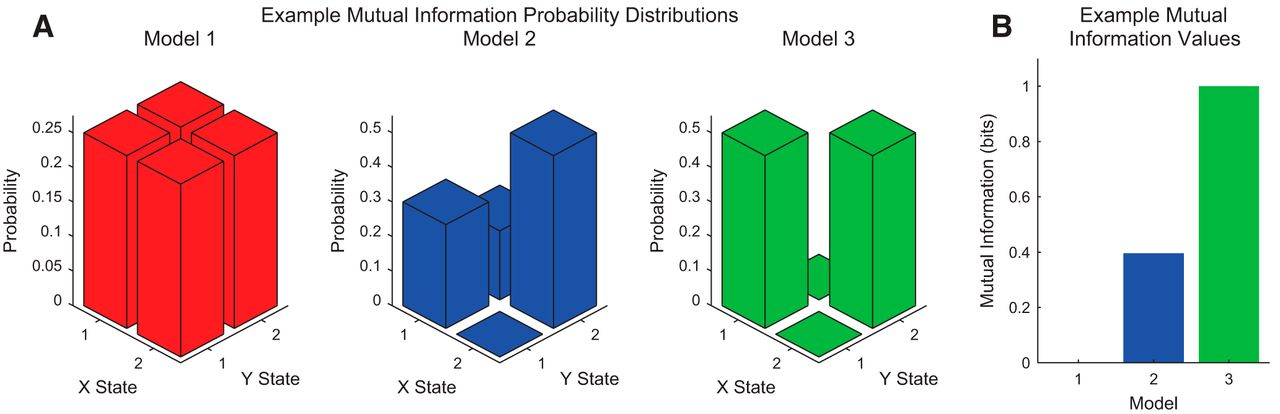
\includegraphics[width=0.9\textwidth]{mutinf_of_distributions.jpg}
%	\end{center}
%	\caption{\textbf{Mutual information of various joint distributions.} .Image taken from \cite{Timme2018tutorialinformationtheory}}
%\end{figure*}
%% ---
%As mentioned in the main text, the MI is used to create the relational matrix $\hat{\bm{W}}_{MI}$. In practice, the computation of $(\hat{\bm{W}}_{MI})_{i,j}$ involves selecting a pair $\left({x}_i(t),{x}_j(t)\right)$ of time series from the data matrix $\bm{X}$, centering their samples (to zero mean and unit standard deviation) and using either binning, kernel, or nearest neighbor methods \cite{WaltersWilliams2009Estimationmutualinformation} to compute their mutual information. Yet, such a process can be memory- and computation-demanding when the length $n$ of each of the time series is large or when streaming signals are considered. Therefore, to enable the online computation of the $m\left(m-1\right)/2$ pairwise MI values, every $N_{\mathbfcal{X}}$ points, we extract a mini-batch $\mathbfcal{X}$ from the replay buffer $\mathbfcal{B}$ and compute its corresponding MI matrix $\bm{W}^\mathbfcal{X}_{MI}$. Then, the overall MI matrix estimate $\hat{\bm{W}}_{MI}$ for the time series is the cumulative average over the previously computed matrices $\bm{W}^\mathbfcal{X}_{MI}$. To monitor its convergence, we observe the total information content in the matrix, defined as
%% ---
%\begin{equation}\label{eq:total_information}
%	T_{MI} =  \frac{1}{2}\text{tr}\left(\hat{\bm{D}}_{MI}\right),
%\end{equation}
%% ---	
%where $\hat{\bm{D}}_{MI}$ is the associated degree matrix. After the change in $T_{MI}$ falls below a threshold value $\epsilon$, namely 
%$\Delta T_{MI}<\epsilon$, $\hat{\bm{W}}_{MI}$ exhibits minimal changes in its structure. In Sec.~\nameref{sec:topology_convergence}, we provide examples of the convergence of this term for the robot manipulator, hexapod, and humanoid cases.
%
%In this work, for the computation of $\hat{\bm{W}}_{MI}  $ either offline from $\bm{X}$ or incrementally from the mini-batch matrices $\bm{W}^\mathcal{X}_{MI}$, we use the Java Information Dynamics Toolbox (JIDT) \cite{Lizier2014JIDTinformationtheoretic} and choose a kernel method to compute the MI from the signals $ \bm{x}(t) $ with a kernel width of $k = 0.8$. We alternatively used the Python machine learning library scikit-learn\cite{Pedregosa2011ScikitlearnMachine} and the open-source MATLAB package Mutual Information Computation \cite{PengMutualInformationcomputation} for comparison.

%\subsubsection{Unexplored alternatives}
%The transfer entropy \cite{Bossomaier2016introductiontransferentropy} is
%
%
%\subsection{Applications}

%Previous works have discussed metrics based on information entropy in the context of sensorimotor coordination \cite{Bonsignorio2020EntropyBasedMetrics}
% ===========================================================================================
%                                           |                                               |
% -------------------------------------- SECTION -------------------------------------------|
%                                           |                                               |
% ===========================================================================================
%\section{Differential geometry}
%
%
%\begin{figure*}[!h]
%	\centering	
%	\hspace*{\fill}
%	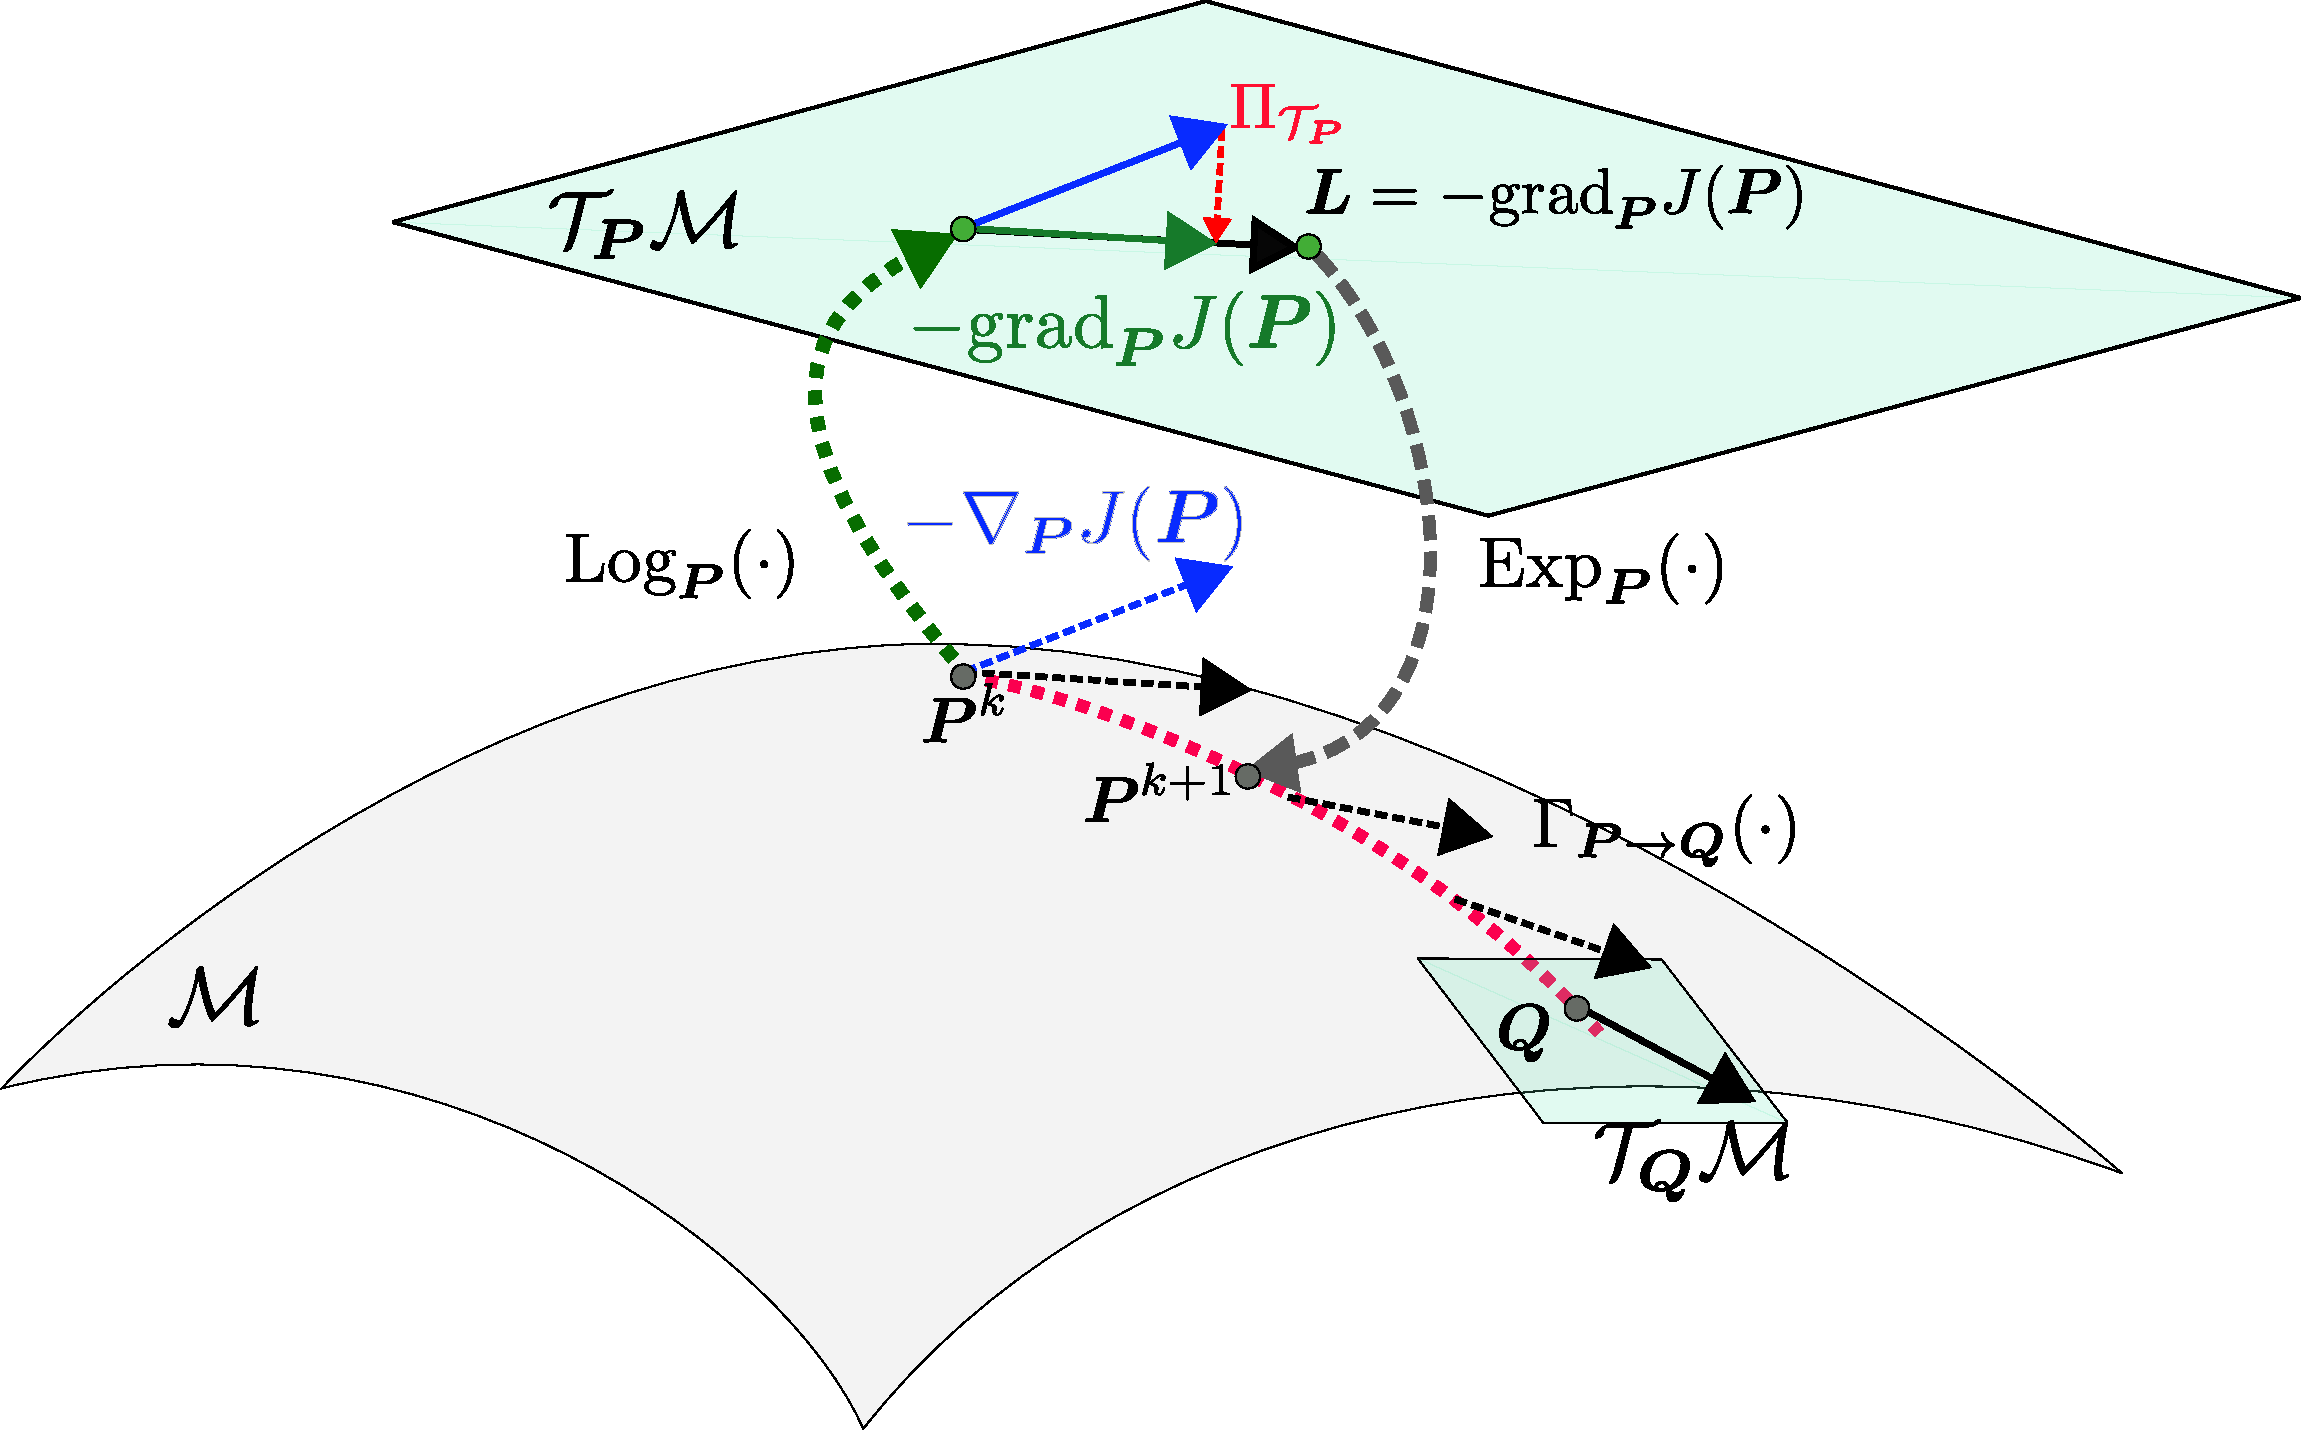
\includegraphics[width=0.5\textwidth]{manifold_operators.pdf}
%	\hspace*{\fill}	
%	\caption[] {\label{fig:manifold_operators}\textbf{Operations on a manifold.} The figure illustrates the curved space of the manifold and its associated tangent space. The logarithmic and exponential maps enable to project a point from the tangent space to the manifold space and vice-versa.}
%\end{figure*}
%
%% SUBSECTION ========================================================================================
%\subsection{The space of symmetric positive definite matrices}\label{sec:spd_manifold}
%%A \emph{differentiable manifold} $\mathcal{M}$ is a topological space that is locally similar to Euclidean space and has a globally defined differential structure \cite{Jayasumana2013KernelmethodsRiemannian}. $\mathcal{T}_{\bm{P}}\mathcal{M}$ is the \emph{tangent space} at a point $\bm{P}\in \mathcal{M}$ and represents the vector space of all the possible tangent vectors to the manifold that pass through $\bm{P}$. The pair $(\mathcal{M},\rho)$ defines a \emph{Riemannian manifold} if $ \mathcal{M} $ is differentiable and is equipped with a positive definite metric tensor $\rho$ at each point \cite{Pennec2006Riemannianframeworktensor}. 
%A differentiable manifold, denoted as $\mathcal{M}$, is a topological space that exhibits local similarity to Euclidean space and possesses a globally defined differential structure \cite{Jayasumana2013KernelmethodsRiemannian}. The tangent space at a point $\bm{P}$ in $\mathcal{M}$, denoted as $\mathcal{T}_{\bm{P}}\mathcal{M}$, encompasses the vector space containing all possible tangent vectors to the manifold that pass through $\bm{P}$. A Riemannian manifold is defined by the pair $(\mathcal{M},\rho)$, where $\mathcal{M}$ is a differentiable manifold and each point in $\mathcal{M}$ is equipped with a positive definite metric tensor $\rho$ \cite{Pennec2006Riemannianframeworktensor}.
%
%%Denoting $\mathcal{S}^n \triangleq\left\lbrace \bm{S} \in \mathbb{R}^{n \times n} : \bm{S} = \bm{S}^T\right\rbrace$ as the space of real square symmetric matrices of dimension $n \times n$. Then, the space of $n \times n$ SPD matrices $ \mathcal{S}^n_{++}\triangleq \left\lbrace \bm{P}\in \mathcal{S}^n : \bm{P} \succ 0 \right\rbrace $  defines a smooth submanifold $\mathcal{M}$ of $\mathcal{S}^n$. By definition, its tangent space $\mathcal{T}\mathcal{M} \in \mathcal{S}^n$ is equipped with an \emph{affine invariant Riemannian metric} $\rho$ \cite{Lee2018geometricalgorithmrobust}. Consequently, $ \mathcal{S}^n_{++} $ defines a Riemannian manifold. Finally, the product manifold $ \mathcal{M}^N $ of SPD manifolds is the Cartesian product $\mathcal{M}^N =\mathcal{M}_1\times \mathcal{M}_2\times \ldots \times \mathcal{M}_N$. It is the set of matrices  $\left\lbrace \left(\bm{P}_1,\ldots,\bm{P}_N\right):\bm{P}_i\in\mathcal{M}_i,\quad i=1,\ldots,N\right\rbrace$ and is also a Riemannian manifold with the metric $ \bm{\rho} =\text{diag}\left( \rho_{1},\ldots, \rho_{N} \right) $. %Similarly, the generalizations of the operators mentioned above to $\mathcal{M}^N$ are the concatenations of the individual operators for each $\mathcal{M}_i$.
%
%Let $\mathcal{S}^n$ be the space of real square symmetric matrices with dimension $n \times n$, denoted as $\mathcal{S}^n \triangleq\left\lbrace \bm{S} \in \mathbb{R}^{n \times n} : \bm{S} = \bm{S}^T\right\rbrace$. The space of $n \times n$ SPD matrices, $\mathcal{S}^n_{++}\triangleq \left\lbrace \bm{P}\in \mathcal{S}^n : \bm{P} \succ 0 \right\rbrace$, defines a smooth submanifold $\mathcal{M}$ within $\mathcal{S}^n$. Its tangent space $\mathcal{T}\mathcal{M} \in \mathcal{S}^n$ is equipped with an \emph{affine invariant Riemannian metric} $\rho$ \cite{Lee2018geometricalgorithmrobust}, thereby making $ \mathcal{S}^n_{++} $ a Riemannian manifold. Finally, the Cartesian product $\mathcal{M}^N =\mathcal{M}_1\times \mathcal{M}_2\times \ldots \times \mathcal{M}_N$ defines the product manifold of SPD manifolds.  It represents the set of matrices $\left\lbrace \left(\bm{P}_1,\ldots,\bm{P}_N\right):\bm{P}_i\in\mathcal{M}_i,\quad i=1,\ldots,N\right\rbrace$ and is also a Riemannian manifold with the metric $ \bm{\rho} =\text{diag}\left( \rho{1},\ldots, \rho{N} \right) $.
	
	
	
%	The product manifold $ \mathcal{M}^N $ of SPD manifolds is the Cartesian product $\mathcal{M}^N =\mathcal{M}_1\times \mathcal{M}_2\times \ldots \times \mathcal{M}_N$. It represents the set of matrices $\left\lbrace \left(\bm{P}_1,\ldots,\bm{P}_N\right):\bm{P}i\in\mathcal{M}i,\quad i=1,\ldots,N\right\rbrace$ and is also a Riemannian manifold with the metric $ \bm{\rho} =\text{diag}\left( \rho{1},\ldots, \rho{N} \right) $.}

%The physical feasibility constraints of the inertial parameters $\bm{\theta}_i$ of the $i$-th link, summarized in Eq.~\eqref{eq:feasibility_constraints}, are satisfied if the pseudo inertia matrix 
%%---
%\begin{equation}\label{eq:pseudo_inertia_matrix}
%	\bm{P}_i(\bm{\theta}_i)=f(\bm{\theta}_i)=\begin{bmatrix}
%		\bm{\Sigma}_i && \bm{h} \\ \bm{h}^T && m
%	\end{bmatrix} \in \mathbb{R}^{4 \times 4},
%\end{equation}
%%---
%defined for each rigid body is symmetric positive-definite \cite{Wensing2017Linearmatrixinequalities}; that is, $\bm{P}_i(\bm{\theta}_i)\in \mathcal{S}_{++}^4$. Here $ \bm{\Sigma}_i = \frac{1}{2}\text{tr}(\bm{I}_i)\mathbb{1} - \bm{I}_i\in \mathcal{S}^3 $ is called the \emph{density weighted covariance matrix}. Conversely,  $ \bm{I}_i = \text{tr}\left(\bm{\Sigma}_i\right)\mathbb{1} - \bm{\Sigma}_i \in \mathcal{S}^3_{++} $, where $\mathbb{1}$ is the $3 \times 3$ identity matrix. The requirement that $\bm{P}_i(\bm{\theta}_i) \succ 0$ implies the fully physically feasible inertial parameters are in the manifold $\mathcal{S}^4_{++}=\left\lbrace \bm{P}_i(\bm{\theta}_i) \in \mathcal{S}^{4}: \bm{P}_i(\bm{\theta}_i) \succ 0 \right\rbrace$. As explained in \cite{Lee2018geometricalgorithmrobust}, for every rigid body $i$ in the kinematic chain, there exist a pseudo inertia matrix \eqref{eq:pseudo_inertia_matrix}. This means that the set of matrices  $\left\lbrace \bm{P}_i\right\rbrace_{i=1}^N$ resides in $\mathcal{M}^N$.

%\subsection{Fundamentals of differential geometry}
%\subsection{Manifolds and the tangent space}
%\subsection{Riemannian geometry and the metric}
%\subsection{Applications in robotics}
%
%\say{The Symmetric Positive Definite (SPD) manifold is one specific type of Riemannian manifold. It is a smooth manifold where the tangent space is endowed with a Riemannian metric [2]. The Riemannian metric allows us to define various geometric notions such as the geodesic distance.}

%% ===========================================================================================
%%                                           |                                               |
%% -------------------------------------- SECTION -------------------------------------------|
%%                                           |                                               |
%% ===========================================================================================
%\section{Model learning in robotics}
%Existing learning frameworks often focus on developing forward and inverse models using either a global or local approach to capture input-output relationships \cite{NguyenTuong2011Modellearningrobot}.
%
%Global methods risk overfitting and computational overload, while local methods suffer from limited generalization and hyperparameter sensitivity \cite{Thrun2002Probabilisticrobotics,Goodfellow2016DeepLearning}. Despite advancements in computational power and data availability, deep learning faces challenges due to the neglect of prior principled knowledge, making it difficult to determine dedicated neural network architectures \cite{Baker2017Designingneuralnetwork,Elsken2019Neuralarchitecturesearch}. 
%
%\subsection{End-to-end learning}
%
%\subsubsection{Classical neural networks model learning}
%Model-learning problems using neural networks (NN) mainly involves:
%\begin{enumerate}
%	\item Input/output data collection: assumed to be available
%	\item Architecture design: usually found by trial and error
%	\item Parameter optimization/learning: via well understood schemes, e.g., backpropagation and variants
%\end{enumerate}
%Designing NN for a particular problem requires experts to determine the best topology, i.e. the number of nodes and layers, connectivity, and activation functions \cite{Matteucci2006ELeaRNTEvolutionarylearning}. Furthermore, generalization is difficult as the architecture needs to balance achieving accuracy while avoiding overfitting \cite{Rocha2005Simultaneousevolutionneural,He2015Topologicaloptimisationartificial,Matteucci2006ELeaRNTEvolutionarylearning,Kwok1995Constructivefeedforwardneural,Lawrence1998Whatsizeneural,Talebi2010NeuralNetworkBased}. Therefore, if a NN is used without any model information, large amounts of training data are required to generalize to unknown data \cite{Urolagin2012Generalizationcapabilityartificial}.
%
%\subsubsection{Topology learning related works}
%Finding NN topologies is an important and challenging step \cite{Tirumala2016Evolvingdeepneural,Rocha2005Simultaneousevolutionneural,Baker2017Designingneuralnetwork}. Normally, function approximation via NN uses empirical topologies that rely on numerous parameters and do not lend themselves to interpretation. Such models provide no insight into the actual relation between the system variables. Recent works have aimed to find optimal topologies automatically. For example, evolutionary methods have been utilized to optimize the topology of Feed Forward NN (FFNN) \cite{Rocha2005Simultaneousevolutionneural,Matteucci2006ELeaRNTEvolutionarylearning} as well as  deep NN \cite{Tirumala2016Evolvingdeepneural}, by adding/deleting connections and weights. Constructive methods \cite{Kwok1995Constructivefeedforwardneural} and pruning methods \cite{Srinivas2016LearningNeuralNetwork} have also been applied to FFNN. Another method used for FFNN represents the network as a graph and reduces its degrees-of-freedom (DoF) \cite{He2015Topologicaloptimisationartificial}. Furthermore, reinforcement learning (through Q-learning) and topology learning (using variance analysis) have also been implemented to generate architectures \cite{Baker2017Designingneuralnetwork,Castillo2007Functionalnetworktopology}. Noticeably, for learning complex dynamical systems, such as articulated robot structures, results have been limited in accuracy and generalization capabilities \cite{NguyenTuong2011Modellearningrobot,NguyenTuong2008Learninginversedynamics,NguyenTuong2010Usingmodelknowledge}. 
%
%\subsubsection{Robot inverse dynamics estimation via classical NN}\label{sec:classic_inv_dyn}
%NN have been applied in numerous variants to model robot inverse dynamics. In \cite{Atencia2015Hopfieldnetworksoptimization}, Hopfield NN were applied to identify the inertial parameters. Likewise, in \cite{Zhu2014Inertiaparameteridentification} a FFNN that used the regressor matrix as training samples was applied. Extreme Learning Machines were utilized in \cite{Bargsten2016ExperimentalRobotInverse} with the same purpose. More recently a two-hidden-layers network with rectified linear activation units (ReLU) was used in \cite{Christiano2016TransferSimulationReal}. Similarly, recurrent NN have been used to account for the sequential nature of the data. In \cite{Yan1997Robotlearningcontrol}, a recurrent NN in the hidden layer of an otherwise conventional three-layer FFNN was proposed. Additionally, self-organizing-networks, in conjunction with echo state networks, were used in \cite{Polydoros2015Realtimedeep} via a real-time deep learning algorithm.
%% ===========================================================================================
%%                                           |                                               |
%% -------------------------------------- SECTION -------------------------------------------|
%%                                           |                                               |
%% ===========================================================================================
%\section{Data-driven learning with structure information}
%In lieu of the challenges faced by deep learning to capture the intricacies of complex systems from scratch,  
%Issues such as low sample efficiency, extended training times, and limited generalization highlight the necessity of balancing data-driven and principle-driven approaches \cite{Pierson2017Deeplearningrobotics,Suenderhauf2018limitspotentialsdeep}. Recently, there has been a growing acknowledgment of the importance of integrating structure into the learning of physical systems \cite{Geist2021Structuredlearningrigid,Lutter2023Combiningphysicsdeep}.
%
%% ===========================================================================================
%%                                           |                                               |
%% -------------------------------------- SECTION -------------------------------------------|
%%                                           |                                               |
%% ===========================================================================================
%\section{Model learning and the body schema}
%
%
%
%
%Building on the significance of structure in model learning for robotics, this dissertation addresses the inference of essential morphological properties in tree-like floating base structures, mimicking the development of a body schema. Efforts in cognitive robotics stress the pivotal role of internal body models in enhancing spatial awareness, motor control, and adaptability \cite{Nguyen2021Sensorimotorrepresentationlearning,Hoffmann2010Bodyschemarobotics}. However, consensus is lacking on what constitutes a robot's body schema. Some approaches focus solely on learning the kinematic structure, relying predominantly on off-body vision \cite{Hersch2008Onlinelearningbody,MartinezCantin2010Bodyschemaacquisition,Hart2011roboticmodelecological,Lipson2019Taskagnosticself,Chen2022Fullybodyvisual,Sturm2009Bodyschemalearning}. Others explore sensorimotor associations between proprioceptive, tactile, and visual modalities \cite{Fuke2007BodyImageConstructed,Malinovska2022connectionistmodelassociating,Nguyen2019Reachingdevelopmentvisuo,Pugach2019BrainInspiredCoding,Lanillos2016Yieldingselfperception}, but they provide limited insights into the robot's physical structure.
%
%Model-based robotics offers reliable methods for identifying physical attributes of robots based on known mechanical topologies. Conventional calibration routines \cite{Hollerbach1996CalibrationIndexTaxonomy} and offline system identification methods \cite{Swevers2007Dynamicmodelidentification,LeboutetInertialParameterIdentification} are effective for known kinematic structures in controlled environments. However, these methods face challenges when applied to floating base robots without standardized identification procedures \cite{Ayusawa2014Identifiabilityidentificationinertial,Lee2022OptimizedSystemIdentification}. Importantly, these conventional methods were not initially designed for integration into online learning frameworks. While model-based robotics addresses kinematic calibration and forward/inverse kinematics, it provides limited insights into the comprehensive understanding of joint and link arrangement, known as mechanical topology. In cognitive robotics, only a few studies have approached this problem for self-modeling and monitoring, relying on exteroceptive vision \cite{Bongard2006Automatedsynthesisbody,Bongard2006Resilientmachinescontinuous}. Regardless of the approach taken---black-box machine learning, cognitive methods, or model-based robotics---reliance on external measurement devices persists, overlooking embodied sensing modalities.
%
%In summary, current robotics research reveals gaps in understanding and methods for refining body models. A comprehensive interpretation of the robot body schema and the determination of essential features are crucial. Identifying the fundamental set of necessary signals, both proprioceptive and embodied exteroceptive, is paramount. Integrating advanced machine learning with prior information and first-order principles shows promise for enhanced body models, addressing data requirements and generalization issues. However, the lack of synergy between modeling and learning approaches, along with the absence of a unified scheme for relevant learning stages, represents notable gaps requiring attention to advance robotics into more sophisticated and adaptable embodied systems.
%
%\section{Model learning in robotics}
%\subsection{Classical and recent works in system identification}
%\subsection{Local and global models linear models}
%\subsection{End-to-end learning (black box models)}
%\section{Data-driven learning with structure information}
%\section{Model learning and the body schema}
%\subsection{Internal representations}
%\subsection{Sensorimotor maps}

% ===========================================================================================
%                                           |                                               |
% -------------------------------------- SECTION -------------------------------------------|
%                                           |                                               |
% ===========================================================================================
\section{Driving learning and adaption: Advanced gradient descent}

\subsection{Offline and online learning}
In the realm of machine learning, online learning and offline learning represent distinct approaches to model training. Online learning, or incremental learning, involves learning the model as new data becomes available, typically processing one observation at a time. In this scenario, the learning algorithm's parameters are updated after each individual training instance, making it particularly advantageous for systems dealing with a continuous flow of data that must rapidly adapt to changing conditions. On the other hand, offline learning, also known as batch learning, entails training the model over all observations in a dataset $\mathcal{D}$ simultaneously. The model is trained with a static dataset, and the parameters are updated once the learning process is complete for the entire dataset. %Offline learning is more prevalent in industry due to its various advantages, such as simplicity and ease of implementation. In essence, online learning is a dynamic approach where the model adapts to new data in real-time, while offline learning is a more static method where the model is trained on a fixed dataset.

%In contrast, online learning excels in real-time adaptation and efficient resource utilization, making it more appropriate for scenarios with continuously changing data patterns[4][12]. 

\subsection{Fundamentals of gradient descent}

Gradient descent (GD) is in essence an optimization algorithm to sequentially minimize a \emph{cost function} $J(\bm{x})$ with respect to a given set of parameters $\bm{x} \in \mathbb{R}^d$ moving in the direction opposite to its gradient $\nabla_{\bm{x}}J(\bm{x})$ at the current point $\bm{x}_k$. GD is considered a local optimizer as it primarily finds a local minimum of $J$. The algorithm can be summarized in a iterative process expressed in the simple equation
% ---
\begin{equation}\label{eq:gradient_descent}
	\bm{x}_{k+1} = \bm{x}_k - \eta  \nabla_{\bm{x}_k} J(\bm{x}_k;\mathcal{D}),
\end{equation}  
% ---
which gives the update $\bm{x}_{k+1}$ to the optimization variables using a \emph{learning rate} $\eta$ that controls the size of the step given in the negative direction of the gradient. If this hyperparameter is too small, the updates $\bm{x}_{k+1}$ will differ slightly from $\bm{x}_k$ and convergence will take a long time. On the contrary, if $\eta$ is too large, the parameter updates may oscillate around a local optima and even diverge. 
% ---
\begin{figure*}[t!]
	\begin{center}
		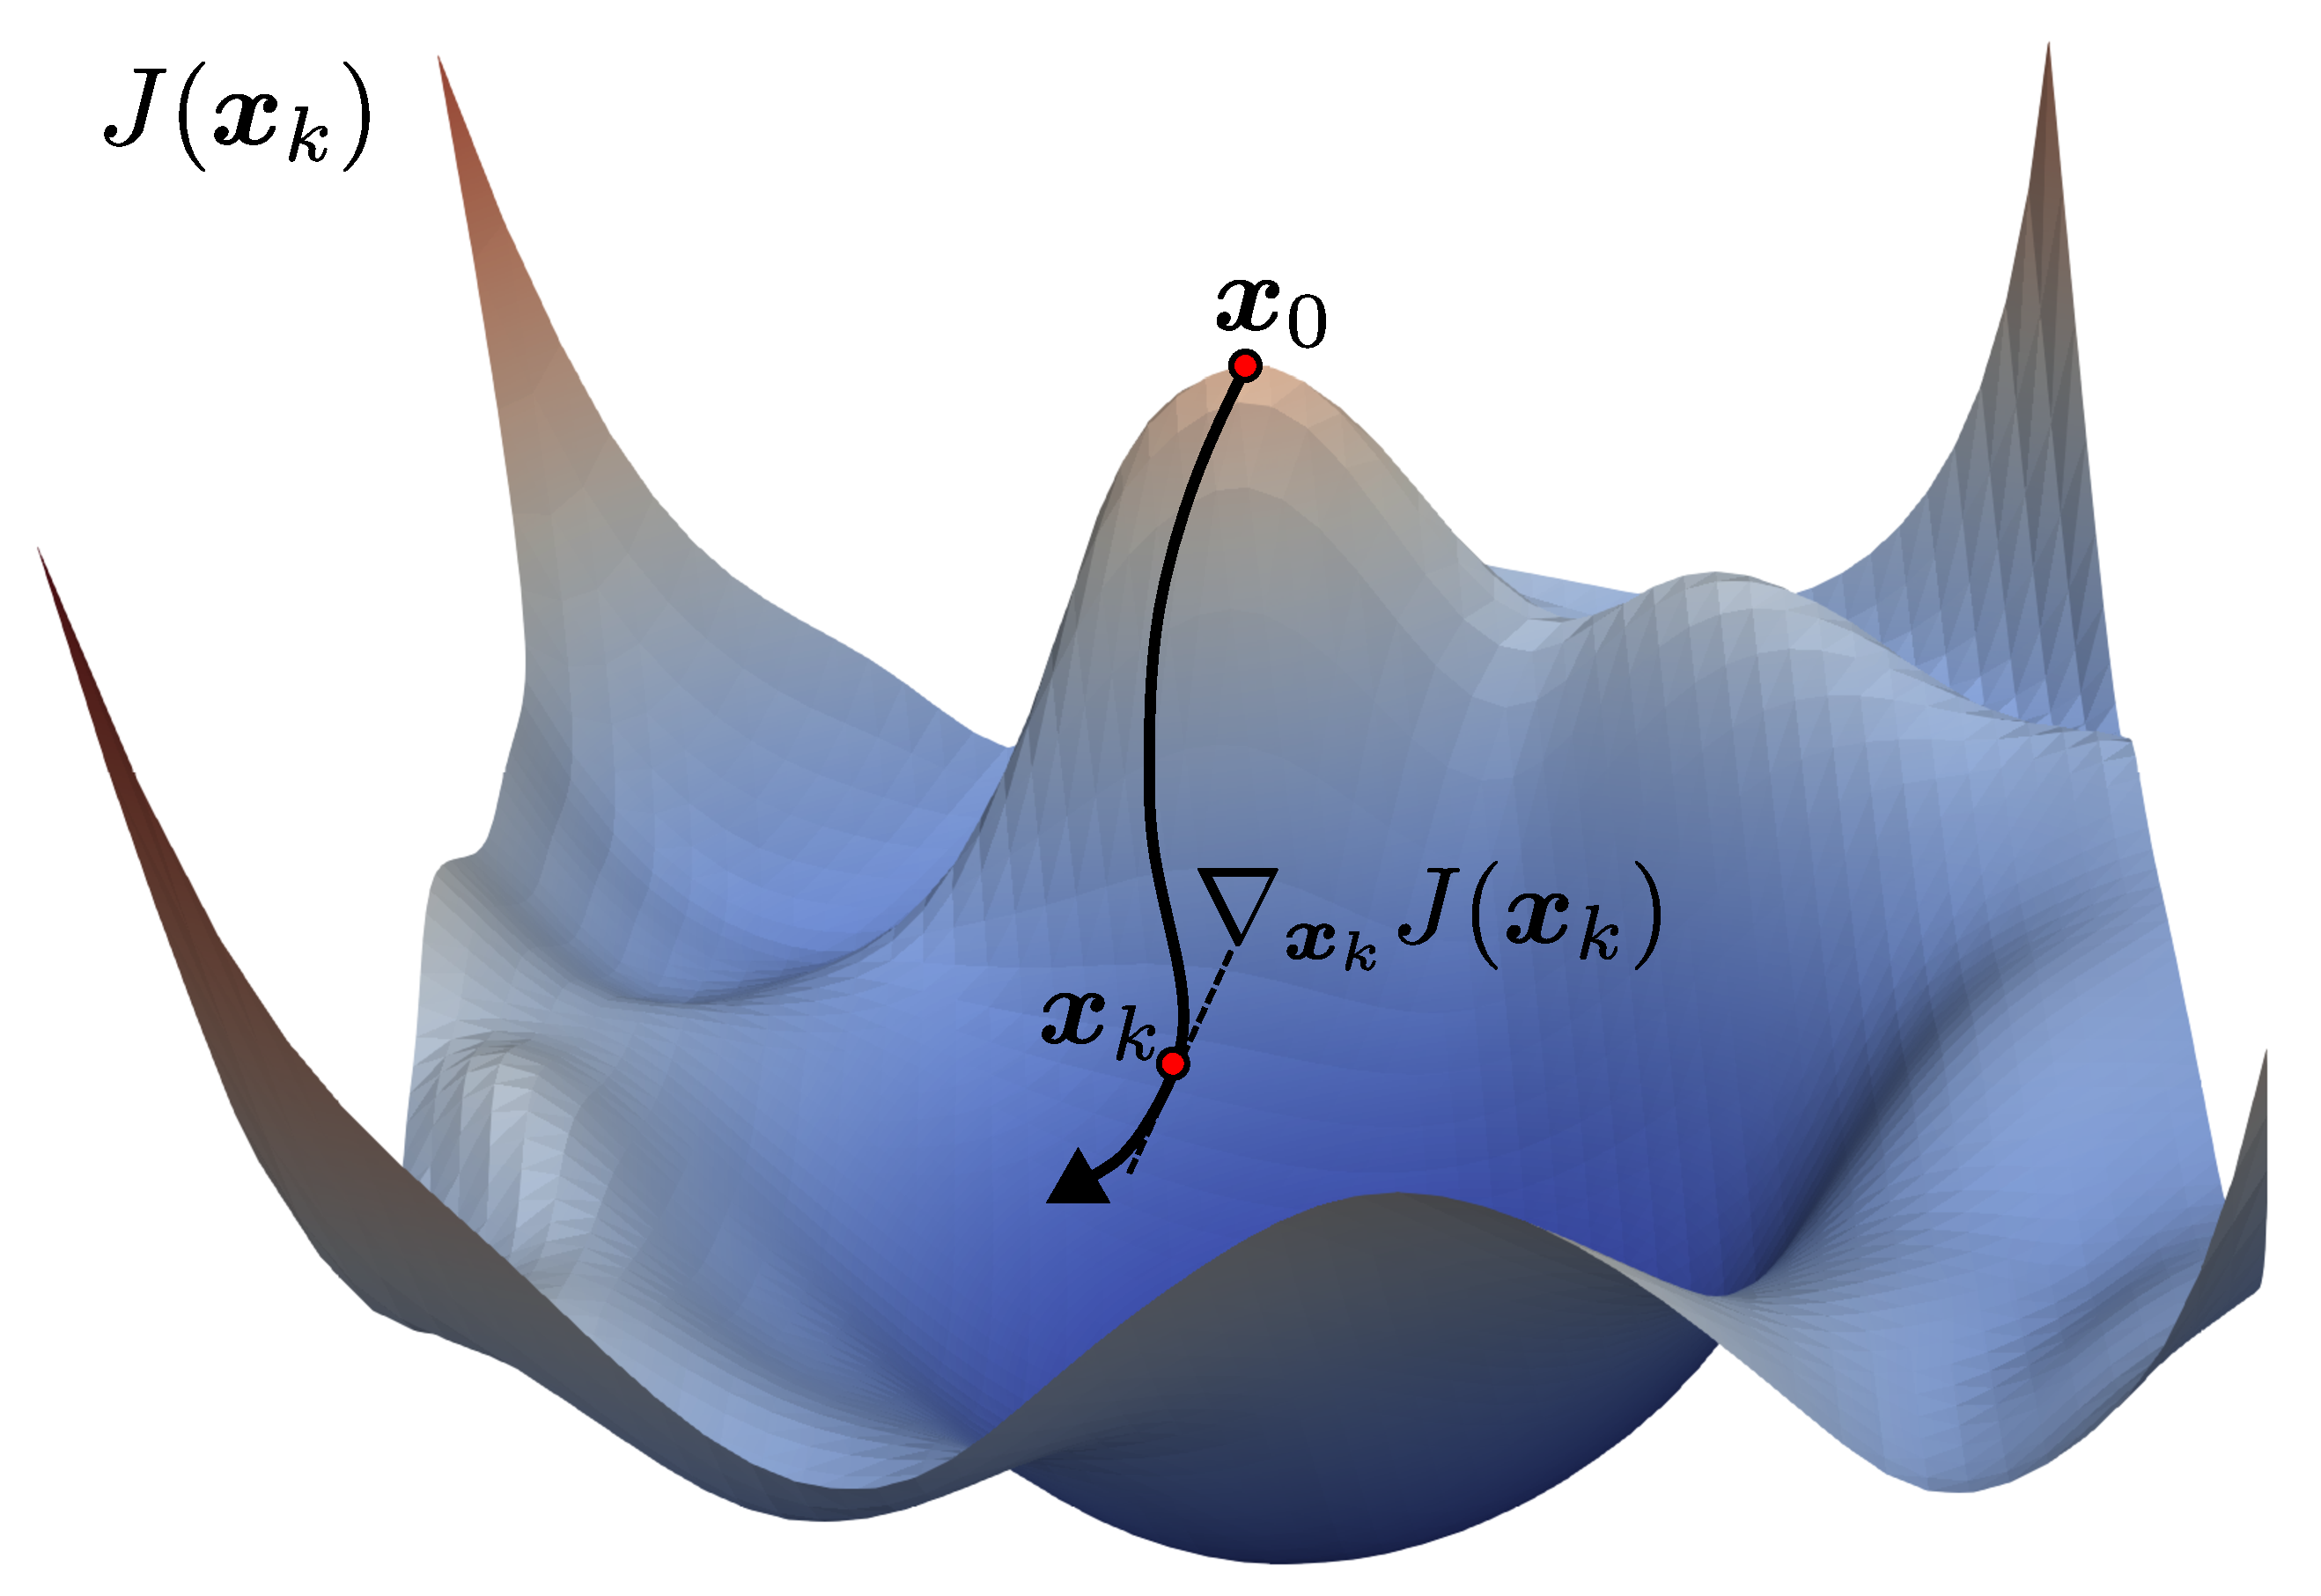
\includegraphics[width=0.5\textwidth]{gradient_descent_concept.pdf}
	\end{center}
	\caption{\textbf{Concept art gradient descent.} Image credits: \url{https://www.cs.umd.edu/~tomg/projects/landscapes/}}
\end{figure*}
% ---
From the number of data points from an already-collected dataset $\mathcal{D}$ that are used to represent the optimization cost function $J$, three variants of GD are typical: batch, stochastic, and mini-batch GD. If all data in $\mathcal{D}$ is used to compute the gradient, it is called batch GD. It relies on a static dataset and substantial computational resources (CPU, memory, and storage) for training and thus lacks the flexibility to adapt incrementally to new data. This inability to incorporate new observations in real-time hinders its applicability for online learning in dynamic environments with constantly evolving data streams. 
%The time-intensive nature of batch GD exacerbates its limitations, as updating the model with new data requires the retraining of the entire dataset, proving computationally expensive. Additionally, batch GD is less flexible in handling changing or large datasets, making it more suitable for stable scenarios with ample resources. Finally, batch learning systems lack the ability to learn incrementally, a significant drawback when dealing with streaming data or scenarios where the data distribution frequently changes.

Stochastic Gradient Descent (SGD) \cite{Bottou2012Stochasticgradientdescent} serves as a simplification of batch GD and is widely employed machine in machine learning for online learning due to its efficiency with large-scale datasets and its ability to adapt to new data one observation at a time. Its advantages lie in its speed, processing quicker parameter updates, and memory efficiency. A recent review \cite{Tian2023RecentAdvancesStochastic} discusses the the properties of SGD as a standard optimization algorithm in deep learning. Despite its ability to escape local minima, the noisy updates of SGD and bouncing behavior near the minimum can yield good but non-optimal solutions \redtext{REF}. When the gradient of the cost function is computed using a small subset or mini-batch of $\mathcal{D}$, rather than a single example or the entire dataset, SGD becomes mini-batch GD. This approach reduces the noise in the parameter updates compared to SGD, leading to more stable convergence. It allows for computational efficiency as the mini-batch can be processed in parallel, and it is typically faster than batch GD for convergence.

\subsection{Improved gradient descent}
The challenges associated with standard (commonly named vanilla) GD encompass critical issues. First, there is the already mentioned sensitivity to the selected learning rate $\eta$. Noisy gradients are a particular problem of SGD and mini-batch GD. These may lead to slower and less stable training compared to batch GD. The algorithms may also encounter obstacles like local minima and saddle points, particularly problematic in non-convex optimization problems, hindering the discovery of the global minimum.

Various improvements have been proposed to improve vanilla GD in recent years \cite{Ruder2016overviewgradientdescent,Tian2023RecentAdvancesStochastic}. Noteworthy among these enhancements are the incorporation of a momentum term, adaptive learning rate mechanisms, and measures to handle very small step sizes. The momentum term, functioning as a moving average over past gradients, serves to smooth out steps in gradient descent, thereby mitigating oscillations and expediting convergence. Its purpose is to combat issues such as bouncing around the search space and getting stuck in flat regions, ultimately elevating the optimization algorithm's efficacy and yielding superior final results.

The adaptive learning rate, tailored individually for each parameter based on the square root of the sum of the squares of historical gradients, facilitates larger updates for infrequent parameters and smaller updates for frequent ones. This adaptability proves beneficial for handling sparse data and managing sparse gradients. The approach aims to expedite convergence in the presence of sparse data by adjusting the learning rate according to the loss function's geometry. This allows for swift convergence in steep gradient directions and more cautious updates in flatter gradient directions.

However, a notable drawback of learning rate adaption is the its potential reduction to infinitesimally small values over time, limiting the ability to acquire additional knowledge. To counteract this issue, a decaying average of squared gradients was proposed to adjust the step size for each parameter. This adaptive strategy stabilizes the learning process, preventing oscillations in the optimization trajectory and proving effective for non-convex optimization problems commonly encountered in machine learning.

%
%\paragraph*{ Gradient descent with momentum.} In cost functions that change rapidly in one parameter direction and rather slowly in others, regular GD oscillates heavily in directions quasi perpendicular to the gradient and makes meager progress towards the minimum. This algorithm dampens this oscillations and accelerateseAlso known as Nesterov's accelerated gradient, Accelerates faster towards the minimum and increases the chance of escaping local minima
%\subsection{Adaptive gradient descent}
%Known commonly as AdaGrad. It adapts the updates relative to the sum of the accumulated squared gradients. This has the effect of balancing the increments given to all descent directions and results in a \say{straighter} path towards the minimum. Unfortunately, because of the gradient accumulations, updates quickly become rather small and this leads to a rather slow convergence,
%
%\subsection{RMSProp}
%Root Mean Square Propagation. It adds decay rate to the sum of past squared gradient giving important to only the recent ones.n
%
%
%\begin{center}
%	\begin{tabular}{ |c|c|c| } 
	%		\hline
	%		\textbf{Algorithm} & \textbf{Update} & \textbf{Details} \\ 
	%		\hline
	%		Momentum & cell5 & cell6 \\ 
	%		\hline
	%		NAG & cell8 & cell9 \\ 
	%		\hline
	%		Adagrad & cell8 & cell9 \\ 
	%		\hline		
	%		Adadelta & cell8 & cell9 \\ 
	%		\hline
	%		RMSProp & cell8 & cell9 \\ 
	%		\hline
	%		ADAM & cell8 & cell9 \\ 
	%		\hline
	%		AdaMax & cell8 & cell9 \\ 
	%		\hline
	%		NADAM & cell8 & cell9 \\ 
	%		\hline
	%		NADAM & cell8 & cell9 \\ 
	%\hline		
	%	\end{tabular}
%\end{center}



\subsubsection{Adaptive moment estimation: Adam}
Adaptive Moment Estimation GD, commonly known as Adam \cite{Kingma2014Adammethodstochastic}, has become a powerful optimization technique standard in machine learning. Adam is an adaptive learning algorithm that refines SGD approach by incorporating both first-order moment estimates ($m_t$) and second-order moment estimates ($v_t$) of the gradients; that is
% ---
\begin{align}\label{eq:adam_mean_and_uncentered_variance}
	\begin{split} 
		m_k &= \beta_1 m_{k-1} + \left(1 - \beta_1 \right) \nabla_{\bm{x}_k} J(\bm{x}_k;\mathcal{D}) \\ 
		v_k &= \beta_2 v_{k-1} + \left(1 - \beta_2\right) \left( \nabla_{\bm{x}_k} J(\bm{x}_k;\mathcal{D}) \right)^2 ,
	\end{split}
\end{align}
% ---
where the moving averages of the momentum term and the squared gradients  is adjusted via the discount factors $\beta_1 \in [0,1]$ and $\beta_2 \in [0,1]$. The adaptive nature of Adam stems from dynamically adjusting learning rates $\left\lbrace \eta_i\right\rbrace^d_{i=1}$ for each parameter based on the historical gradient information. This feature addresses a longstanding challenge in machine learning---manual tuning of learning rate $\eta$. The ability of Adam to autonomously adjust rates during training alleviates the need for meticulous parameter tuning, a characteristic that sets it apart from its predecessors.

A fundamental strength of Adam lies in its incorporation of momentum, which enables Adam to persist in the correct direction, surmounting obstacles such as flat regions or saddle points in the cost function $J$. Furthermore, Adam introduces a bias correction mechanism, particularly beneficial in the initial stages of training when moment estimates might be imprecise\footnote{The terms $v_k$ and $m_k$ are biased towards their zero initial value.}. This correction, computed as
% ---
\begin{align}\label{eq:adam_bias_correction}
	\begin{split} 
		\hat{m}_k &= \dfrac{m_k}{1 - \beta_1} \\ 
		\hat{v}_k &= \dfrac{v_k}{1 - \beta_2},
	\end{split} 
\end{align}
% --
enhances the accuracy of the mean and uncentered variance estimates in \eqref{eq:adam_mean_and_uncentered_variance}, contributing to the algorithm's robustness. The update rule for Adam, based on Eqs.~\eqref{eq:adam_bias_correction} and \eqref{eq:adam_mean_and_uncentered_variance}, yields
% ---
\begin{equation}
	x_{k+1} = x_{k} - \dfrac{\eta}{\sqrt{\hat{v}_t} + \epsilon} \hat{m}_t.
\end{equation}
% ---
Note that according to \cite{Kingma2014Adammethodstochastic}, the default values of $\beta_1 = 0.9$, $ \beta_2 = 0.999 $, and $\epsilon =10^{-8}$ seem to work well in practice.

Adam's computational efficiency is a standout feature, showcasing its prowess in a diverse array of applications. It has demonstrated a tendency to converge faster and demand less hyperparameter tuning than traditional SGD. Notably, Adam's adaptability to sparse or high-dimensional data renders it well-suited for complex models where different parameters may necessitate varying learning rates. This adaptability is particularly advantageous in real-world scenarios where data is inherently noisy.

The algorithm's ability to handle noisy gradients effectively speaks to its stability during training, contributing to the robustness that makes Adam a preferred choice in modern machine learning applications.% While Adam's success is undeniable, it is essential to acknowledge that the choice of optimization algorithm depends on specific problem characteristics. Variants such as RMSprop or AdaGrad may also prove effective in certain contexts, and the performance can vary based on the dataset and the model architecture.


%\paragraph*{ Gradient descent with momentum.} In cost functions that change rapidly in one parameter direction and rather slowly in others, regular GD oscillates heavily in directions quasi perpendicular to the gradient and makes meager progress towards the minimum. This algorithm dampens this oscillations and accelerateseAlso known as Nesterov's accelerated gradient, Accelerates faster towards the minimum and increases the chance of escaping local minima
%\subsection{Adaptive gradient descent}
%Known commonly as AdaGrad. It adapts the updates relative to the sum of the accumulated squared gradients. This has the effect of balancing the increments given to all descent directions and results in a \say{straighter} path towards the minimum. Unfortunately, because of the gradient accumulations, updates quickly become rather small and this leads to a rather slow convergence,
%
%\subsection{RMSProp}
%Root Mean Square Propagation. It adds decay rate to the sum of past squared gradient giving important to only the recent ones.n
%
%\subsection{ADAM gradient descent}
%Adaptive Moment Estimation. In essence a combination between the effects of momentum and RMSProp; that is, it inherits the speed from momentum and the ability to adapt the gradient directions.
\subsubsection{AMS gradient descent}


AMSGrad is a gradient descent method that aims at convergence issues faced by Adam and its variations \cite{Reddi2019convergenceadam}; which have been observed to exhibit issues related to the learning rate, where it may become too aggressive and lead to poor convergence behavior in certain scenarios. AMSGrad tries to address this issue by modifying the way it updates the parameters. 

The key improvement introduced by AMSGrad lies in its handling of the adaptive learning rates for each parameter. In the original Adam algorithm, the learning rates are adapted based on the exponential moving averages of the first-order moment (mean) and the second-order moment (uncentered variance) of the gradients. However, Adam does not incorporate a mechanism to correct the bias in the estimate of the second-order moment, which can lead to an overly aggressive decrease in the learning rates.

AMSGrad addresses this limitation by modifying the update rule for the moving average of the second-order moment. Unlike Adam, AMSGrad maintains a running average of the past squared gradients for each parameter without bias correction. Particularly, instead of using $\hat{v}_t$ as in \eqref{eq:adam_bias_correction}, its previous value $\hat{v}_{k-1}$ is used as long as it is greater than the current value computed according to \eqref{eq:adam_mean_and_uncentered_variance}; i.e.,
% ---
\begin{equation}
	\hat{v}_t = \text{max}(\hat{v}_{t-1}, v_t).
\end{equation}
% ---
The update rule for AMSGrad 
% ---
\begin{equation}
	x_{k+1} = x_{k} - \dfrac{\eta}{\sqrt{\hat{v}_t} + \epsilon} m_t
\end{equation}
% ---
excludes also the regularization of the first momentum term. The alteration to the second moment ensures that the denominator in the learning rate calculation does not become excessively small over time, preventing the learning rate from growing uncontrollably small.

In essence, AMSGrad aims to provide a more stable and consistent learning rate, preventing scenarios where the learning rate diminishes rapidly and adversely affects convergence. By addressing this issue, AMSGrad aims to offer improved convergence behavior and generalization, particularly in cases where Adam might exhibit erratic behavior due to the uncorrected bias in the second-order moment estimate.

%\subsubsection{Riemannian gradient descent on $ \mathcal{S}^{4}_{++} $}
\subsubsection{Gradient descent on Riemannian manifolds}
% ---
\begin{figure*}[!t]
	\centering	
	\hspace*{\fill}
	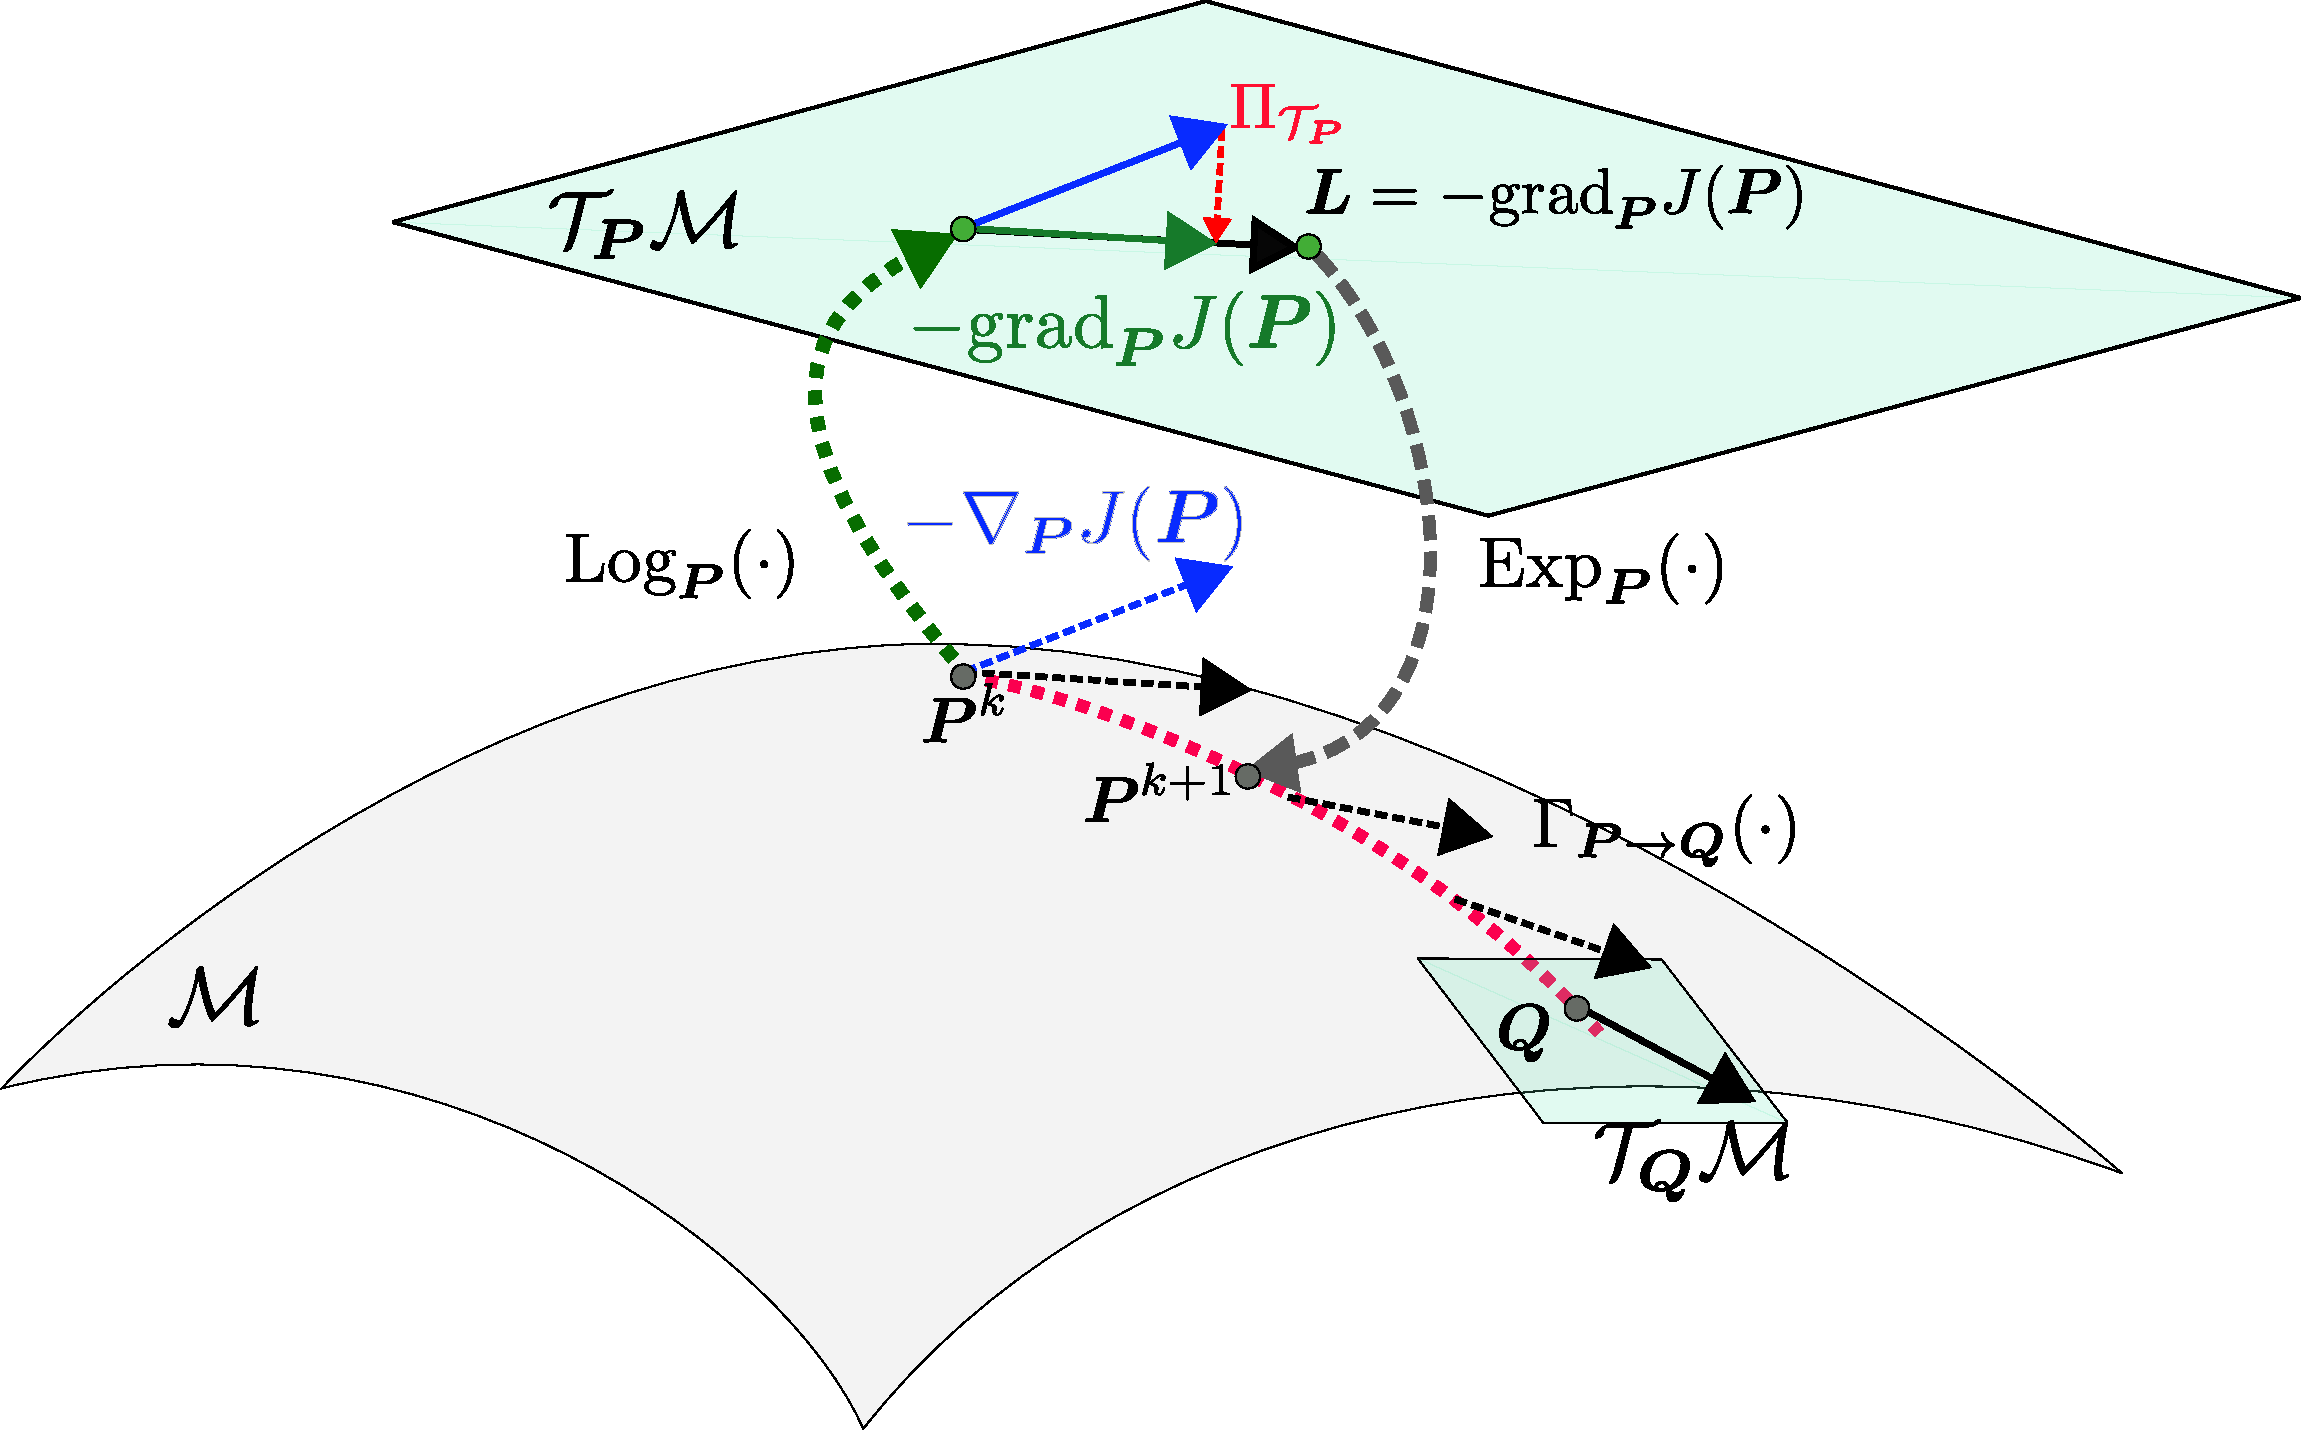
\includegraphics[width=0.5\textwidth]{manifold_operators.pdf}
	\hspace*{\fill}	
	\caption[] {\label{fig:manifold_operators}\textbf{Gradient descent on a manifold.} The figure illustrates the curved space of the manifold and its associated tangent space. The logarithmic and exponential maps enable to project a point from the tangent space to the manifold space and vice-versa.}
\end{figure*}
% ---
The gradient descent methods discussed above are thought to operate in Euclidean (flat) spaces. Some of the operators and quantities that describe the kinematics and dynamics of a robot are elements of curved manifold spaces and hence are more difficult to update following the update rules of Euclidean gradient descent methods. Considering again a cost function $J\left(\bm{P}\right)$, the \emph{Riemannian gradient} at a point $\bm{P}$ in a manifold space $\mathcal{M}$ is the orthogonal projection of the gradient in ambient Euclidean space
% ---
\begin{equation}
	\bm{G} = \nabla J(\cdot)=\frac{\partial J}{\partial \bm{P}}\in \mathbb{R}^{n \times n}
\end{equation}
% ---
onto the associated tangent space $\mathcal{T}_{\bm{P}}\mathcal{M}$ \cite{Boumal2014Optimizationestimationmanifolds.}; that is,
% ---
\begin{equation}
	\text{grad}_{\bm{P}}J(\bm{P}) = \Pi_{ \mathcal{T}_{\bm{P}}}\left(\nabla J(\bm{P})\right) \in \mathcal{T}_{\bm{P}}\mathcal{M},
\end{equation} 
% ---
with the projection operator defined as
% ---
\begin{equation}
	\Pi_{ \mathcal{T}_{\bm{P}}}(\bm{G})\triangleq\bm{P}\left(\frac{\bm{G}+\bm{G}^T}{2}\right)\bm{P},
\end{equation} 
% ---
for all the points in the manifold \cite{Brooks2019Riemannianbatchnormalization}. As described in \cite{Bonnabel2013Stochasticgradientdescent}, Riemannian gradient descent uses
% ---
\begin{equation}
	\bm{P}^{k+1}= \text{Exp}_{\bm{P}^k}\left(-\gamma \text{grad}_{\bm{P}^k}J(\bm{P}^k)\right),
\end{equation} 
% ---
with $ \gamma \in (0,1]$, to compute the update to the parameter $\bm{P}$ on $\mathcal{M}$. The exponential map $ \text{Exp}_{\bm{P}^k}\left(\cdot\right)$ of a Riemannian manifold at a point $\bm{P}^k$ projects a point on the tangent space to the manifold space; i.e., $ \text{Exp}_{\bm{P}^k}: \mathcal{T}_{\bm{P}^k}\mathcal{M}\rightarrow \mathcal{M}$. Conversely, the logarithmic map takes a point on the manifold and projects it onto the associated tangent space; that is, $ \text{Log}_{\bm{P}^k}: \mathcal{M}\rightarrow \mathcal{T}_{\bm{P}^k}\mathcal{M}$. Fig.~\ref{fig:manifold_operators} illustrates these maps and their involvement in Riemannian gradient descent. The particular definitions for the exponential and logarithmic maps depend on the considered Riemannian manifold $\mathcal{M}$.

%Motivated by the stability and convergence speed of  AMSGrad, this dissertation makes use of its manifold version, the Riemannian AMS gradient descent ---RAMSGrad for short \cite{Becigneul2018Riemannianadaptiveoptimization}. Core steps for RAMSGrad involve computing the moving averages for the gradient and its Riemannian norm, as well as the aggregation of the previous gradients by considering the curvature of the manifold. \redtext{This algorithm will be discussed in more detailed in the next chapter}. 

Inspired by the stability and convergence speed of AMSGrad, this thesis utilizes its Riemannian counterpart, referred to as RAMSGrad for short \cite{Becigneul2018Riemannianadaptiveoptimization}. Essential features of RAMSGrad encompass the computation of moving averages for the gradient and its Riemannian norm, as well as the amalgamation of previous gradients, taking into account the curvature of the manifold. A more detailed discussion of this algorithm will be provided in the upcoming chapter.

%Likewise, the Riemannian gradient of a function $J(\bm{P})$ at a point $\bm{P}=(\bm{P}_1,\ldots,\bm{P}_N)\in\mathcal{M}^N$ is expressed by $
%\text{grad}_{\bm{P}}J=\left(\text{grad}_{\bm{P}_i}J_1, \ldots, \text{grad}_{\bm{P}_N}J_N\right)$;  with $\bm{P}_i\in\mathcal{M}_i$, i.e. defined on a product manifold.
%%
%Here the term $\text{grad}_{\bm{P}_i}J_i$ represents the Riemannian gradient of the partial map $
%J_i:\bm{Q}\in \mathcal{M}_i \mapsto f\left(\bm{P}_1,\ldots,\bm{P}_{i-1},\bm{Q},\bm{P}_{i+1},\ldots,\bm{P}_N\right)$. 

% ===========================================================================================
%                                           |                                               |
% -------------------------------------- SECTION -------------------------------------------|
%                                           |                                               |
% ===========================================================================================
\section{Chapter summary}
%This chapter presented an overview of the different concepts that relate to the understanding of the physical structure of the robot. The physical self, and its relation to embodiment, body morphology, and body schema were discussed. Particular emphasis was given to the body schema as it functions as a model representation of the physical structure of the robot. Its most important features were discussed and connections to model-based robotics were established to present the definition of the robot body schema that is used in this dissertation. The bodily features needed to construct the robot body schema were outlined and methods to learn its kinematics and dynamics, that is the description of body size and inertial properties, were discussed. Special attention was dedicated to body shape, understood as the mechanical arrangement of the joints and links, that is, the body topology. This body aspect is essential to characterize the kinematic and dynamic features. Relevant concepts from the fields of information and graph theory were provided to illustrate how performing network topology inference on the sensorimotor signals of a robot can lead to the inference of the mechanical structural connectivity. Lastly, modern implementations of gradient descent were revisited as they are relevant in the implementation of online learning schemes to extract the features of the robot body schema.

This chapter offers an overview of various concepts related to comprehending the physical structure of the robot. It delves into the physical self and its connections to embodiment, body morphology, and body schema. Special focus is given to the body schema, serving as a model representation of the robot's physical structure. The chapter discusses its key features and establishes connections to model-based robotics, presenting the definition of the robot body schema utilized in this dissertation. Essential bodily features required for constructing the robot body schema are outlined, and methods for learning its kinematics and dynamics, encompassing the description of body size and inertial properties, are examined. Emphasis is placed on body shape, defined as the mechanical arrangement of joints and links, i.e., the body topology, crucial for characterizing kinematic and dynamic features. Concepts from information and graph theory are introduced to illustrate how performing network topology inference on the robot's sensorimotor signals can infer mechanical structural connectivity. Lastly, the chapter revisits modern implementations of gradient descent, particularly relevant in implementing online learning schemes to extract features of the robot body schema.

% ===========================================================================================
%                                           |                                               |
% -------------------------------------- SECTION -------------------------------------------|
%                                           |                                               |
% ===========================================================================================
%\section{Body modeling in congenitally blind individuals}
%(1) The article "Influence of the Body Schema on Multisensory Integration: Evidence from the Mirror Box Illusion" in Scientific Reports - Nature discusses the influence of the body schema on multisensory integration, which is a fundamental aspect of robotic model learning.
%
%(2) The paper "Neuroplasticity in the blind and sensory substitution for vision" on ResearchGate explores neuroplasticity in the blind, which is relevant to understanding how the body schema is developed and adapted in the absence of vision, a concept that can be applied to robotics.
%
%(3) The article "Does visual experience influence arm proprioception and its lateralization? Evidence from passive matching performance in congenitally-blind and sighted adults" in ScienceDirect provides insights into the relationship between visual experience and proprioception, which is foundational to the development of the body schema and has implications for robotics.
%
%(4) The study "Degraded vision affects mental representations of the body" published on Taylor \& Francis Online discusses the impact of degraded vision on mental representations of the body, including the shift from a pictorial representation of the body to a somatosensory one, which is relevant to understanding the body schema in the context of robotic model learning.
%
%While these sources do not directly address the application of body schema to model learning in robotics, they provide valuable insights into the development and influence of the body schema, which can be extrapolated to understand its potential relevance to model learning in robotics.
%
%Citations:
%[1] https://www.nature.com/articles/s41598-017-04797-0
%[2] https://www.researchgate.net/publication/262840022_Neuroplasticity_in_the_blind_and_sensory_substitution_for_vision
%[3] https://www.sciencedirect.com/science/article/abs/pii/S030439402300294X
%[4] https://www.tandfonline.com/doi/full/10.1080/13506285.2023.2186997
